\documentclass{article}


\usepackage{PRIMEarxiv}
\usepackage[numbers]{natbib}

\usepackage[utf8]{inputenc} % allow utf-8 input
\usepackage[T1]{fontenc}    % use 8-bit T1 fonts
\usepackage{hyperref}       % hyperlinks
\usepackage{url}            % simple URL typesetting
\usepackage{booktabs}       % professional-quality tables
\usepackage{amsfonts}       % blackboard math symbols
\usepackage{nicefrac}       % compact symbols for 1/2, etc.
\usepackage{microtype}      % microtypography
\usepackage{lipsum}
\usepackage{fancyhdr}       % header
\usepackage{graphicx}       % graphics
\graphicspath{{media/}}     % organize your images and other figures under media/ folder

%Header
\pagestyle{fancy}
\thispagestyle{empty}
\rhead{ \textit{ }} 

% Update your Headers here
%\fancyhead[LO]{Running Title for Header}
%\fancyhead[RE]{Firstauthor and Secondauthor} % Firstauthor et al. if more than 2 - must use \documentclass[twoside]{article}

% my packages
\usepackage{amsmath,bm}
\usepackage{enumerate,enumitem}
\usepackage{array}
\newcolumntype{L}[1]{>{\raggedright\let\newline\\\arraybackslash\hspace{0pt}}m{#1}}
\newcolumntype{C}[1]{>{\centering\let\newline\\\arraybackslash\hspace{0pt}}m{#1}}
\newcolumntype{R}[1]{>{\raggedleft\let\newline\\\arraybackslash\hspace{0pt}}m{#1}}
\usepackage{multirow,multicol}
\usepackage{tikz}
\usetikzlibrary{positioning, shapes, decorations.markings, decorations.pathreplacing, decorations.pathmorphing, arrows, calc, matrix}
\usepackage{caption}
\usepackage{subcaption}
\usepackage{float}

% Optional math commands from https://github.com/goodfeli/dlbook_notation.
%%%%% NEW MATH DEFINITIONS %%%%%

% \usepackage{amsmath,amsfonts,bm}
\usepackage{amsmath,amsfonts}

\usepackage{pifont}


\newcommand{\R}{\mathbb{R}}


\def\va{{\mathbf{a}}}
\def\vg{{\mathbf{g}}}

% Sets
\def\sR{\mathbb{R}}
\def\sC{\mathbb{C}}
\def\sZ{\mathbb{Z}}
\def\sN{\mathbb{N}}
\def\sQ{\mathbb{Q}}

\def\sS{\mathcal{S}}



% Vectors
\def\vzero{{\mathbf{0}}}
\def\vone{{\mathbf{1}}}
\def\vmu{{\mathbf{\mu}}}
\def\vtheta{{\mathbf{\theta}}}
\def\va{{\mathbf{a}}}
\def\vb{{\mathbf{b}}}
\def\vc{{\mathbf{c}}}
\def\vd{{\mathbf{d}}}
\def\ve{{\mathbf{e}}}
\def\vf{{\mathbf{f}}}
\def\vg{{\mathbf{g}}}
\def\vh{{\mathbf{h}}}
\def\vi{{\mathbf{i}}}
\def\vj{{\mathbf{j}}}
\def\vk{{\mathbf{k}}}
\def\vl{{\mathbf{l}}}
\def\vm{{\mathbf{m}}}
\def\vn{{\mathbf{n}}}
\def\vo{{\mathbf{o}}}
\def\vp{{\mathbf{p}}}
\def\vq{{\mathbf{q}}}
\def\vr{{\mathbf{r}}}
\def\vs{{\mathbf{s}}}
\def\vt{{\mathbf{t}}}
\def\vu{{\mathbf{u}}}
\def\vv{{\mathbf{v}}}
\def\vw{{\mathbf{w}}}
\def\vx{{\mathbf{x}}}
\def\vy{{\mathbf{y}}}
\def\vz{{\mathbf{z}}}
\def\vzeta{{\mathbf{\zeta}}}

% Matrix
\def\mA{{\mathbf{A}}}
\def\mB{{\mathbf{B}}}
\def\mC{{\mathbf{C}}}
\def\mD{{\mathbf{D}}}
\def\mE{{\mathbf{E}}}
\def\mF{{\mathbf{F}}}
\def\mG{{\mathbf{G}}}
\def\mH{{\mathbf{H}}}
\def\mI{{\mathbf{I}}}
\def\mJ{{\mathbf{J}}}
\def\mK{{\mathbf{K}}}
\def\mL{{\mathbf{L}}}
\def\mM{{\mathbf{M}}}
\def\mN{{\mathbf{N}}}
\def\mO{{\mathbf{O}}}
\def\mP{{\mathbf{P}}}
\def\mQ{{\mathbf{Q}}}
\def\mR{{\mathbf{R}}}
\def\mS{{\mathbf{S}}}
\def\mT{{\mathbf{T}}}
\def\mU{{\mathbf{U}}}
\def\mV{{\mathbf{V}}}
\def\mW{{\mathbf{W}}}
\def\mX{{\mathbf{X}}}
\def\mY{{\mathbf{Y}}}
\def\mZ{{\mathbf{Z}}}
\def\mBeta{{\mathbf{\beta}}}
\def\mPhi{{\mathbf{\Phi}}}
\def\mLambda{{\mathbf{\Lambda}}}
\def\mSigma{{\mathbf{\Sigma}}}


% Expectation
% \def\eE{\mathop{\mathbb{E}}\limits}
\def\eE{\mathbb{E}}

% Probability
\def\pP{\mathbb{P}}

% Tilde
\def\tf{\tilde{f}}
\def\tS{\tilde{S}}
\def\wtF{\widetilde{\mathcal{F}}}
\def\whR{\widehat{R}}
\def\tvx{\tilde{\mathbf{x}}}
\def\ty{\tilde{y}}


\def\defeq{\overset{\textup{def}}{=}}
% \def\defeq{\overset{.}{=}}
\def\defone{\overset{\text{\ding{172}}}{=}}
\def\deftwo{\overset{\text{\ding{173}}}{=}}
\def\leqone{\overset{\text{\ding{172}}}{\leq}}
\def\leqtwo{\overset{\text{\ding{173}}}{\leq}}
\def\leqthree{\overset{\text{\ding{174}}}{\leq}}
\def\leqfour{\overset{\text{\ding{175}}}{\leq}}
\def\eqone{\overset{\text{\ding{172}}}{=}}
\def\eqtwo{\overset{\text{\ding{173}}}{=}}
\def\eqthree{\overset{\text{\ding{174}}}{=}}
\def\eqfour{\overset{\text{\ding{175}}}{=}}
\def\geqfive{\overset{\text{\ding{176}}}{\geq}}
%\documentclass{MITstyle}

%\usepackage[table]{xcolor}
\usepackage{chngcntr}
\usepackage{hyperref}
\usepackage{microtype}

\title{A Lightweight and Extensible Cell Segmentation and Classification Model for Whole Slide Images}

\author{Nikita Shvetsov~$^{1, }$\footnote{Correspondence e-mail: nikita.shvetsov@uit.no}, Thomas K. Kilvaer~$^{2, 3}$, Masoud Tafavvoghi~$^{4}$, Anders Sildnes~$^{1}$, \\ Kajsa Møllersen~$^{4}$, Lill-Tove Rasmussen Busund~$^{5, 6}$, Lars Ailo Bongo~$^{1}$ \\
%
\vspace{1em} % Space between authors and afilliations
%
\normalfont{\small $^{1}$Department of Computer Science, UiT The Arctic University of Norway}\\
\normalfont{\small $^{2}$Department of Oncology, University Hospital of North Norway}\\
\normalfont{\small $^{3}$Department of Clinical Medicine, UiT The Arctic University of Norway}\\
\normalfont{\small $^{4}$Department of Community Medicine, UiT The Arctic University of Norway}\\
\normalfont{\small $^{5}$Department of Medical Biology, UiT The Arctic University of Norway} \\
\normalfont{\small $^{6}$Department of Clinical Pathology, University Hospital of North Norway} %\vspace{2em}
}

\begin{document}
\maketitle

\section*{Abstract}

% \begin{abstract}
% Developing clinically useful cell-level analysis tools in digital pathology remains challenging due to limitations in dataset granularity, inconsistent annotations, computational demands of advanced models, and difficulties in integrating new technologies into clinical workflows. To address these challenges, we propose a multi-faceted solution that enhances data quality, model performance, and usability to create a lightweight and extensible cell segmentation and classification model.

% First, we update data labels by employing a cross-relabeling process that refines the labels of two existing datasets, PanNuke and MoNuSAC, to create a new unified dataset with enhanced granularity, encompassing seven distinct cell types. Second, we leverage the H-Optimus foundation model as a fixed encoder to improve feature representation for simultaneous cell segmentation and classification tasks. Third, to address the computational demands of foundation models, we employ knowledge distillation to reduce model size and complexity while maintaining comparable performance. Finally, to facilitate integration into clinical workflows, we integrate the distilled model into the QuPath software, a widely used open-source platform in digital pathology.

% Our results demonstrate improvements in cell segmentation and classification performance using the H‑Optimus-based model compared to a CNN-based model. Specifically, the average $R^2$ improved from 0.575 to 0.871, and the average $PQ$ score improved from 0.450 to 0.492, indicating better alignment with actual cell counts and enhanced segmentation and classification quality. Furthermore, the distilled student model maintains performance comparable to the larger foundation model while reducing the parameter count by a factor of 48.
% Overall, by reducing computational complexity and integrating it into existing workflows, the proposed approach may significantly impact diagnostic processes, reduce the workload of pathologists, and contribute to improved patient outcomes. Though our approach shows potential enhancements in efficiency and usability of cell segmentation and classification models in digital pathology, extensive validation is needed to deploy these models in clinical practice.
% \end{abstract}

%%% shortened abstract
\begin{abstract}
Developing clinically useful cell-level analysis tools in digital pathology remains challenging due to limitations in dataset granularity, inconsistent annotations, high computational demands, and difficulties integrating new technologies into workflows. To address these issues, we propose a solution that enhances data quality, model performance, and usability by creating a lightweight, extensible cell segmentation and classification model. 

First, we update data labels through cross-relabeling to refine annotations of PanNuke and MoNuSAC, producing a unified dataset with seven distinct cell types. Second, we leverage the H-Optimus foundation model as a fixed encoder to improve feature representation for simultaneous segmentation and classification tasks. Third, to address foundation models' computational demands, we distill knowledge to reduce model size and complexity while maintaining comparable performance. Finally, we integrate the distilled model into QuPath, a widely used open-source digital pathology platform. 

Results demonstrate improved segmentation and classification performance using the H-Optimus-based model compared to a CNN-based model. Specifically, average $R^2$ improved from 0.575 to 0.871, and average $PQ$ score improved from 0.450 to 0.492, indicating better alignment with actual cell counts and enhanced segmentation quality. The distilled model maintains comparable performance while reducing parameter count by a factor of 48. By reducing computational complexity and integrating into workflows, this approach may significantly impact diagnostics, reduce pathologist workload, and improve outcomes. Although the method shows promise, extensive validation is necessary prior to clinical deployment.
\end{abstract}
\clearpage

\section{Introduction}
In digital pathology, accurate segmentation and classification of cells are crucial for many diagnostic, prognostic, and predictive analyses \cite{Jaber_Beziaeva_etal._2019,Lin_Pan_etal._2022,Park_Ock_etal._2022,Shen_Choi_etal._2024}. Nowadays, developments in computational pathology offer multiple solutions \cite{H._Qu_P._Wu_etal._2020,Javed_Mahmood_etal._2020} to utilize cell-level datasets to train machine learning models that solve these problems. The quality and specificity of training datasets are critical for robust and accurate models. Adhering to the principle of "garbage in, garbage out", it is essential to ensure that these datasets are extensively and accurately labeled with distinct classes that reflect the diverse biological characteristics of different cell types. Unfortunately, the number of open-source datasets comprising such high-quality annotations is limited. Existing cell segmentation datasets \cite{Gamper_Koohbanani_etal._2019,Graham_Vu_etal._2019,Verma_Kumar_etal._2021} may offer extensive annotations for certain cell types while providing more general labels for others. For example, in PanNuke, which is one of the largest open-source datasets comprising labeled cells, various types of morphologically and functionally different inflammatory cells like macrophages and lymphocytes are clustered in a broad "inflammatory" class. Consequently, these classes are frequently omitted from analyses or aggregated into broader meta-classes \cite{Gamper_Koohbanani_etal._2020} and likely interfere with other cell classes included in the dataset. This and similar inconsistencies in annotation granularity limit the ability of machine learning models to learn the comprehensive and nuanced features necessary for accurate cell segmentation and classification. To address these challenges, methods for refining and standardizing dataset annotations are essential to enhance the quality of training data.

A complementary approach to mitigate the absence of high-quality training data is the use of foundation models. Foundation models as encoders are defined as large-scale, versatile networks pre-trained on vast, diverse datasets using self-supervised learning, contrasting with convolutional neural network (CNN) pre-trained encoders that rely on supervised learning with labeled data. In practice, foundation models leverage enormous amounts of weakly or unlabeled data from millions of whole slide images (WSIs) and employ self-attention mechanisms to capture long-range dependencies and global context \cite{Chen_Ding_etal._2024,Saillard_Jenatton_etal._2024,Vorontsov_Bozkurt_etal._2024,Xu_Usuyama_etal._2024}. As a consequence, foundation models are able to produce transferable feature representations across different cell types and tissue environments. The feature representations can be leveraged by decoder networks to produce segmentation masks and pixel-level classifications. Because foundation models have comprehensive feature representations, they can be effectively fine-tuned using much smaller amounts of cell-level data compared to the large datasets needed to train models from scratch. Furthermore, foundation models incorporate adversarial training elements or contrastive learning \cite{Chen_Ding_etal._2024,Xu_Usuyama_etal._2024}, enhancing their resilience and adaptability by exposing them to challenging and varied scenarios during training. This may result in more generalizable models, often making them well-suited for diverse and complex tasks in digital pathology.

Despite the inherent advantages of foundation models, their deployment for practical use faces its own obstacles. In particular, they require substantial computational power, financial investments and rigorous testing to ensure reliability and efficacy for a given task \cite{Akkus_Dangott_etal._2022,Dragomir_Cocuz_etal._2022,Go_2022,Jafri_Farooqui_etal._2024}. Moreover, while foundation models enhance feature representation and performance, they depend on the quality of available annotations for decoder fine-tuning and, like any other model, cannot resolve existing inconsistencies or ambiguities in data labels. Therefore, there remains a critical need for solutions that address both data quality and practical deployment considerations.
Further, integrating new technologies into existing clinical workflows often encounters resistance, as it necessitates adjustments to established diagnostic processes. So, there is a need to develop solutions that could be integrated into current practices, minimizing the burden on medical professionals to adopt new tools \cite{King_Williams_etal._2023}.

Existing solutions \cite{Goldsborough_Philps_etal._2024,Hörst_Rempe_etal._2024}, while addressing some aspects of these challenges, fall short in providing a comprehensive approach. To address the data quality and clinical deployment issues, we propose a multi-faceted solution that encompasses data refinement, model optimization, and integration with existing pathology tools (\hyperref[fig:fig1]{Figure 1}). The outcome is a lightweight cell segmentation and classification model that can be integrated into digital pathology workflows for practical clinical use.

\begin{figure}[h!]
    \centering
    \includegraphics[width=\textwidth, height=0.82\textheight, keepaspectratio]{images/Figure_1.pdf}
    \caption{Overview of the proposed solution, including 1) Data refinement using cross-relabeling, 2) Teacher model development and fine tuning, 3) Student model optimization with knowledge distillation and 4) Student model and QuPath integration}
    \label{fig:fig1}
\end{figure}
\clearpage

Our approach begins with preparing the data for the fine-tuning and training of the machine learning models. We create a refined dataset, acquired via cross-relabeling two cell-level datasets, enhancing annotation specificity and consistency of the labeled data. Subsequently, we create a cell segmentation and classification model based on the foundation model. We leverage the foundation model as a fixed encoder and fine-tune a decoder using the refined dataset to improve generalization across diverse tissue- and cell types.
To ensure that the model remains lightweight and deployable in a possibly resource-constrained environment, we employ knowledge distillation to approximate the functionality of the foundation model. Finally, to facilitate the practical application of our model in digital pathology workflows, we integrate it with the QuPath \cite{Bankhead_Loughrey_etal._2017} application. Each methodological component contributes to the overarching goal of enhancing model performance, generalizability, and usability in clinical settings.

The primary contributions of this paper are:
\begin{enumerate}
    \item \textit{Data labels refinement through cross-relabeling:}
    
    We propose a new method for refining labels of cell-level datasets through cross-relabeling. This method employs classification models to re-label broad and ambiguous instances, resulting in a more diverse dataset. Our evaluation demonstrates that these classification models achieve high accuracy on test subsets, indicating the reliability of the method for label refinement.

    \item \textit{Enhanced model performance via foundation models:}
    
    We employ a foundation model as a feature extractor for the cell segmentation and classification task. In comparison with training a CNN model from scratch, the foundation model backbone only needs fine-tuning, which significantly reduces training time, computational resources and data requirements. We show that using a foundation model encoder leads to better performance in cell segmentation and classification networks than using a CNN-based encoder. This improvement may enable the model to generalize more effectively across various tissue types and imaging methods.
    
    \item \textit{Model optimization through knowledge distillation:}
    
    We show that a smaller student model trained using knowledge distillation on the refined dataset obtained via our cross-relabeling approach from a foundation model achieves comparable performance in cell segmentation and quantification tasks. As a result, this model is more suitable for deployment in environments without high-performance computing resources.
    
    \item \textit{Integration with QuPath:}
    
    We integrate the distilled cell segmentation and classification model into QuPath, a widely used open-source digital pathology platform, to accelerate clinical adaptation by enabling pathologists to more easily incorporate advanced computational tools into their existing workflows.
\end{enumerate}

Through these methodological steps, we aim to bridge the gap between advanced machine learning techniques and practical clinical applications, making accurate and efficient digital pathology accessible in a broader range of healthcare settings.

\section{Refining Existing Datasets Using Cross-Relabeling}
To address the limitations of sparse and ambiguous labeling of cell-level datasets, we propose a generalizable cross-relabeling strategy that can be applied to any dataset containing broadly categorized or imprecisely labeled cell types. This approach involves training and subsequently leveraging classification models to refine broad categories into more specific or biologically relevant classes.
When applied to cell-level data, the methodology includes extracting individual cell images from the dataset patches, preprocessing these images to standardize the size and accommodate partial cells, and then training deep learning classifiers capable of distinguishing between the finer cell subtypes within the coarser categories. 
To illustrate our approach, we focus on the PanNuke \cite{Gamper_Koohbanani_etal._2020, Gamper_Koohbanani_etal._2019} and MoNuSAC \cite{Verma_Kumar_etal._2021} datasets that we have used to train models for cell quantification in our previous works \cite{Shvetsov_Grønnesby_etal._2022,Shvetsov_Sildnes_etal._2024}. We find that for better cell differentiation we have to introduce more granular labels. PanNuke includes a broad classification of "inflammatory" cells, encompassing lymphocytes, macrophages, and neutrophils. Each cell type differs significantly in structure, function, and clinical relevance. Conversely, MoNuSAC uses the label "epithelial" for a class that comprises both benign epithelial cells and malignant neoplastic cells. This practice makes it challenging to differentiate between benign and malignant epithelial cells in the dataset, which is a critical distinction when identifying tumor areas within tissue samples. To address these issues, we implement a cross-relabeling strategy as shown in \hyperref[fig:fig2]{Figure 2}. The key components are two classification models: one is trained on singular cell images from PanNuke data to classify the epithelial meta-class into epithelial and neoplastic classes. The other is trained on MoNuSAC to refine the inflammatory class into lymphocytes, neutrophils, and macrophages.

\begin{figure}[h!]
    \centering
    \includegraphics[width=\textwidth]{images/Figure_2.pdf}
    \caption{Refined dataset generation via cross relabeling}
    \label{fig:fig2}
\end{figure}

The refining approach consists of three consecutive steps. The first is the preprocessing step, in which we extract individual cells from both datasets (\hyperref[fig:fig3]{Figure 3}). The specifics of PanNuke and MoNuSAC patch preparation before cell preprocessing are provided in \hyperref[chap:S1]{Appendix S1}.

\begin{figure}[h!]
    \centering
    \includegraphics[width=\textwidth]{images/Figure_3.pdf}
    \caption{Cell instances preprocessing including (1) cell map extraction, (2) bounding box delineation, (3) adjusting cell boxes and (4) cropping and resizing of cell images}
    \label{fig:fig3}
\end{figure}

During preprocessing, we extract cell type maps from the ground truth label mask and calculate bounding boxes around each cell instance. To accommodate partial cells at patch borders, a common issue in cropped patch images, we employ mirror padding and extend the field of view of the cell label by 15 pixels to capture adjacent cells. We then crop and resize the identified regions to $64 \times 64$ pixels using bicubic interpolation.

The preprocessed PanNuke dataset comprises 68,031 neoplastic and 23,207 epithelial cell images, while MoNuSAC comprises  33,104 lymphocytes, 1,252 neutrophils, and 1,695 macrophages, which we subsequently use in training cell classification models and classifying the cell image data \hyperref[fig:S2]{Appendix Figure S2 (1)}. 

The next step is to train two distinct ResNet50-based classifiers tailored to address the specific labeling challenges inherent in each dataset. We use ResNet50 for classification models due to its proven effectiveness for image classification tasks in histopathology \cite{pan2022reviewmachinelearningapproaches}, and its compatibility with small images. For the PanNuke dataset, we design the classifier, trained on MoNuSAC data, to disaggregate the heterogeneous "inflammatory" cell category into distinct subtypes: lymphocytes, macrophages, and neutrophils. Similarly, for the MoNuSAC dataset, the classifier is trained on PanNuke data and distinguishes between benign and malignant epithelial cells within the overarching "epithelial" label. By applying these targeted classifiers to their respective datasets, we assign more specific labels to individual cell instances, thus enabling us to create a unified dataset.
To ensure a balanced representation of classes, we train both models on datasets that had been equalized to match the size of the least represented class. Thus, we obtain datasets comprising 23,207 samples per class for PanNuke and 1,252 samples per class for MoNuSAC data. Next, we partition both of them into training (70\%), validation (20\%), and testing (10\%) subsets. To mitigate the risk of overfitting, we use a single dropout layer with a rate of p=0.5 in both models and data augmentation using randomized color perturbations, rotation, and horizontal and vertical flipping. We employ AdamW optimizer and the cross-entropy loss function for the training criterion.

To evaluate the two trained models, we measure the classification accuracy on the respective test subsets. The accuracies on the test subset for both classifiers are presented in \hyperref[tab:1]{Table 1}. The PanNuke model achieves an average accuracy of 93.57\%, with higher accuracy for neoplastic cells (96.06\%) compared to epithelial cells (86.26\%). The confusion matrix in Figure A3.1 shows that the model predominantly distinguishes accurately between epithelial and neoplastic tissues, with a substantial number of correct classifications and relatively few misclassifications. The MoNuSAC model demonstrates an average accuracy of 98.92\%, excelling in classifying lymphocytes (99.67\%) and macrophages (94.12\%), with lower performance for neutrophils (85.71\%). The confusion matrix in Figure A3.2 shows that the model identifies lymphocytes and performs reasonably well with macrophages and neutrophils.

\begin{table}[h!]
\renewcommand{\arraystretch}{1.5}
  \centering
  \caption{Cell classification results for PanNuke and MoNuSAC trained models (CI 95\%).}
  \label{tab:1}
  \begin{tabular}{|l|c|c|}
   \hline
   %\rowcolor{gray!30}
    Accuracy               & PanNuke model              & MoNuSAC model              \\
    \hline
    Average      & 0.936 (0.931--0.941)         & 0.989 (0.986--0.993)        \\
    \hline
    Neoplastic   & 0.961 (0.956--0.965)         & -                          \\
    \hline
    Epithelial   & 0.863 (0.849--0.877)         & -                          \\
    \hline
    Lymphocytes  & -                          & 0.997 (0.995--0.999)        \\
    \hline
    Neutrophils  & -                          & 0.857 (0.796--0.918)        \\
    \hline
    Macrophages  & -                          & 0.941 (0.906--0.976)        \\
    \hline
  \end{tabular}
\end{table}

Finally, during the last step, we use the model trained on PanNuke data for epithelial cells in MoNuSAC and the model trained on MoNuSAC for the inflammatory cells class in PanNuke. Specifically, we use classifier models to relabel epithelial cells in MoNuSAC and inflammatory cells in PanNuke data. Then we combine cells with refined labels and the rest of the cells in both datasets to create a refined dataset (\hyperref[fig:S2]{Appendix Figure S2 (2)}). The process of relabeling cells and visualizing them on a patch is shown in \hyperref[fig:fig4]{Figure 4}. The cell counts in the refined dataset are provided in \hyperref[tab:S4]{Appendix Table S4}.

\begin{figure}[h!]
    \centering
    \includegraphics[width=\textwidth, height=0.42\textheight, keepaspectratio]{images/Figure_4.pdf}
    \caption{Cell relabeling procedure for epithelial and inflammatory cell classes}
    \label{fig:fig4}
\end{figure}

%\hfill

Relabeling and combining datasets have been explored in a prior study \cite{Parulekar_Kanwat_etal._2023}, where consecutive fine-tuning on multiple datasets was employed to account for hierarchical class label structures. While the method presented in \cite{Parulekar_Kanwat_etal._2023} is intuitive, it often lacks consistency and requires multiple fine-tuning runs, which can be cumbersome and time-consuming. 
In contrast, cross-relabeling simplifies this process by using specialized classification models tailored to each dataset's specific labeling challenges. This approach provides better transparency and produces a unified dataset encompassing seven distinct cell types across multiple tissue samples, enhancing data diversity for further model training or fine-tuning.

Despite these improvements, cross-relabeling does not entirely resolve issues related to poor labeling quality or the amount of labeled data. Specifically, our results show lower accuracies persist for underrepresented classes, such as macrophages, which may stem from a limited sample availability and intrinsic challenges in distinguishing these cells based solely on H\&E staining. Furthermore, while our method enhances label specificity, it relies on the initial quality of the broad labels; thus, any fundamental inaccuracies in the original annotations can propagate through the relabeling process. Addressing the overall problem of limited data labels may require integrating additional data sources or utilizing complementary immunohistochemical staining methods.
Although the reported performance metrics are obtained from evaluations on the native test sets of each dataset, it is important to note that the primary application of these classifiers is to perform cross-relabeling, where a model trained on one dataset (e.g., PanNuke) is applied to another (e.g., MoNuSAC) and vice versa. We acknowledge that a more systematic evaluation of cross-dataset generalization is needed and could be performed in future work.

Overall, the refined dataset produced by our approach can enhance the supervised training or fine-tuning of cell segmentation and classification models, especially those that utilize pre-trained foundation models to improve feature extraction robustness. In addition, these models can detect nuanced classes that enable researchers to conduct more detailed analyses of biological processes in computational pathology.

\section{Foundation models for robust cell segmentation and classification}

Accurate cell segmentation and classification in digital pathology are hindered by limited labeled data and the fact that conventional CNNs are unable to capture global contextual information due to their local receptive field constraints \cite{Gheflati_Rivaz_2022,Yang_Marcus_etal.}. Traditional approaches in cell quantification have predominantly relied on CNN encoders, such as ResNet50, given their proven effectiveness in semantic segmentation tasks \cite{Deshmane_2023,Graham_Vu_etal._2019,Mukasheva_Koishiyeva_etal._2024,Stringer_Wang_etal._2021}. However, approaches that include fine-tuning of pretrained CNNs, data augmentation, and stain normalization to partially increase data variability and address staining differences often fail to achieve the necessary generalization and robustness across diverse tissue types and staining conditions \cite{G._Wang_W._Li_etal._2018,Gao_Bagci_etal._2018,Karim_El_Khoury_Martin_Fockedey_etal._2021}.

To overcome these challenges, we leverage an encoder-decoder network that uses a foundation model as the encoder and a CNN upsampling decoder (\hyperref[fig:fig5]{Figure 5}) for simultaneous cell segmentation and classification in 2D patches extracted from WSIs. Foundation models with transformer-based architectures are viable alternatives to CNN-based encoders \cite{Shamshad_Khan_etal._2023,Sourget_2023}. They enable the creation of more advanced architectures that can decode or transform learned features more effectively \cite{Chen_Duan_etal._2023,Cheng_Misra_etal._2022,Xie_Wang_etal._2021}.

\begin{figure}[h!]
    \centering
    \includegraphics[width=\textwidth]{images/Figure_5.pdf}
    \caption{UNETR-like model with foundational model as backbone}
    \label{fig:fig5}
\end{figure}

By utilizing a transformer-based encoder, we incorporate global contextual information into the feature extraction process, which is a key advantage of such architectures \cite{Chen_Lu_etal._2021}. This foundation model integration facilitates accurate pixel-wise segmentation and classification without the need for extensive encoder training, thereby potentially improving generalization across varied cellular structures and tissue types.
In our implementation, we employ a modified UNETR \cite{Hatamizadeh_Tang_etal._2021} architecture that combines a vision transformer (ViT) \cite{Dosovitskiy_Beyer_etal._2021} encoder with a CNN-based decoder. The encoder utilizes the pretrained H-Optimus foundation model, which contains 1.1 billion parameters and is trained on over 500,000 H\&E stained WSIs \cite{Saillard_Jenatton_etal._2024}. We extract outputs from four evenly spaced transformer blocks $Z_i$, where $i \in [1, 14, 26, 38]$, to serve as residual connections for the CNN decoder. We select these blocks based on our observation that features from non-adjacent levels of the encoder lead to better overall performance on the test subset.

The CNN decoder upsamples the feature representations, acquired from the transformer blocks, to generate an intermediate vector that is handled by two task-specific layers that generate cell segmentation and classification masks. The first task-specific layer is the ‘Cellpose head’,  which is used to delineate cell instances. The layer generates horizontal and vertical gradient maps to form vector fields that are refined through gradient tracking in a post-processing step using the Cellpose algorithm \cite{Stringer_Wang_etal._2021}, known for its efficacy in cell segmentation tasks and generalizability across multiple domains \cite{Pachitariu_Stringer_2022,Stringer_Pachitariu_2024}. The second task-specific layer is the "Cell type head", which assigns labels to individual pixels. In the post-processing step, we determine the output classification label of each segmented cell instance by majority voting over the labeled pixels that comprise the cell in the segmentation map.

To evaluate model performance and measure the impact of adding a foundation model as backbone, we compare it to a ResNet50-based model. ResNet50 is a widely used solution for encoders in segmentation architectures in the medical domain \cite{Deshmane_2023,Graham_Vu_etal._2019,Mukasheva_Koishiyeva_etal._2024,Stringer_Wang_etal._2021}. For the H-Optimus-based model, we utilize frozen weights for the encoder and only fine-tune the decoder to take advantage of the extensive pre-training of the foundation model. For the ResNet50-based model we start with ImageNet \cite{Deng_Dong_etal.} weights and train both encoder and decoder parts. Hyperparameters for the training step are set to be identical, where possible, for comparable evaluation. 
For this evaluation, we deliberately use the PanNuke dataset to provide a standardized and controlled comparison between the H‑Optimus and ResNet50-based models (\hyperref[fig:S2]{Appendix Figure S2 (3)}). Specifically, we use two of the default PanNuke dataset splits (66\%) for training and validation, and reserve the third split (33\%) for testing.

To address the challenge of cell class imbalance in the PanNuke dataset, which is a common characteristic in most cell-level H\&E patch datasets, both models’ training processes employ a weighted loss function comprising cross-entropy and focal loss \cite{Lin_Goyal_etal._2018}. The focal loss component is adjusted with coefficients derived from each cell class' instance frequency, emphasizing learning from underrepresented classes and enhancing the model's sensitivity to rare but significant cellular patterns. The cross-entropy loss is augmented with spectral decoupling regularization \cite{Pezeshki_Kaba_etal._2021,Pohjonen_Stürenberg_etal._2022} and spatially varying label smoothing \cite{Islam_Glocker_2021}, which potentially stabilizes training and improves generalization in case of complex tissue morphologies. For optimization, we employ the \textit{AdamW} \cite{Loshchilov_Hutter_2019} to counter unbalanced class scenarios, with cosine annealing learning rate scheduler.

We utilize the scikit-learn library \cite{Van_der_Walt_Schönberger_etal._2014} and HoVer-Net \cite{Graham_Vu_etal._2019} implementations of $R^2$ (the coefficient of determination) and $PQ$ (panoptic quality) to evaluate our experiments. Complete mathematical formulations and detailed explanations of these metrics are provided in \hyperref[chap:S5]{Appendix S5}. To compute confidence intervals, we use nonparametric bootstrapping, where after calculating the metric on the full sample, we generated 1000 bootstrap replicates by resampling with replacement and then determined the 95\% confidence intervals as the 2.5th and 97.5th percentiles of the resulting empirical distribution.

%\hfill

The model comparisons are summarized in \hyperref[tab:2]{Table 2}. The H‑Optimus-based model achieves higher $R^2$ across all cell classes compared to the ResNet50-based model, which means that its predictions are more closely aligned with the PanNuke cell counts, indicating a stronger correlation with the observed data. Notably, the improvement of $R^2_{dead}$ may be an indicator of better global contextual representations provided by the foundation model backbone. In terms of segmentation and classification quality combined, measured by the PQ score, the H‑Optimus-based model demonstrates notable improvements across most cell classes. Overall, the average $R^2$ improved from 0.575 to 0.871, while the average $PQ$ score improved from 0.450 to 0.492, demonstrating better performance of the H-Optimus-based model.

\begin{table}[h!]
\renewcommand{\arraystretch}{1.5}
  \centering
  \caption{Cell quantification metrics for baseline and proposed models (CI 95\%).}
  \label{tab:2}
  \begin{tabular}{|l|c|c|}
    \hline
    %\rowcolor{gray!30}
    Metric             & Resnet50-based            & H-optimus-based              \\
    \hline
    $R^2_{neoplastic}$    & 0.681 (0.576--0.769)       & \textbf{0.941 (0.917--0.960)} \\
    \hline
    $R^2_{inflammatory}$  & 0.863 (0.778--0.903)       & \textbf{0.949 (0.918--0.966)} \\
    \hline
    $R^2_{connective}$    & 0.600 (0.488--0.698)       & 0.609 (0.436--0.772)          \\
    \hline
    $R^2_{dead}$          & 0.097 (-11.389--0.669)     & 0.925 (0.404--0.982)          \\
    \hline
    $R^2_{epithelial}$    & 0.635 (0.490--0.747)       & \textbf{0.930 (0.886--0.964)} \\
    \hline
    $PQ_{neoplastic}$       & 0.517 (0.499--0.535)       & \textbf{0.589 (0.575--0.604)} \\
    \hline
    $PQ_{inflammatory}$     & 0.455 (0.429--0.482)       & \textbf{0.528 (0.507--0.549)} \\
    \hline
    $PQ_{connective}$       & 0.416 (0.400--0.431)       & \textbf{0.451 (0.436--0.465)} \\
    \hline
    $PQ_{dead}$             & 0.374 (0.342--0.408)       & 0.292 (0.209--0.365)          \\
    \hline
    $PQ_{epithelial}$       & 0.488 (0.460--0.519)       & \textbf{0.599 (0.579--0.618)} \\
    \hline
  \end{tabular}
\end{table}

Our results  show that integrating the H‑Optimus foundation model within the UNETR architecture enhances the model's ability to segment and classify cells across diverse tissues from PanNuke data. The pretrained transformer encoder provides robust feature representations, resulting in higher average $R^2$ and $PQ$ scores compared to the CNN-based model. This leads to more reliable cell quantification and more accurate downstream analysis. Additionally, the streamlined fine-tuning process reduces computational overhead and training time, making the model more adaptable for new data.

Despite these advancements, the foundation model-based approach does not fully resolve all challenges related to cell segmentation and classification. We observe lower metric scores for underrepresented classes in the training data. Furthermore, foundation models typically encompass billions of parameters, resulting in substantial computational and memory requirements. It therefore poses challenges for deployment in resource-constrained environments, limiting their practical applicability in certain clinical settings.

\section{Model optimization via Knowledge Distillation}

To address the limitations posed by the extensive size of foundation models, we implement knowledge distillation — a model compression technique that leverages the teacher-student paradigm \cite{Hinton_Vinyals_etal._2015}. By training a smaller, more efficient student model to replicate the output of a larger, pre-trained teacher model, we retain performance while significantly reducing the model's complexity and resource requirements (\hyperref[fig:fig6]{Figure 6}).

\begin{figure}[h!]
    \centering
    \includegraphics[width=\textwidth, height=0.45\textheight, keepaspectratio]{images/Figure_6.pdf}
    \caption{Knowledge distillation framework for training a student model using a pre-trained teacher}
    \label{fig:fig6}
\end{figure}

We employ knowledge distillation to compress the H‑Optimus-based teacher model into a more efficient student model. The teacher model is the modified UNETR architecture with the H‑Optimus foundation model described in the previous chapter. The student model is based on a UNet architecture augmented with residual connections and incorporates a smaller ViT encoder with 9 million parameters \cite{Steiner_Kolesnikov_etal._2022,Wightman_2019}. 

First, we fine-tune the teacher model using the refined dataset from the cross-relabeling procedure (Section 2). Initially we train the decoder of the teacher model while keeping the encoder weights frozen. We split the refined dataset into train (70\%), validation (20\%) and test (10\%) subsets (\hyperref[fig:S2]{Appendix Figure S2 (4)}). During fine-tuning, we use the train and validation subsets, while leaving the test subset for model evaluation. We set the training procedure and model hyperparameters to be identical to those that were used to demonstrate the utility of foundation models for the simultaneous cell segmentation and classification task.

Next, we perform knowledge distillation from teacher to student using the refined dataset used to fine-tune the teacher model. The student model is trained to replicate the teacher model's outputs. We utilize a specialized loss function that aligns the student's predicted probability distribution with the teacher's, incorporating the teacher's class probability distribution derived from the output. Following the methodology of Hinton et al. \cite{Hinton_Vinyals_etal._2015}, we experiment with various hyperparameter settings for the temperature ($T$) and the balancing coefficients ($\alpha$ and $\beta$) in the loss function. We vary $T$ from 1 to 20 and adjust $\alpha$ and $\beta$ to balance the distillation and student losses. Through iterative tuning and evaluation, we identify that setting $T=14$, $\alpha=0.3$, and $\beta=0.7$ yields a configuration that converges and closely approximates the teacher model's performance during training.

Finally, we assess the performance of both models using the $R^2$ and $PQ$ (defined in \hyperref[chap:S5]{Appendix S5}) on the test set of the refined dataset (\hyperref[tab:3]{Table 3}). We observe that the 95\% confidence intervals overlap for most cell types, so we cannot claim statistically significant performance differences between the teacher and student models. One exception appears in the neoplastic class. The teacher model produces an $R^2$ of 0.919, while the student model shows an $R^2$ of 0.852. In addition, the student model achieves higher $PQ$ values for the neoplastic and connective classes, though the confidence intervals show overlap.

\begin{table}[h!]
\renewcommand{\arraystretch}{1.5}
  \centering
  \caption{Cell quantification metrics for teacher and distilled student models (CI 95\%).}
  \label{tab:3}
  \begin{tabular}{|l|c|c|}
    \hline
    %\rowcolor{gray!30}
    Metric & Teacher & Student \\
    \hline
    $R^2_{neoplastic}$    & \textbf{0.919} (0.898--0.939) & 0.852 (0.800--0.891) \\
    \hline
    $R^2_{lymphocyte}$    & 0.969 (0.956--0.977)         & 0.969 (0.956--0.978) \\
    \hline
    $R^2_{connective}$    & 0.694 (0.548--0.809)         & 0.618 (0.469--0.741) \\
    \hline
    $R^2_{dead}$          & 0.755 (0.400--0.908)         & 0.424 (0.100--0.731) \\
    \hline
    $R^2_{epithelial}$    & 0.922 (0.870--0.958)         & 0.843 (0.738--0.917) \\
    \hline
    $R^2_{macrophage}$    & 0.384 (-0.369--0.724)        & 0.704 (0.352--0.859) \\
    \hline
    $R^2_{neutrofil}$     & 0.854 (0.578--0.929)         & 0.833 (0.502--0.925) \\
    \hline
    $PQ_{neoplastic}$       & 0.581 (0.569--0.593)         & 0.601 (0.588--0.613) \\
    \hline
    $PQ_{lymphocyte}$       & 0.536 (0.520--0.553)         & 0.563 (0.544--0.579) \\
    \hline
    $PQ_{connective}$       & 0.436 (0.421--0.451)         & 0.457 (0.441--0.474) \\
    \hline
    $PQ_{dead}$             & 0.272 (0.235--0.315)         & 0.279 (0.201--0.369) \\
    \hline
    $PQ_{epithelial}$       & 0.522 (0.500--0.545)         & 0.530 (0.506--0.555) \\
    \hline
    $PQ_{macrophage}$       & 0.524 (0.459--0.588)         & 0.474 (0.405--0.543) \\
    \hline
    $PQ_{neutrofil}$        & 0.541 (0.490--0.592)         & 0.565 (0.522--0.607) \\
    \hline
  \end{tabular}
\end{table}


We further decompose the $PQ$ metric into its $SQ$ and $DQ$ components (\hyperref[tab:S6]{Appendix Table S6}). Both models produce nearly identical $SQ$ values, which indicates that they predict instance boundaries with similar precision. Although the student model shows some improvement in $DQ$ scores for certain classes, the confidence intervals overlap and do not confirm a statistically significant difference.

We observe that the student and teacher models yield comparable detection performance despite the student model using a much smaller and simpler architecture. A model with fewer parameters reduces the risk of overfitting when training data are scarce relative to the model’s complexity \cite{Farias_Ludermir_etal._2022}. The knowledge distillation process also encourages the student model to focus on the most generalizable detection features learned from the teacher. These factors enable the student model to achieve similar detection performance across different cell types.

Additionally, considering the model sizes reported in \hyperref[tab:4]{Table 4}, the distilled model achieves a significant reduction compared to the teacher model, with a 48-fold decrease in parameter count and a 5.5-fold reduction in on-disk size. In inference mode, the teacher model requires 16 GB of VRAM for a batch size of 32, while the distilled model only needs 3 GB of VRAM for the same batch size. These reductions make the distilled model significantly more practical for fine-tuning and deployment in resource-constrained environments.

\begin{table}[h!]
\renewcommand{\arraystretch}{1.5}
  \centering
  \caption{Parameter counts and size of teacher and distilled model}
  \label{tab:4}
  \adjustbox{max width=\textwidth}{%
  \begin{tabular}{|l|c|c|c|}
    \hline
    %\rowcolor{gray!30}
    Metric & H-optimus-based (Teacher) & mobileViT-based (Student) & Magnitude of difference \\
    \hline
    Parameters count       & 1,158,917,906   & \textbf{24,093,393}   & \textbf{48x}  \\
    \hline
    Estimated Total Size (MB) & 87,912       & \textbf{15,935}    & \textbf{5.5x} \\
    \hline
  \end{tabular}%
}
\end{table}

%\hfill

With recent advancements in complex network architectures and the use of pretrained encoders to achieve state-of-the-art performance \cite{Baumann_Dislich_etal._2024,Hörst_Rempe_etal._2024} in cell segmentation and classification tasks, model size, computational complexity, and processing times have increased. This limits the scalability and accessibility of these models. As we demonstrate, this may be mitigated using knowledge distillation. Studies in the field of natural language processing have demonstrated the efficacy of knowledge distillation in retaining the capabilities of the teacher model while achieving significant reductions in size and complexity \cite{Huangpu_Gao_2024,Sun_Yu_etal.}. 

We demonstrate the feasibility of knowledge distillation in digital pathology, specifically for cell segmentation and classification tasks. Moreover, we achieve this performance while also significantly reducing the parameter count. In addressing the challenge of knowledge transfer, we found that distillation from a transformer-based model to a smaller transformer is more straightforward than attempting to map transformer features to CNN blocks. In our experiments, using a CNN-based network as a student results in worse cell quantification performance due to the structural constraints of CNN feature space dimensions. 

Although our primary approach relies on a transformer-based student model that performs well, it can be further optimized to incorporate advantages from CNN architectures. For example, employing alternative techniques such as using ViT adapters \cite{Chen_Duan_etal._2023} or $1 \times 1$ convolutions to adjust feature map sizes may be beneficial for harnessing CNN advantages like enhanced local feature extraction. Moreover, if additional performance improvements are desired, the process can be further enhanced by applying supplementary knowledge distillation techniques, such as self-distillation \cite{Zhang_Song_etal._2019} or online distillation \cite{Houyon_Cioppa_etal._2023}.

Despite these promising results, further validation on independent datasets is necessary to fully understand the model's limitations. Underrepresented classes may pose challenges when addressing complex cases. Pathologists need to validate these models to adopt them in clinical settings. While the distilled models are smaller and more deployable, a technological gap persists because pathologists traditionally rely on established methods for inspecting WSIs and diagnosing diseases. Addressing the complexities involved in deploying models for inference and supporting pathologists in adopting new tools is essential for integrating these models into clinical workflows.

\section{Model integration with QuPath}
Digital pathology tools with graphical user interfaces are essential for visualizing and analyzing WSIs. To make our student model useful in clinical pathology workflows, it needs to be integrated into a tool that enables inspecting regions, creating annotations, and providing quantitative analyses of biomarkers. Therefore, we integrate the trained student model from the previous chapter into the QuPath open‑source platform \cite{Bankhead_Loughrey_etal._2017}. QuPath provides the required annotation, visualization, and analysis tools to interpret complex histological data, including workflows for cell segmentation, classification, and quantification (\hyperref[fig:fig7]{Figure 7}). 

\begin{figure}[h!]
    \centering
    \includegraphics[width=\textwidth]{images/Figure_7.pdf}
    \caption{Visualization of model-generated cell quantification annotations (left) and the corresponding unannotated slide (right) in QuPath}
    \label{fig:fig7}
\end{figure}

To identify the regions in a WSI critical for prognosticating tumor development, such as specific tumor areas or border regions without overlapping healthy tissue, the pathologist uses QuPath to outline these regions. Then, the pathologist initiates a cell segmentation and classification script through the QuPath interface for the selected regions. The resulting annotations and quantified cell information are then directly overlaid onto the WSI in the QuPath interface. Additional design and implementation details are in \hyperref[chap:S7]{Appendix S7}. 

Two common approaches for integrating deep learning models into QuPath are Java‑based native QuPath extensions \cite{Goldsborough_Philps_etal._2024} and the execution of RESTful API requests to a model server coupled with handling the response via an extension, as demonstrated in the application of cell segmentation models applied to immunofluorescence images \cite{Sugawara_2023}. While the community is actively working on these integration strategies, there is currently no universal solution that fully addresses all integration and performance requirements.

Extensions may offer better integration with QuPath, allowing slightly improved performance and more widespread usage of the built-in QuPath models, but they lack the flexibility to customize models and modify their behavior. For example, the newest version of QuPath includes models such as StarDist \cite{Weigert_Schmidt} and InstanSeg \cite{Goldsborough_Philps_etal._2024} that can perform cell segmentation. Both models pose limitations when applied to simultaneous cell segmentation and classification. StarDist performs well only on convex, round shapes by design, whereas some neoplastic, inflammatory, and connective cells exhibit complex and non-convex shapes. InstanSeg provides only semantic segmentation without assigning classes to the segmented cells.

%\hfill

In contrast, our approach offers an alternative integration strategy. It utilizes the paquo library to directly interact with QuPath’s internal application programming interface from within Python. This enables data exchange and processing without the need for intermediate conversion steps and provides greater control over model customization, retraining, and the incorporation of custom processing steps.

The integration of our custom model with QuPath underscores its potential to significantly enhance the diagnostic process by reducing the time burden on pathologists and enabling them to focus on more complex interpretative tasks using familiar software. Leveraging a tool that is already well-established among pathologists increases the likelihood of its adoption into daily clinical workflows. The quantitative data generated through the automated workflow is critical for both clinical decision-making and research, facilitating more accurate biomarker analysis, enabling robust statistical evaluations, and supporting hypothesis generation and testing. Additionally, by streamlining cell segmentation and classification, the tool enhances the scalability and reproducibility of pathological assessments, ultimately contributing to improved diagnostic accuracy and patient outcomes.

\section{Conclusion and future work}

In this study, we address critical challenges in digital pathology and tackle the usability and deployment issues of the developed models in standard computing environments without the need for high-performance computing systems. Our multi-faceted approach encompasses data refinement through cross-relabeling, leveraging foundation models for robust cell segmentation and classification, optimizing model performance via knowledge distillation, and integrating the optimized model into the QuPath software for practical application. This approach is used to construct a capable, versatile, and adjustable model for cell segmentation and classification, with enhanced performance and usability.

\begin{sloppypar}
While our approach shows potential in the field of computational pathology, certain limitations persist. 
For example, our implementation currently exhibits lower performance in detecting macrophages. 
This serves as an instance of the broader challenge of accurately identifying complex cell types. In order to address this issue, extending our approach to incorporate additional data sources, exploring alternative modeling approaches, and integrating other imaging modalities such as immunohistochemical staining may help improve detection accuracy. Moreover, although the distilled model reduces computational demands, integrating advanced deep learning models into clinical practice requires addressing technological gaps and potential resistance to adopting new tools within established diagnostic processes.
\end{sloppypar}

Future work could focus on several key areas to refine the proposed approach and facilitate its adoption in clinical environments. Enhancing the cell-relabeling process with additional datasets \cite{Graham_Jahanifar_etal._2021} could improve the representation of underrepresented cell types and enhance overall model performance. Also, incorporating additional data sources, such as multi-modal imaging or complementary staining methods, may address limitations related to cell type differentiation and class imbalance. Exploring other foundation models \cite{Vorontsov_Bozkurt_etal._2024,Zimmermann_Vorontsov_etal._2024} or introducing additional modalities \cite{Ding_Wagner_etal._2024,Vaidya_Zhang_etal._2025} may provide alternative architectures better suited to specific tasks or offer improved efficiency. Implementing more complex knowledge distillation techniques \cite{Houyon_Cioppa_etal._2023,Zhang_Song_etal._2019} could further optimize the model's performance and adaptability. Additionally, deeper integration with QuPath or other digital pathology software could provide pathologists more control over cell quantification analysis directly within the QuPath interface, thereby increasing accessibility and usability. Such enhancements would not only refine model performance but also ensure greater adaptability and scalability within various clinical environments. Finally, extensive validation of the model by pathologists and benchmarking against independent datasets are essential steps toward establishing the model's reliability and fostering confidence in its clinical utility.

\section*{Acknowledgments} 
This work was funded in part by the Research Council of Norway grant no. 309439 SFI Visual Intelligence, and the North Norwegian Health Authority grant no. HNF1521-20.

\bibliographystyle{IEEEtran}
\begin{sloppypar}
\begin{thebibliography}{99}

\bibitem{chaplot2020neural} Chaplot, Devendra Singh, et al. "Neural topological slam for visual navigation." Proceedings of the IEEE/CVF conference on computer vision and pattern recognition. 2020.

\bibitem{maksymets2021thda} Maksymets, Oleksandr, et al. "Thda: Treasure hunt data augmentation for semantic navigation." Proceedings of the IEEE/CVF International Conference on Computer Vision. 2021.

\bibitem{mezghan2022memory} Mezghan, Lina, et al. "Memory-augmented reinforcement learning for image-goal navigation." 2022 IEEE/RSJ International Conference on Intelligent Robots and Systems (IROS). IEEE, 2022.

\bibitem{al2022zero} Al-Halah, Ziad, Santhosh Kumar Ramakrishnan, and Kristen Grauman. "Zero experience required: Plug \& play modular transfer learning for semantic visual navigation." Proceedings of the IEEE/CVF Conference on Computer Vision and Pattern Recognition. 2022.

\bibitem{ye2021auxiliary} Ye, Joel, et al. "Auxiliary tasks and exploration enable objectgoal navigation." Proceedings of the IEEE/CVF international conference on computer vision. 2021.

\bibitem{chaplot2020object} Chaplot, Devendra Singh, et al. "Object goal navigation using goal-oriented semantic exploration." Advances in Neural Information Processing Systems 33 (2020)

\bibitem{ramakrishnan2022poni} Ramakrishnan, Santhosh Kumar, et al. "Poni: Potential functions for objectgoal navigation with interaction-free learning." Proceedings of the IEEE/CVF Conference on Computer Vision and Pattern Recognition. 2022.

\bibitem{ramrakhya2022habitat} Ramrakhya, Ram, et al. "Habitat-web: Learning embodied object-search strategies from human demonstrations at scale." Proceedings of the IEEE/CVF Conference on Computer Vision and Pattern Recognition. 2022.

\bibitem{mousavian2019visual} Mousavian, Arsalan, et al. "Visual representations for semantic target driven navigation." 2019 International Conference on Robotics and Automation (ICRA). IEEE, 2019.

\bibitem{dhariwal2021diffusion} Dhariwal, Prafulla, and Alexander Nichol. "Diffusion models beat gans on image synthesis." Advances in neural information processing systems 34 (2021)

\bibitem{ho2022classifier} Ho, Jonathan, and Tim Salimans. "Classifier-free diffusion guidance." arXiv preprint arXiv:2207.12598 (2022).

\bibitem{nichol2021glide} Nichol, Alex, et al. "Glide: Towards photorealistic image generation and editing with text-guided diffusion models." arXiv preprint arXiv:2112.10741 (2021)

\bibitem{brooks2023instructpix2pix} Brooks, Tim, Aleksander Holynski, and Alexei A. Efros. "Instructpix2pix: Learning to follow image editing instructions." Proceedings of the IEEE/CVF Conference on Computer Vision and Pattern Recognition. 2023.

\bibitem{fu2023guiding} Fu, Tsu-Jui, et al. "Guiding instruction-based image editing via multimodal large language models." arXiv preprint arXiv:2309.17102 (2023).

\bibitem{geng2024instructdiffusion} Geng, Zigang, et al. "Instructdiffusion: A generalist modeling interface for vision tasks." Proceedings of the IEEE/CVF Conference on Computer Vision and Pattern Recognition. 2024.

\bibitem{zhou2024minedreamer} Zhou, Enshen, et al. "Minedreamer: Learning to follow instructions via chain-of-imagination for simulated-world control." arXiv preprint arXiv:2403.12037 (2024).

\bibitem{zhou2023esc} Zhou, Kaiwen, et al. "Esc: Exploration with soft commonsense constraints for zero-shot object navigation." International Conference on Machine Learning. PMLR, 2023.

\bibitem{yu2023l3mvn} Yu, Bangguo, Hamidreza Kasaei, and Ming Cao. "L3mvn: Leveraging large language models for visual target navigation." 2023 IEEE/RSJ International Conference on Intelligent Robots and Systems (IROS). IEEE, 2023.

\bibitem{gadre2023cows} Gadre, Samir Yitzhak, et al. "Cows on pasture: Baselines and benchmarks for language-driven zero-shot object navigation." Proceedings of the IEEE/CVF Conference on Computer Vision and Pattern Recognition. 2023.

\bibitem{shah2023navigation} Shah, Dhruv, et al. "Navigation with large language models: Semantic guesswork as a heuristic for planning." Conference on Robot Learning. PMLR, 2023.

\bibitem{cai2024bridging} Cai, Wenzhe, et al. "Bridging zero-shot object navigation and foundation models through pixel-guided navigation skill." 2024 IEEE International Conference on Robotics and Automation (ICRA). IEEE, 2024.

\bibitem{yu2023co} Yu, Bangguo, Hamidreza Kasaei, and Ming Cao. "Co-NavGPT: Multi-robot cooperative visual semantic navigation using large language models." arXiv preprint arXiv:2310.07937 (2023).

\bibitem{wu2024voronav} Wu, Pengying, et al. "Voronav: Voronoi-based zero-shot object navigation with large language model." arXiv preprint arXiv:2401.02695 (2024).

\bibitem{qin2023mp5} Qin, Yiran, et al. "Mp5: A multi-modal open-ended embodied system in minecraft via active perception." arXiv preprint arXiv:2312.07472 (2023).

\bibitem{du2024learning} Du, Yilun, et al. "Learning universal policies via text-guided video generation." Advances in Neural Information Processing Systems 36 (2024).

\bibitem{ajay2024compositional} Ajay, Anurag, et al. "Compositional foundation models for hierarchical planning." Advances in Neural Information Processing Systems 36 (2024).

\bibitem{liang2024skilldiffuser} Liang, Zhixuan, et al. "Skilldiffuser: Interpretable hierarchical planning via skill abstractions in diffusion-based task execution." Proceedings of the IEEE/CVF Conference on Computer Vision and Pattern Recognition. 2024.

\bibitem{heusel2017gans} Heusel, Martin, et al. "Gans trained by a two time-scale update rule converge to a local nash equilibrium." Advances in neural information processing systems 30 (2017).

\bibitem{zhang2018unreasonable} Zhang, Richard, et al. "The unreasonable effectiveness of deep features as a perceptual metric." Proceedings of the IEEE conference on computer vision and pattern recognition. 2018.

\bibitem{brown2020language} Brown, Tom B. "Language models are few-shot learners." arXiv preprint arXiv:2005.14165 (2020).

\bibitem{podell2023sdxl} Podell, Dustin, et al. "Sdxl: Improving latent diffusion models for high-resolution image synthesis." arXiv preprint arXiv:2307.01952 (2023).

\bibitem{brohan2022rt} Brohan, Anthony, et al. "Rt-1: Robotics transformer for real-world control at scale." arXiv preprint arXiv:2212.06817 (2022).

\bibitem{brohan2023rt} Brohan, Anthony, et al. "Rt-2: Vision-language-action models transfer web knowledge to robotic control." arXiv preprint arXiv:2307.15818 (2023).

\bibitem{li2024manipllm} Li, Xiaoqi, et al. "Manipllm: Embodied multimodal large language model for object-centric robotic manipulation." Proceedings of the IEEE/CVF Conference on Computer Vision and Pattern Recognition. 2024.

\bibitem{shah2023vint} Shah, Dhruv, et al. "ViNT: A foundation model for visual navigation." arXiv preprint arXiv:2306.14846 (2023).

\bibitem{liu2024visual} Liu, Haotian, et al. "Visual instruction tuning." Advances in neural information processing systems 36 (2024).

\bibitem{hu2021lora} Hu, Edward J., et al. "Lora: Low-rank adaptation of large language models." arXiv preprint arXiv:2106.09685 (2021).

\bibitem{qin2023supfusion} Qin, Yiran, et al. "SupFusion: Supervised LiDAR-camera fusion for 3D object detection." Proceedings of the IEEE/CVF International Conference on Computer Vision. 2023.

\bibitem{qin2024worldsimbench} Qin, Yiran, et al. "Worldsimbench: Towards video generation models as world simulators." arXiv preprint arXiv:2410.18072 (2024).

\bibitem{yu2025gamefactory} Yu, Jiwen, et al. "GameFactory: Creating New Games with Generative Interactive Videos." arXiv preprint arXiv:2501.08325 (2025).

\bibitem{zhou2024code} Zhou, Enshen, et al. "Code-as-Monitor: Constraint-aware Visual Programming for Reactive and Proactive Robotic Failure Detection." arXiv preprint arXiv:2412.04455 (2024).

\bibitem{zhang2024ad} Zhang, Zaibin, et al. "AD-H: Autonomous Driving with Hierarchical Agents." arXiv preprint arXiv:2406.03474 (2024).

\bibitem{wang2024toward} Wang, Chaoqun, et al. "Toward Accurate Camera-based 3D Object Detection via Cascade Depth Estimation and Calibration." arXiv preprint arXiv:2402.04883 (2024).

\bibitem{huang2024story3d} Huang, Yuzhou, et al. "Story3d-agent: Exploring 3d storytelling visualization with large language models." arXiv preprint arXiv:2408.11801 (2024).

\bibitem{savinov2018semi} Savinov, Nikolay, Alexey Dosovitskiy, and Vladlen Koltun. "Semi-parametric topological memory for navigation." arXiv preprint arXiv:1803.00653 (2018).

\bibitem{majumdar2022zson} Majumdar, Arjun, et al. "Zson: Zero-shot object-goal navigation using multimodal goal embeddings." Advances in Neural Information Processing Systems 35 (2022): 32340-32352.

\bibitem{yadav2023offline} Yadav, Karmesh, et al. "Offline visual representation learning for embodied navigation." Workshop on Reincarnating Reinforcement Learning at ICLR 2023. 2023.

\bibitem{yadav2023ovrl} Yadav, Karmesh, et al. "Ovrl-v2: A simple state-of-art baseline for imagenav and objectnav." arXiv preprint arXiv:2303.07798 (2023).

\bibitem{sun2024fgprompt} Sun, Xinyu, et al. "FGPrompt: fine-grained goal prompting for image-goal navigation." Advances in Neural Information Processing Systems 36 (2024).

\bibitem{zhu2017target} Zhu, Yuke, et al. "Target-driven visual navigation in indoor scenes using deep reinforcement learning." 2017 IEEE international conference on robotics and automation (ICRA). IEEE, 2017.

\bibitem{koh2024generating} Koh, Jing Yu, Daniel Fried, and Russ R. Salakhutdinov. "Generating images with multimodal language models." Advances in Neural Information Processing Systems 36 (2024).

\bibitem{krantz2022instance} Krantz, Jacob, et al. "Instance-specific image goal navigation: Training embodied agents to find object instances." arXiv preprint arXiv:2211.15876 (2022).

\bibitem{schulman2017proximal} Schulman, John, et al. "Proximal policy optimization algorithms." arXiv preprint arXiv:1707.06347 (2017).

\bibitem{anderson2018evaluation} Anderson, Peter, et al. "On evaluation of embodied navigation agents." arXiv preprint arXiv:1807.06757 (2018).

\bibitem{lin2024navcot} Lin, Bingqian, et al. "NavCoT: Boosting LLM-Based Vision-and-Language Navigation via Learning Disentangled Reasoning." arXiv preprint arXiv:2403.07376 (2024).

\bibitem{NavGPT} Zhou, Gengze, Yicong Hong, and Qi Wu. "Navgpt: Explicit reasoning in vision-and-language navigation with large language models." Proceedings of the AAAI Conference on Artificial Intelligence.

\bibitem{hahn2021no} Hahn, Meera, et al. "No rl, no simulation: Learning to navigate without navigating." Advances in Neural Information Processing Systems 34 (2021): 26661-26673.

\bibitem{li2025t2isafety} Li, Lijun, et al. "T2ISafety: Benchmark for Assessing Fairness, Toxicity, and Privacy in Image Generation." arXiv preprint arXiv:2501.12612 (2025).

\bibitem{an2024agfsync} An, Jingkun, et al. "AGFSync: Leveraging AI-Generated Feedback for Preference Optimization in Text-to-Image Generation." arXiv preprint arXiv:2403.13352 (2024).


\end{thebibliography}
\end{sloppypar}

\clearpage
\beginsupplement
\section*{Appendix}
\renewcommand{\thesubsection}{S\arabic{subsection}}

\subsection{\label{chap:S1}PanNuke and MoNuSAC preprocessing}
The PanNuke dataset comprises a set of 7,901 RGB patches, each with dimensions of $256 \times 256$ pixels, which we set as the standard patch size for our analysis. In contrast, the MoNuSAC dataset encompasses 294 images of heterogeneous dimensions. To standardize the MoNuSAC images with our experiments, we implement a standardization protocol. Specifically, for images exceeding the dimensions of $256 \times 256$ pixels, we segment them into equal-sized patches and apply mirror padding to the remaining portions to avoid information loss at the peripherals. Patches with dimensions less than $128 \times 128$ pixels are excluded from the dataset due to the insufficient resolution to capture relevant cellular details. For patches where either dimension falls between 128 and 256 pixels, we employ upsampling to achieve the standard patch size. As a result, we obtain a total of 2,823 RGB patches derived from the MoNuSAC dataset for subsequent analysis. For additional details on the MoNuSAC data preparation process, refer to the source code \cite{Shvetsov_2025a}.
\clearpage

\subsection{\label{chap:S2}Data usage for the methodology}

\counterwithin{figure}{subsection}
\renewcommand{\thefigure}{S\arabic{subsection}}

\begin{figure}[h!]
    \centering
    \includegraphics[width=\textwidth, height=0.85\textheight, keepaspectratio]{images/A2.pdf}
    \caption{Overview of the methodology for cross-labeling, dataset refinement, and model comparison. (1) Cross-relabeling - training and testing cell classification models, (2) Cross-relabeling - using cell classification models to create refined dataset, (3) Fine-tuning and training models for comparison, (4) Student knowledge distillation with refined dataset}
    \label{fig:S2}
\end{figure}
\clearpage

\subsection{\label{chap:S3}Confusion matrices for classification models}
\counterwithin{figure}{subsection}
\renewcommand{\thefigure}{S\arabic{subsection}.\arabic{figure}}

\begin{figure}[h!]
    \centering
    \includegraphics[width=\textwidth, height=0.4\textheight, keepaspectratio]{images/A3_1.pdf}
    \caption{Confusion matrix for PanNuke trained model}
    \label{fig:S3.1}
\end{figure}

\begin{figure}[h!]
    \centering
    \includegraphics[width=\textwidth, height=0.4\textheight, keepaspectratio]{images/A3_2.pdf}
    \caption{Confusion matrix for MoNuSAC trained model}
    \label{fig:S3.2}
\end{figure}

\clearpage

\subsection{\label{chap:S4}Datasets cell counts}

\counterwithin{table}{subsection}
\renewcommand{\thetable}{S\arabic{subsection}}

\begin{table}[h!]
\renewcommand{\arraystretch}{2.0}
\centering
\caption{\label{tab:S4}Cell counts for PanNuke, MoNuSAC and refined datasets. Numbers in parentheses indicate preprocessed cell counts for cell classifier models training and testing.}
%\adjustbox{max width=\textwidth}{%
\begin{tabular}{|l|c|c|c|}
\hline
%\rowcolor{gray!30}
Cell type & PanNuke & MoNuSAC & Refined \\
\hline
Neoplastic & 77,403 (68,031) & - & 105,451 \\
\hline
Epithelial & 26,572 (23,207) & - & 29,926 \\
\hline
Epithelial (benign and malignant) & - & 31,402 & - \\
\hline
Inflammatory & 32,276 & - & - \\
\hline
Lymphocytes & - & 37,045 (33,104) & 65,275 \\
\hline
Neutrophils & - & 1,355 (1,252) & 3,833 \\
\hline
Macrophage & - & 1,842 (1,695) & 3,410 \\
\hline
Dead & 2,908 & - & 2,908 \\
\hline
Connective & 50,585 & - & 50,585 \\
\hline
\end{tabular}
%
%}
\end{table}



\clearpage

\subsection{\label{chap:S5}Definition of validation metrics}
\counterwithin{equation}{subsection}
\renewcommand{\theequation}{\arabic{equation}}

\subsubsection{\label{chap:S5.1}R\textsuperscript{2}}
The coefficient of determination, denoted as $R^2$, is a statistical measure that represents the proportion of variance in the dependent variable that is predictable from the independent variables. In the context of cell quantification in pathology, $R^2$ is used to assess how well the predicted quantities of different cell types in a patch align with the actual quantities observed in the ground truth data, with higher values representing more accurate quantification. $R^2$ is defined as
\begin{equation*}
R^2 = 1 - \frac{\sum_{i=1}^n (y_i - \hat{y}_i)^2}{\sum_{i=1}^n (y_i - \bar{y})^2},
\end{equation*}
where $y_i$ represents the actual number of cells of a specific type in the $i$-th image, $\hat{y}_i$ represents the predicted number of cells of that type in the $i$-th image, $\bar{y}$ is the mean of the actual numbers across all images, and $n$ is the total number of images in the dataset.

The $R^2$ metric has a range of $(-\infty, 1]$. An $R^2$ of 1 indicates perfect prediction, where all predicted values exactly match the actual values. An $R^2$ of 0 suggests that the model explains none of the variability of the response data around its mean. If $R^2$ is negative, it indicates that the model performs worse than a model that simply predicts the mean of the actual values for all observations.

\subsubsection{\label{chap:S5.2}PQ}
Panoptic Quality ($PQ$) is a comprehensive metric used to evaluate the performance of segmentation models in tasks that require both instance segmentation and classification. $PQ$ provides a single score that encapsulates both the detection accuracy (i.e., how many objects were correctly identified) and the segmentation quality (i.e., how accurately the objects' boundaries were delineated). This metric is particularly useful in multiclass scenarios where each pixel is classified into distinct categories, such as different cell types in pathology images.

$PQ$ is calculated as the product of two terms: Detection Quality ($DQ$) and Segmentation Quality ($SQ$). It can be expressed as
\begin{equation*}
PQ = DQ \cdot SQ,
\end{equation*}
where
\begin{equation*}
DQ = \frac{TP}{TP + 0.5\, FP + 0.5\, FN},
\end{equation*}
\begin{equation*}
SQ = \frac{\sum_{(p, g) \in \mathcal{M}} IoU(p, g)}{TP}.
\end{equation*}
In these formulas, $TP$ denotes the number of correctly matched instances between ground truth and prediction, $FP$ denotes the predicted instances that have no corresponding ground truth, $FN$ denotes the ground truth instances that were not detected, $IoU(p, g)$ is the Intersection over Union for a pair of matched instances $p$ (prediction) and $g$ (ground truth), and $\mathcal{M}$ is the set of matched pairs.

The $PQ$ metric is calculated for each class and is averaged across classes to provide a global performance measure.

The $PQ$ score has a range of $[0, 1.0]$, where a higher score indicates better performance in both detecting and segmenting the instances correctly. A $PQ$ of 1 signifies perfect identification and segmentation of all instances, whereas a $PQ$ of 0 indicates that no instances were correctly identified and segmented.

\clearpage

\subsection{\label{chap:S6}Segmentation and Detection quality metrics for teacher and student models}

\begin{table}[h!]
\renewcommand{\arraystretch}{2.0}
\centering
\caption{Segmentation and detection quality for student and teacher models (CI 95\%)}
\label{tab:S6}
%\adjustbox{max width=\textwidth}{%
\begin{tabular}{|l|c|c|}
\hline
%\rowcolor{gray!30}
Metric & Teacher & Student \\
\hline
$SQ_{neoplastic}$ & 0.819 (0.815--0.823) & 0.824 (0.819--0.828) \\
\hline
$SQ_{lymphocyte}$ & 0.795 (0.788--0.802) & 0.790 (0.783--0.796) \\
\hline
$SQ_{connective}$ & 0.770 (0.762--0.776) & 0.780 (0.772--0.786) \\
\hline
$SQ_{dead}$ & 0.659 (0.623--0.688) & 0.657 (0.624--0.695) \\
\hline
$SQ_{epithelial}$ & 0.780 (0.770--0.790) & 0.788 (0.779--0.797) \\
\hline
$SQ_{macrophage}$ & 0.788 (0.760--0.810) & 0.757 (0.730--0.783) \\
\hline
$SQ_{neutrofil}$ & 0.782 (0.761--0.801) & 0.775 (0.759--0.792) \\
\hline
$DQ_{neoplastic}$ & 0.706 (0.692--0.719) & 0.727 (0.712--0.741) \\
\hline
$DQ_{lymphocyte}$ & 0.675 (0.656--0.698) & 0.713 (0.691--0.734) \\
\hline
$DQ_{connective}$ & 0.566 (0.546--0.584) & 0.583 (0.565--0.602) \\
\hline
$DQ_{dead}$ & 0.410 (0.361--0.465) & 0.435 (0.306--0.561) \\
\hline
$DQ_{epithelial}$ & 0.668 (0.639--0.694) & 0.673 (0.644--0.702) \\
\hline
$DQ_{macrophage}$ & 0.657 (0.583--0.727) & 0.615 (0.531--0.703) \\
\hline
$DQ_{neutrofil}$ & 0.691 (0.625--0.753) & 0.729 (0.679--0.778) \\
\hline
\end{tabular}
%
%}
\end{table}

\clearpage

\subsection{\label{chap:S7}QuPath integration method}
We adopt an integration strategy leveraging the paquo \cite{Bayer_AG} library, a Python package that enables direct interaction with QuPath’s internal API, thereby facilitating seamless data exchange without intermediate conversion steps. The data processing pipeline (\hyperref[fig:S7]{Appendix Figure S7}) begins with the acquisition of WSIs and their associated annotations from QuPath, which are represented as Shapely \cite{Gillies_Wel_etal._2024} polygons. Utilizing paquo, we directly read, create, and modify these annotations and detections within a QuPath project in the Python environment. Images are then cropped using these polygons and processed by cell segmentation and classification models employing standard vision processing toolkits such as OpenCV, pyvips, and PyTorch. Additionally, QuPath employs Groovy scripts to initiate a Python process that starts the entire pipeline from QuPath graphical interface: fetching polygons, extracting images from them, and running deep learning model inference on the cropped images. 
The results are returned to QuPath, leveraging paquo's Python bindings to manipulate QuPath data while minimizing the computational overhead typically associated with cross-environment communication.

\counterwithin{figure}{subsection}
\renewcommand{\thefigure}{S\arabic{subsection}}

\begin{figure}[h!]
    \centering
    \includegraphics[width=\textwidth]{images/A7.pdf}
    \caption{QuPath integration workflow using Python environment}
    \label{fig:S7}
\end{figure}

Compared to traditional workflows that involve exporting annotations as GeoJSON, classifying them in Python, and reimporting them into QuPath, our approach offers several advantages. We eliminate the need to switch between programming languages, providing a cohesive and streamlined development process entirely within QuPath software and removing the necessity to use other tools. Meanwhile, we avoid storing annotations as intermediate JSON files unless required for external use or archiving. By conducting the entire inference and post-processing workflow within the Python environment, we leverage the power and flexibility of Python libraries for image processing and machine learning. This approach also enables adjustments to any set of labels and models, thereby improving its applicability.

%\hfill

The distilled model and QuPath integration code are packaged into a Docker container, enabling streamlined execution with the Docker engine. Detailed integration code and deployment instructions can be found in the GitHub repository \cite{Shvetsov_2025b}.

Despite these benefits, we acknowledge that the paquo library is a proof‑of‑concept project in its early development stage and has not been tested across all versions of QuPath.

\clearpage

\subsection{\label{chap:S8}Data and code availability statement}
All datasets, models, and code used in this study are publicly available and can be obtained from the repositories listed below. 
The PanNuke \cite{Gamper_Koohbanani_etal._2019} and MoNuSAC \cite{Verma_Kumar_etal._2021} datasets are publicly accessible, and download information along with detailed descriptions can be found in their respective articles. Preprocessing scripts for PanNuke and MoNuSAC data, as well as individual cell extraction scripts, are available on GitHub \cite{Shvetsov_2025a}. The H-Optimus foundation model used in our experiments can be downloaded from the HuggingFace repository \cite{hoptimus2024}, and model information is available on GitHub \cite{Saillard_Jenatton_etal._2024}. In addition, the integration code for QuPath and the distilled model packaged in a Docker container are provided in the repository \cite{Shvetsov_2025b}, and paquo Python library is available from the authors GitHub repository \cite{Bayer_AG}.
\clearpage

\end{document}


  
%% Title
\title{Convex Is Back: \\ Solving Belief MDPs With Convexity-Informed Deep Reinforcement Learning}



\author{
  Daniel Koutas \\
  ERA group \\
  TU Munich \\
  Munich, Germany\\
  \texttt{daniel.koutas@tum.de} \\
  %% examples of more authors
  \And
  Daniel Hettegger \\
  AIR chair \\
  TU Munich \\
  Munich, Germany\\
  \texttt{daniel.hettegger@tum.de} \\
  \And
  Kostas G. Papakonstantinou \\
  College of Engineering \\
  Penn State University \\
  Pennsylvania, USA\\
  \texttt{kpapakon@psu.edu} \\
  \And
  Daniel Straub \\
  ERA group \\
  TU Munich \\
  Munich, Germany\\
  \texttt{straub@tum.de} \\
}


\begin{document}
\maketitle

\vspace{-1em}
\begin{abstract}
We present a novel method for Deep Reinforcement Learning (DRL), incorporating the convex property of the value function over the belief space in Partially Observable Markov Decision Processes (POMDPs). We introduce hard- and soft-enforced convexity as two different approaches, and compare their performance against standard DRL on two well-known POMDP environments, namely the Tiger and FieldVisionRockSample problems. Our findings show that including the convexity feature can substantially increase performance of the agents, as well as increase robustness over the hyperparameter space, especially when testing on out-of-distribution domains. The source code for this work can be found at \url{https://github.com/Dakout/Convex_DRL}.
\end{abstract}


\section{Introduction}
\label{sec:Introduction}
%

Markov Decision Processes (MDPs) have become the standard formalism for solving sequential decision making problems \citep{van2012rlmdp}. For applications in which perfect observability cannot be assumed, MDPs can be extended to model the probabilistic decision process as a Partially Observable MDP (POMDP), which provides an efficient framework for optimal decision making under uncertainty \citep{kochenderfer2015decision,kaelbling1998planning,shani2013survey,braziunas2003pomdp,walraven2019point,oliehoek2008optimal,cassandra1994acting}. 

Classical dynamic programming (DP) and reinforcement learning RL are the two established solution methods for MDP and POMDPs. RL approaches are used to overcome the curse of dimensionality of DP methods, and additionally do not require a model of the environment \citep{kochenderfer2015decision}. Neural network (NN) based deep RL (DRL) applied to MDPs has been particularly successful, even in high dimensional problem settings \citep[e.g.,][]{mnih2013playingatari,mnih2015human,silver2016mastering,silver2018general}. Solving POMDPs is a more difficult task, but one approach is to directly handle the noisy observation-action history (or a variant thereof) \citep{koutas2024investigation,hettegger,giacomo}. In cases, where no environment model is available, this is the only option. If one has an environment model, then beliefs, i.e., a probability distribution over all system states, can be computed. Using beliefs can be computationally beneficial \citep{giacomo,koutas2024investigation}; however, most current approaches do not use DRL with beliefs. In this work, we propose to extend belief-based DRL solutions for POMDPs, by taking into account the theoretical property that the optimal value function is convex over the belief space. We hypothesize that introducing this informative property in the training process enables faster learning, and leads to better performance in out-of-distribution (OOD) domains.

We propose two approaches for convexity-enforcement of the value function in the training process, namely soft-enforced and hard-enforced convexity. 
The performance of convexity-informed DRL is examined for both convexity approaches applied to the Dueling Q-Network \citep{wang2016dueling} value-based architecture. Two benchmarks are used for performance comparison, which are the classic \emph{Tiger} \citep{kaelbling1998planning} and \emph{FieldVisionRockSample} (FVRS) \citep{ross2007aemsfvrs} problems. We show that when trained with the convexity modification, the involved NNs have stronger generalization performance compared to the standard training schedule and, in some cases, better training performance.

\textbf{Related work} \newline
Learning convex functions has a rich history in machine learning. However, the techniques developed in literature deal with explicitly defined target functions, e.g., including Karush-Kuhn-Tucker conditions of quadratic programs as differentiable layers \cite{amos2017optnet}, 
log-likelihoods in conditional random fields \cite{zheng2015rnncrf}, or energy functions in structured prediction energy networks \cite{belanger2016spen}. These methods are not applicable to DRL, where the value function is implicitly defined through the Bellman equation, and are thus not similar to our contribution.  

Regarding hard-enforced convex NNs for MDP problems, the closest work to this paper is a combination of Amos et al. \citep{amos2017inputconvexnns} and Sivaprasad et al. \citep{sivaprasad2021curious}. Amos et al. \citep{amos2017inputconvexnns} introduce fully and partially input convex neural networks, where the architectures include required skip connections at every layer. The focus of their work lies more on performing inference on the final convex NN to find the optimal input values. Their reference to the application on DRL focuses merely on perfectly observable and continuous action problems. They represent the negative Q-function with an input convex NN, and subsequently select the optimal action as a convex optimization problem over the NN output. However, they do not consider partially observable environments, as is the focus of this work. Sivaprasad et al. \citep{sivaprasad2021curious} define conditions to achieve input-output convexity with fully connected NNs without the need for skip connections, and convolutional architectures; however, they do not consider DRL implementations. 

Regarding soft-enforcement of convexity in NNs for MDPs or POMDPs, we are not aware of any related work. 

%
%
%
%
%%%%%%%%%%%%%%%%%%%%%%%%%%%%%%%%%%%%%%%%%%%%%%%%%%%%
%%%%%%%%%%%%%%%%%%%%%%%%%%%%%%%%%%%%%%%%%%%%%%%%%%%%
%%%%%%%%%%%%%%%%%%%%%%%%%%%%%%%%%%%%%%%%%%%%%%%%%%%%
%
%
%
%
%
\section{Belief MDP}
\label{sec:Belief_MDP}
Markov Decision Processes (MDP) provide an efficient framework for finding optimal solutions in sequential decision making problems, where the environment $E$ is stochastic, the consequence of the agent's actions is probabilistic, and the state of the environment is known \citep{puterman2014markov}. Partially observable MDPs (POMDPs) provide a natural extension, where the true environment state is not perfectly known; instead the agent receives imperfect observations \citep{kochenderfer2015decision}. The POMDP can be formulated as an MDP by replacing the system states $s_t \in \sS$ with the corresponding belief $b(s_t) = p(s_t \mid o_{1:t},a_{1:t-1})$, where $o_t \in \sO$ and $a_t \in \sA$ denote the received observation and action performed by the agent, respectively. As new information is available to the agent, the new belief states can be obtained with Bayesian updating \citep{kochenderfer2015decision,andriotis2019managing}:
%
\begin{equation}
\begin{aligned}
\label{eq_belief_update}
    b(s_{t+1})&=p(s_{t+1} \mid o_{t+1},a_t,\vect{b}_t) \\ %b'(s'_i) 
    &= \frac{O\left(o_{t+1} \mid s_{t+1}, a_t \right)}{p(o_{t+1} \vert \vect{b}_t,a_t)}
    %& \propto O\left(o_{t+1} \mid s_{t+1}, a_t \right)
    \sum_{s_t \in \sS} T\left(s_{t+1} \mid s_t, a_t\right) b(s_t),
\end{aligned}
\end{equation}
%
where $O$ and $T$ represent the observation and state transition probabilities, respectively, $p(o_{t+1} \vert \vect{b}_t,a_t)$ is the normalizing constant, and the belief vector $\vect{b}_t$ of
length $\abs{\sS}$ represents the collection of beliefs
$b(s_t) ~\forall s \in \sS$ \citep{andriotis2019managing}. 

Based on the chosen action and the underlying true state of the environment, the agent receives a reward $r_t \in \sR$ determined by the reward function $r(s_t, a_t)$, and the expected reward in a certain belief state can be obtained by $r(\vect{b}_t, a_t) = \sum_{s_t \in S} r(s_t,a_t)b(s_t)$. The decision-making rule, mapping beliefs to actions, is called policy $\pi(\vect{b}_t)$ \footnote{We limit this work to deterministic policies, but an extension to stochastic policies is possible}. 
%
The total expected discounted reward, or \emph{value function}, $V^{\pi}(\vect{b}_t)$, starting from $\vect{b}$ at time $t$ until the horizon $h$ under the policy $\pi$ is defined as \citep{walraven2019point, andriotis2019managing}:
%
%
\begin{equation}
\begin{aligned}
    \label{eq_value_function}
    V^{\pi}(\vect{b}_t) &= \E_{s_k\sim T,a_k\sim\pi, o_k\sim O}\left[\sum_{k=t}^h \gamma^{k-t} r(\vect{b}_k, a_k) \right],
\end{aligned}
\end{equation}
%
where $\gamma<1$ defines a discount factor. 
Similarly to \Eqref{eq_value_function}, one can define an \emph{action-value} function, $Q^{\pi}(\vect{b}_t, a_t)$, which defines the value of taking action $a$ at belief $\vect{b}$ at time $t$ until the horizon $h$ under the policy $\pi$:
%
\begin{equation}
\begin{aligned}
    \label{eq_qvalue_function}
    Q^{\pi}(\vect{b}_t, a_t)
    & =  \E_{s_k\sim T,a_k\sim\pi, o_k\sim O}\left[\sum_{k=t}^h \gamma^{k-t} r(\vect{b}_k, a_k) ~\bigg|~ a_t\right].
\end{aligned}
\end{equation}
%
The relationship between Equations \ref{eq_value_function} and \ref{eq_qvalue_function} is $V^{\pi}(\vect{b}_t) = Q^{\pi}(\vect{b}_t, \pi(\vect{b}_t))$. Having the Q-values, the agent's policy can be easily extracted by:
%
\begin{equation}
    \label{eq_policy}
    \pi(\vect{b}_t) = \argmax_{a_t \in \sA} Q^{\pi}(\vect{b}_t,a_t).
\end{equation}
%
The goal of the agent is to find the policy which maximizes the expected sum of discounted rewards. This optimal policy $\pi^*$ maximizes the value and action-values at every time $t$:
%
\begin{equation}
    \label{eq_opt_value_function}
    V^{*}(\vect{b}_t) := \left. V^{\pi}(\vect{b}_t)\right|_{\pi=\pi^*} = \max_{\pi} V^{\pi}(\vect{b}_t)
\end{equation}
%
%
\begin{equation}
    \label{eq_opt_qvalue_function}
    Q^{*}(\vect{b}_t, a_t) := \left. Q^{\pi}(\vect{b}_t, a_t)\right|_{\pi=\pi^*} = \max_{\pi} Q^{\pi}(\vect{b}_t, a_t),
\end{equation}
%
where $Q^{*}$ satisfies the recursive Bellman optimality condition \citep{cassandra1994acting}:% \citep{braziunas2003pomdp}:
%
\begin{equation}
\begin{aligned}
    \label{eq_opt_qvalue_function_bellman}
    Q^{*}(\vect{b}_t, a_t)
    & =  r(\vect{b}_t, a_t) + \gamma \sum \limits_{\vect{b}_{t+1} \in \sB} p(\vect{b}_{t+1} \vert \vect{b}_t,a_t) \max \limits_{a_{t+1} \in \sA} Q^{*}(\vect{b}_{t+1}, a_{t+1}).
\end{aligned}
\end{equation}
%
%
The focus of this work revolves around an important property of the optimal POMDP value function, namely that it should be convex over the belief space \citep{kochenderfer2015decision}. The different methods of enforcing this property are discussed in \Secref{sec:Convexity} and the application of the approaches to the Dueling architecture is discussed in \Secref{subsec:Convexity_informed_DRL}.

%
%
%%%%%%%%%%%%%%%%%%%%%%%%%%%%%%%%%%%%%%%%%%%%%%%%%%%%
%%%%%%%%%%%%%%%%%%%%%%%%%%%%%%%%%%%%%%%%%%%%%%%%%%%%
%%%%%%%%%%%%%%%%%%%%%%%%%%%%%%%%%%%%%%%%%%%%%%%%%%%%
%
%
%
%
%
%
\section{Deep Reinforcement Learning}
\label{sec:DRL}
%
One can use the recursive formulation in \Eqref{eq_opt_qvalue_function_bellman} to find the function $Q^*$, from which the optimal policy can then be extracted. Dynamic programming variants, such as, e.g., value or policy iteration, perform the optimization by iterating over all possible combinations of (belief) states, actions and observations \citep{kochenderfer2015decision}. However, due to the super-exponential growth in the value function complexity \citep{hauskrecht2000value}, this approach is not feasible for larger state and action spaces. By contrast, Neural Networks as universal function approximators \citep{hanin2019universal} have proven to be effective even in large state and action spaces, which has motivated their use for approximating $V,~Q,$ or $\pi$, in what is known as Deep Reinforcement Learning (DRL) \citep[e.g.,][]{andriotis2019managing,vinyals2019grandmaster}. 

One of the most prominent architectures for DRL are Deep Q-Networks (DQNs) \citep{mnih2013playingatari}, where the recursive \Eqref{eq_opt_qvalue_function_bellman} is reformulated into the temporal difference (TD) mean-squared error (MSE) loss function:
%
\begin{equation}
    \label{eq:MSE_td}
    MSE_t = \frac{1}{n_t} \sum_{i=1}^{n_t} \left|y^{(i)}-\Tilde{y}^{(i)} \right|^2
\end{equation}
%
where $y^{(i)}$ denotes an output sample of the NN and $~\Tilde{}~$ always denotes the counterpart of the target NN, whose weights get updated periodically \citep{mnih2015human}:
%
\begin{align}
    \label{eq:Q_output_NN}
    y^{(i)} &= Q(\vect{b}_t^{(i)}, a_t^{(i)} \mid \theta) \\
    \label{eq:Q_output_NN_target}
    \tilde{y}^{(i)} &= r_t^{(i)} + \gamma \max \limits_{a_{t+1}^{(i)} \in \sA} \Tilde{Q}(\vect{b}_{t+1}^{(i)}, a_{t+1}^{(i)} \mid \Tilde{\theta}).
\end{align}
%
Note that the Q-values in Equations \ref{eq:Q_output_NN} and \ref{eq:Q_output_NN_target} are DRL approximations of the optimal Q-function in \Eqref{eq_opt_qvalue_function}, and the TD-MSE in \Eqref{eq:MSE_td} is a sample-based approximation of the Bellman condition in \Eqref{eq_opt_qvalue_function_bellman}. The assumption is that, given enough samples and training, the DRL approximation should converge to the optimal solution.

%
%%%%%%%%%%%%%%%%%%%%%%%%%%%%%%%%%%%%%%%%%%%%%%%%%%%%
%%%%%%%%%%%%%%%%%%%%%%%%%%%%%%%%%%%%%%%%%%%%%%%%%%%%
%%%%%%%%%%%%%%%%%%%%%%%%%%%%%%%%%%%%%%%%%%%%%%%%%%%%
%
%
%
%
%
%
\section{Convex Neural Networks}
\label{sec:Convexity}
%
%%%%%%%%%%%%%%%%%%%%%%%%%%%%%%%%%%%%%%%%%%%%%%%%%%%%%%%%%%%%%%
%
\subsection{Convexity conditions for multi-dimensional functions}
\label{subsec:types_of_convexity}
%
%In this section we revise the conditions for convexity for multi-dimensional functions.

%
A function $f : \mathbb{R}^n \longrightarrow \mathbb{R}$ is convex if its domain is a convex set and for all $\vu, \vv$ in its domain, and all $t \in [0, 1]$, we have \citep{ahmadi2016theory}:
\begin{equation}
\label{eq:point_based_convexity}
    f(t \vu + (1 - t ) \vv ) \leq t f(\vu) + (1 - t)f(\vv).
\end{equation}
%
If $f$ is differentiable, one can define an alternative condition of convexity, which is equivalent to \Eqref{eq:point_based_convexity} \citep{ahmadi2016theory}:
%
\begin{equation}
    \label{eq:gradient_based_convexity}
    f(\vu)+\nabla_\vu f(\vu)^T(\vv-\vu) \leq f(\vv), \text { for all } \vu, \vv \in \operatorname{dom}(f).
\end{equation}
%
If $f$ is twice differentiable, then one can define yet another condition of convexity which is equivalent to Equations \ref{eq:point_based_convexity} and \ref{eq:gradient_based_convexity} %\Eqref{eq:point_based_convexity,eq:gradient_based_convexity}
\citep{ahmadi2016theory}:
%
\begin{equation}
    \label{eq:hessian_based_convexity}
    0 \preceq \mH (f)(\vu) = \nabla^2_\vu f(\vu) , \text { for all } \vu \in \operatorname{dom}(f),
\end{equation}
%
i.e., the Hessian matrix $\mH ( f) (\vu)$ must be positive semi-definite.
\Eqref{eq:point_based_convexity} defines convexity in terms of the function value at different points, whereas Equations \ref{eq:gradient_based_convexity} and \ref{eq:hessian_based_convexity}
%\Eqref{eq:gradient_based_convexity,eq:hessian_based_convexity}
define convexity via the first and second derivatives.

%
%%%%%%%%%%%%%%%%%%%%%%%%%%%%%%%%%%%%%%%%%%%%%%%%%%%%%%%%%%%%%%
%
\subsection{Hard-enforced convexity}
\label{subsec:hard-enforced_convexity}
%
The first obvious choice to satisfy convexity in the value function is to use an NN architecture which guarantees convexity. Considering a multi-layer perceptron of $k$ layers, where $h_i^{(l)}$ denotes the $i-$th neuron output in the $l-$th layer, then for an input $\vx\in \mathbb{R}^d$, $h_i^{(l)}$ is defined as \citep{sivaprasad2021curious}:
%
\begin{equation}
\label{eq:hidden_layer_output}
    h_i^{(l)}=\phi\left(\sum_j W_{i,j}^{(l)} h_j^{l-1}+b_i^{(l)}\right),
\end{equation}
%
with weights $W_{i,j}^{(l)}$, bias  $b_i^{(l)}$ and activation function $\phi(x)$. Further, $h_j^{(0)}=x_j(j=1, \ldots, d)$ and $h_j^{(k+1)}=y_j$ ($j^{\text {th }}$ NN output). Only two conditions are needed to ensure convexity of the final output y with
respect to the input x, namely \citep{amos2017inputconvexnns,sivaprasad2021curious}:
%
\begin{enumerate}[label=\roman*), ref=\roman*]
\item \label{item:nonnegative_weights} $0 \leq W_{i,j}^{(2: k+1)}$,
\item \label{item:phi_convex_and_nonnegative} $\phi$ \text{ is convex and a non-decreasing function.}
\end{enumerate}
%

Condition \ref{item:phi_convex_and_nonnegative}) can be achieved by using, e.g., Leaky Rectified Linear Unit (LReLU) \citep{maas2013rectifierlrelu}, Parametric ReLU (PReLU) \citep{he2015delvingprelu} or Exponential LU (ELU) \citep{clevert2015fastelu} activation functions. 

Condition \ref{item:nonnegative_weights}) needs to be enforced during the training process, e.g., by clipping negative weights to zero, taking absolute of weights, exponentiation of negative weights, or shifting negative weights after each iteration \citep{sivaprasad2021curious}. As this enforcement from outside interferes with the weight updates, and hence potentially hinders training, we also investigate the approach of soft-enforced convexity. Note that other, more complex approaches exist to enforce convexity, e.g., by representing weights as separate NN layers with absolute activation functions \citep{rashid2020monotonicqmix}. However, this would change the underlying architecture and complicate comparability between the approaches, which is why other enforcement options are left for future research. 


%
%%%%%%%%%%%%%%%%%%%%%%%%%%%%%%%%%%%%%%%%%%%%%%%%%%%%%%%%%%%%%%
%
\subsection{Soft-enforced convexity}
\label{subsec:soft-enforced_convexity}
%
Soft-enforced convexity mimics the idea of soft-enforced differential equations in Physics-Informed Neural Networks (PINNs) \citep{raissi2019pinn}. The core idea is to add a second term to the temporal loss function in \Eqref{eq:MSE_td}, which penalizes deviations of the target function from one of the convexity criteria outlined in \Secref{subsec:types_of_convexity}. Suppose we use the MSE loss function also for the second term, then the total MSE loss function is:
%
\begin{equation}
    \label{eq:mse_total_loss}
    MSE = MSE_t + c \cdot MSE_c,
\end{equation}
%
where the constant $c$ defines the relative weight of the TD- and convexity loss terms.

%
%
%%%%%%%%%%%%%%%%%%%%%%%%%%%%%%%%%%%%%%%%%%%%%%%
%%%%%%%%%%%%%%%%%%%%%%%%%%%%%%%%%%%%%%%%%%%%%%%
%
%
\section{Methodology}
\label{sec:Methodology}


\subsection{Convexity-informed DRL}
\label{subsec:Convexity_informed_DRL}
The NN architecture used throughout this work is the Dueling architecture \citep{wang2016dueling} depicted in \Figref{fig:dueling_architecture}.

\begin{figure}[H]
    \centering
    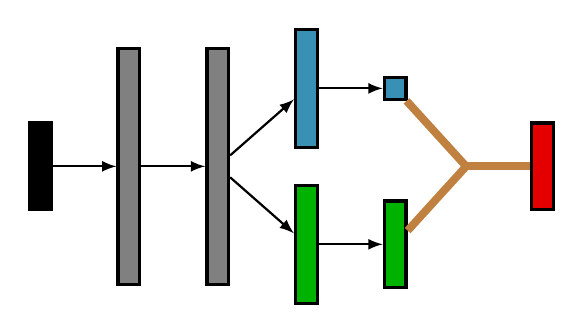
\begin{tikzpicture}
    \def\layerdist{0.81}
    \def\belheight{1.1}
    \def\belwidth{0.25*\belheight}
    \def\fcheight{3}
    
    \def\lettersep{0.2}
    \def\bndline{very thick}
    \def\arrthick{thick}
    \def\mergethick{0.1}
    
    \def\widthfac{1.39}
    %% nodes 
    % 0 node
    \coordinate (b) at (0,0);
    % first belief layer
    \node[rectangle, draw, fill=black, \bndline, minimum width = \belwidth cm, minimum height = \belheight cm, align=center, %label=above: $\vect{b}$
    ] (bel) at (b) {};
    % first fc layers
    \node[rectangle, draw, \bndline, minimum width = \belwidth cm, minimum height = \fcheight cm, right=\layerdist cm of bel, align=center, fill=gray] (fc1) {}; 
    \node[rectangle, draw, \bndline, minimum width = \belwidth cm, minimum height = \fcheight cm, right=\layerdist cm of fc1, align=center, fill=gray] (fc2) {};
    % arrows
    \draw[-latex, \arrthick] (bel) -- (fc1);
    \draw[-latex, \arrthick] (fc1) -- (fc2);
    % advantage & value fc
    \node[rectangle, draw, fill=black!30!cyan, \bndline, minimum width = \belwidth cm, minimum height = 0.5*\fcheight cm, right=\layerdist cm of fc2, yshift=0.33*\fcheight cm, align=center] (fcv) {}; 
    \node[rectangle, draw, fill=black!30!green, \bndline, minimum width = \belwidth cm, minimum height = 0.5*\fcheight cm, right=\layerdist cm of fc2, yshift=-0.33*\fcheight cm, align=center] (fca) {};
    % advantage & value
    \node[rectangle, draw, fill=black!30!cyan, \bndline, minimum width = 0.25*\belheight cm, minimum height = 0.25*\belheight cm, right=\layerdist cm of fcv, align=center, 
    %label=north: $V$
    ] (val) {};
    \node[rectangle, draw, fill=black!30!green, \bndline, minimum width = 0.25*\belheight cm, minimum height = \belheight cm,
    right=\layerdist cm of fca, align=center, 
    %label=south: $A$
    ] (adv) {};
    % arrows
    \draw[-latex, \arrthick] (fc2) -- (fcv);
    \draw[-latex, \arrthick] (fc2) -- (fca);
    \draw[-latex, \arrthick] (fca) -- (adv);
    \draw[-latex, \arrthick] (fcv) -- (val);
    % q-values
    \coordinate[right=3.7*\layerdist cm of fc2] (m);
    \node[rectangle, draw, fill=black!10!red, \bndline, minimum width = 0.25*\belheight cm, minimum height = \belheight cm, right=\layerdist cm of m, align=center,
    %label=north: $Q$
    ] (qval) {};
    % arrows
    \draw[line width=\mergethick cm, brown] (adv) -- (m);
    \draw[line width=\mergethick cm, brown] (val) -- (m);
    \draw[line width=\mergethick cm, brown] (m) -- (qval);
    \end{tikzpicture}
    %\captionsetup{width=\textwidth}
    \caption{Dueling network architecture, with the belief input (black), dense layers (gray), value stream (cyan), advantage stream (green) and Q-value output (red). Arrows indicate dense weights and the brown lines indicate computation without weights; adapted from \citep{wang2016dueling}.}
    \label{fig:dueling_architecture}
\end{figure}
%
\textbf{Hard-enforcement} of the value-convexity with respect to the belief input is performed by adjusting the weights according to condition i) in \Secref{subsec:hard-enforced_convexity} in the shared layers (gray), as well as the value stream (cyan) in \Figref{fig:dueling_architecture}. Condition ii) in \Secref{subsec:hard-enforced_convexity} is met by an appropriate choice of the activation function, which is kept identical for all layers.

\textbf{Soft-enforcement} of the value-convexity is performed by adding a second loss term according to \Eqref{eq:mse_total_loss}. Depending on the choice of the convexity criterion, namely 
point-based (p) in \Eqref{eq:point_based_convexity}, or gradient-based (g) in \Eqref{eq:gradient_based_convexity}, $MSE_c$ takes the form of:
%
\begin{equation}
    \label{eq:MSE_point_convexity}
    MSE_c^p = \frac{1}{n_c} \sum_{i=1}^{n_c} \max\left\{0,
    f(t^{(i)} \vu^{(i)} + (1 - t^{(i)}) \vv^{(i)} ) - t^{(i)} f(\vu^{(i)}) - (1 - t^{(i)})f(\vv^{(i)})\right\}^2
\end{equation}
%
%
\begin{equation}
    \label{eq:MSE_grad_convexity}
    MSE_c^g = \frac{1}{n_c} \sum_{i=1}^{n_c} \max\left\{0,
    f(\vu^{(i)})+\nabla_\vu f(\vu^{(i)})^T(\vu^{(i)}-\vv^{(i)}) - f(\vv^{(i)})\right\}^2.
    %f\left(b_{c,1}^i, b_{c,1}^{i}\right)^2
\end{equation}
%
The hessian-based condition in \Eqref{eq:hessian_based_convexity} cannot be translated into a loss function in a straightforward manner. A matrix $\mM$ is positive semi-definite (psd) if
%
\begin{equation}
    \label{eq:mat_pos_semi_def}
    \vx^T \mM \vx \geq 0 \quad \forall \vx \in \mathbb{R}^n.
\end{equation}
%
For 1D inputs, this is not a problem and the condition reduces to $\frac{d^2}{du^2}f(u)\geq0$ and the convex loss takes the form of
%
\begin{equation}
    \label{eq:MSE_hess_convexity_1D}
    MSE_c^{h,1D} = \frac{1}{n_c} \sum_{i=1}^{n_c} \max\left\{0,
    -\frac{d^2}{{du^{(i)}}^{2}} f(u_i)\right\}^2.
    %f\left(b_{c,1}^i, b_{c,1}^{i}\right)^2
\end{equation}
%
By contrast, for multidimensional inputs, \Eqref{eq:mat_pos_semi_def} can be checked in a sample based manner:
%
\begin{equation}
    \label{eq:MSE_hess_convexity_nD}
    MSE_c^{h,nD} = \frac{1}{n_c} \sum_{i=1}^{n_c} \frac{1}{n_{psd}} \sum_{j=1}^{n_{psd}} \max\left\{0,
    -{\vx^{(j)}}^T\mH ( f)(\vu^{(i)})\vx^{(j)}\right\}^2.
\end{equation}
%

$\vu^{(i)}$ and $\vv^{(i)}$ in Equations \ref{eq:MSE_point_convexity}, \ref{eq:MSE_grad_convexity}, \ref{eq:MSE_hess_convexity_1D} and \ref{eq:MSE_hess_convexity_nD} denote points $i=1,...,n_c$ sampled from the belief space, for which the respective convexity condition is checked; $\vx^{(j)}, ~j=1,...,n_{psd}$ denote points sampled from $\mathbb{R}^n$ for which the psd condition in \Eqref{eq:mat_pos_semi_def} checked.   

Once the respective soft enforcement method is chosen, belief points $\vect{b}^{(i)}$ (corresponding to $\vu^{(i)}$) are sampled from the problem-specific belief space and, together with other inputs, propagated through the network to obtain their values $V(\vect{b}^{(i)})$ (corresponding to $f(\vu^{(i)})$). In this work, we employ the Dueling architecture, hence the values can be obtained by propagation through the shared layers (gray) and subsequently through the value stream (cyan) of the network in \Figref{fig:dueling_architecture}.


\subsection{Numerical investigations}
\label{subsec:Hypotheses}
%
With numerical experiments, we test if enforcing convexity in the value function can improve the performance of DRL. Specifically, we test the following two hypotheses:

\emph{H1}: Enforcing convexity enables the DRL agent to learn faster due to restriction of the search space.

\emph{H2}: Convexity-informed DRL performs better in out-of-distribution domains due to improved extrapolation of the value function.

The two hypotheses are tested with experiments on two classic problems, namely the \emph{Tiger} \citep{kaelbling1998planning} and the \emph{FieldVisionRockSample} (FVRS) \citep{ross2007aemsfvrs} environments. Detailed descriptions of these problems are given in Sections \ref{sec:app_tiger_problem} and \ref{sec:app_fvrs_problem}. 

To test \emph{H1}, we train the DRL agent with and without enforcing convexity for a fixed number of training steps. We then compare the performance of the individual agents. 

To test \emph{H2}, we evaluate the performance of the agents for belief points which are not included in the training distribution. We achieve this by testing on observation functions which differ from the one used to train the agent. 
For the Tiger problem, we simply change the constant Tiger observation accuracy. For FVRS, the observation accuracy $p_{obs}$ for a rock depends on its Euclidian distance $d$ to the agent. The default (def) observation function is given as $p_{obs}^{def}(d) = 0.5+2^{-1-d/d_0}$, where the constant $d_0=(n-1)\sqrt{2}/4$ is chosen depending on the grid size $n$. To evaluate the agent on OOD data, we define the heaviside (heavi) function $p_{obs}^{heavi}(d) = 1$ for $d \leq d_0$ else $0.5$, where $d_0=1$. Furthermore, we also define a set of constant (const) observation functions  $p_{obs}^{const}(d) = c$, which do not depend on the distance between rock and agent. We use $c \in \{0.5, 0.6, ..., 1.0\}$. 

To allow for a fair comparison between the DRL with and without enforcing convexity we fix the hyperparameter optimization procedure beforehand. This prevents bias inflicted during the optimization (e.g., amount of time invested, number of samples, amount of steps). The detailed procedure used is reported in \Secref{sec:app_training_specifications}. After the hyperparameter search is conducted, we perform two separate investigations. Firstly, we evaluate the performance of each method over all hyperparameter samples, yielding a rough estimate of the robustness/sensitivity of each method with respect to changing hyperparameters. This approach is not customary in Machine Learning, which is why the corresponding results are only reported in Section \ref{sec:app_robustness_over_hyperparameters}. Secondly, we take the best hyperparameters of each search, and evaluate them over a certain number of runs. The results of this conventional approach are reported in the main text in Section \ref{sec:Results}.



The final policy of each agent is evaluated with a Monte Carlo (MC) approximation of the expected sum of discounted rewards $\hat{\rs}_r$. To evaluate the performance of each method, we employ boxplots, comprising the median, interquartile range, and maximum performance, which allows a more complete interpretation of the obtained results.  


%
%%%%%%%%%%%%%%%%%%%%%%%%%%%%%%%%%%%%%%%%%%%%%%%%%%%%
%%%%%%%%%%%%%%%%%%%%%%%%%%%%%%%%%%%%%%%%%%%%%%%%%%%%
%%%%%%%%%%%%%%%%%%%%%%%%%%%%%%%%%%%%%%%%%%%%%%%%%%%%
%
%
%
%
\section{Results}
\label{sec:Results}
%
% 

%
%
%
%
%%%%%%%%%%%%%%%%%%%%%%%%%%%%%%%%%%%%%%%%%%%%%%%%%%%%
%%%%%%%%%%%%%%%%%%%%%%%%%%%%%%%%%%%%%%%%%%%%%%%%%%%%
%%%%%%%%%%%%%%%%%%%%%%%%%%%%%%%%%%%%%%%%%%%%%%%%%%%%
%
%
%
%
%
%

%
\subsection{Computation time}
\label{subsec:computation_time}
%
All computations were performed on an Nvidia Tesla V100 GPU with 16GB RAM. For the Tiger problem, training for 5,000 steps and evaluating the policy with $2 \cdot 10^5$ MC samples took around 5 minutes. For FVRS, training for 50,000 steps and evaluating the policy with $10^4$ MC samples took approximately 60 minutes.


%
%%%%%%%%%%%%%%%%%%%%%%%%%%%%%%%%%%%%%%%%%%%%%%%%%%%%%%5
%%%%%%%%%%%%%%%%%%%%%%%%%%%%%%%%%%%%%%%%%%%%%%%%%%%%%%
%
\subsection{Tiger}
\label{subsec:Tiger}
%
%
We test the Tiger problem for all versions of enforced convexity (hard, point, grad and hess) as well as for the standard approach without enforced convexity. 

A visualization of the convexity violation of the standard DRL approach, as well as the corresponding value function correction of our proposed methods is shown in Section \ref{subsec:app_Tiger}.

We perform a hyperparameter search for  all convexity methods for various observation accuracies $p_{obs}=\{0.6, 0.8, 0.9, 1.0\}$. 
The evaluation of our hypotheses over the whole hyperparameter search is outlined in Section \ref{subsec:app_Tiger}. 

The test of $H1$ for the best hyperparameters yields no difference between the standard DRL approach and our proposed methods. This is due to the simplicity of the problem, where the majority of agents finds the optimal policy in the given amount of steps; thus, the mean performance over multiple seeds is close to the optimal performance with only little variation. 

%
\begin{figure}[H]
    \centering
    \includegraphics[width=0.85\textwidth]{figs/tiger_crossval_box_with_max.png}
    \caption{Boxplots (color-coded) over all optimal agents of a hyperparameter search with 200 runs for each convexity method. An optimal agent is one which has reached the optimal policy in the given amount of training steps, and the number of optimal agents was for grad: 178, hard: 68, hess: 69, None: 193, point: 183. The agents have been trained on $p_{obs}=1.0$ and cross-evaluated on $p_{obs}=\{0.5, 0.6, 0.7, 0.8, 0.9, 1.0\}$ with $10^5$ MC samples. Each boxplot includes the median as a blue horizontal line, interquartile range (IQR) as an opaque colored box, as well as the $1.5\cdot$IQR distances from the respective quartiles as whiskers; the maximum achieved value is marked with a colored hollow circle, other outliers are not visualized to avoid cluttering.
    }
    \label{fig:tiger_best_agents_cross_rewards}
\end{figure}
%

To test $H2$ for the best hyperparameters, we train the agents on a specific observation accuracy and cross-evaluate their performance on different observation accuracies. Since again, the majority of the hyperparameters converge to the optimal solution, we perform the cross-evaluation over all optimal agents. We observe that for agents trained on $p_{obs}=\{0.6, 0.8, 0.9\}$ there was no noticeable difference in the cross-evaluation performance between the individual convexity methods. Our explanation for this is that the optimal policy is characterized by two transition points from the action \emph{'listen'} to \emph{'open-left'/'open-right'}. Since these transition points lie very close to each other for $p_{obs} \in (0.5, 1.0)$ the methods do not have to perform a large extrapolation, which leads to almost identical results. For $p_{obs}=1.0$, however, the agent receives only the belief points $b=0.5$ and $b=1.0$ during training; thus, the agent does not know the location of the policy transition. For this case, the results are shown in Figure \ref{fig:tiger_best_agents_cross_rewards}, where the performance on the originally trained observation accuracy is the same for all agents (cf. $H1$), but the performance on $\{0.6, 0.8, 0.9\}$, in a distributional sense, is noticeably worse for the plain DRL approach compared to all convexity-enforced methods. This is reflected by lower medians (blue lines) and/or worse interquartile ranges. This shows that a well-behaved extrapolation of the value function can lead to better performance in out-of-distribution domains. We note that the max over all optimal agents is still the same for all methods. We suspect that this is again due to the simplicity of the Tiger problem.


%
%%%%%%%%%%%%%%%%%%%%%%%%%%%%%%%%%%%%%%%%%%%%%%%%%%%%%%5
%%%%%%%%%%%%%%%%%%%%%%%%%%%%%%%%%%%%%%%%%%%%%%%%%%%%%%
%
\subsection{FVRS}
\label{subsec:FVRS}
%
%

For FVRS, we do not consider the hard-enforced approach, because the value function is convex with regard to the belief inputs but not with regard to the position inputs. However, enforcing convexity of the neural network for only a subset of the inputs is not straightforward, hence we choose to leave this for further research. Moreover, we also do not consider the hessian approach to soft-enforced convexity. Computing second derivatives is simply too time-intensive for larger problems and one would choose other optimization algorithms (e.g., Newton) over gradient descent if second derivatives were available. 

Furthermore, for FVRS we use the LReLU activation functions, as we noticed that during training when the method converges to a stable policy (e.g., always go left), the weights of the hidden layers become high and negative. This ensures that the output is always -1 after passing through multiple ELU layers which yields the same Q-value for every possible combination of inputs. As a result, the method is stuck in this local minimum. To avoid this saturation, we switch to LReLU activation functions for the FVRS problem.

Moreover, we do hyperparameter searches for all convexity methods for the default (def) and heaviside (heavi) observation functions. We report the performances on the originally trained environment as well as the cross-evaluations on other observation functions in the same figures. The results over all samples are reported in Section \ref{subsec:app_FVRS}, whereas the performances of the hyperparameters over 10 runs for are shown in Figures \ref{fig:fvrs_def_cross_rewards_seed_eval} and \ref{fig:fvrs_heavi_cross_rewards_seed_eval}, respectively. When trained on the default setting (Figure \ref{fig:fvrs_def_cross_rewards_seed_eval}), both convexity approaches perform better than standard DRL, both on the original and all OOD domains. On the other hand, when trained on the heaviside observation function, the gradient-based approach emerges as the single clear winner over all observation functions. 

%
%
%
%%%%%%%%%%%%%%%%%%%%%%%%%%%%%%%%%%%%%%%%%%%%%%%%%%%%
%%%%%%%%%%%%%%%%%%%%%%%%%%%%%%%%%%%%%%%%%%%%%%%%%%%%
%%%%%%%%%%%%%%%%%%%%%%%%%%%%%%%%%%%%%%%%%%%%%%%%%%%%
%
%
%
%
%
%
\section{Conclusion and future work}
\label{sec:Conclusion}
%
In this work, we propose to extend DRL by enforcing the belief-convexity of the value function in the training process.
%To the best of our knowledge it is the first work towards a more theory-driven DRL approach.
We have shown that convexity-enforced DRL can yield notable improvements compared to the standard approach, such as better robustness over the hyperparameter space, as well as better mean performance of the best hyperparameters. Our approach performs particularly well when trained on edge case problems ($p_{obs}=1.0$ for Tiger and $p_{obs}=$ heavi for FVRS) and applying the policy to the standard problem formulation counterpart. This suggests that a well-behaved extrapolation of the value function leads to better policies when encountering OOD-data.

Based on the results in this work, we recommend the usage of the gradient-based enforcement, as it was better or at least equally good compared to the standard and point-based approach in every investigated setting.  

Several new empirical results are presented in this paper, yet there are still numerous open questions to be addressed. In particular, the largest performance gains of the convexity-enforced methods have been observed when training on edge cases, and extrapolating to the standard settings. This strongly suggests that these methods can improve performance when large extrapolations are needed. Hence, we anticipate particularly promising future research directions to be for cases where value extrapolations are required, i.e., in low data regimes, and higher dimensional problems. On the other hand, sampling-based techniques, as our soft-enforced methods, can face scalability challenges. Further investigations of the application to high-dimensional belief spaces are needed to fully grasp the potential of our proposed approaches.


Other potential research directions could be the investigation of convexity-informed DRL using actor-critic architectures, where the target directly is the value function, or the application of these methods to continuous-state POMDPs. Further developments of the convexity injection, e.g., heuristics for choosing an optimal value for $c$ in \Eqref{eq:mse_total_loss}, dynamic $c$ adjustments along the lines of LR-schedules, or including convexity loss every $k$ training steps to speed up the training process, can potentially lead to further improvements and training stability. 

%
\begin{figure}[H]
    \centering
    \includegraphics[width=0.85\textwidth]{figs/fvrs_def_seed_eval_1std.png}
    \caption{Best agents (color-coded) evaluated for 10 runs for each convexity method. The agents have been trained on the \textbf{default} observation function and are cross-evaluated on the heaviside (heavi) and a set of $p_{obs}=\{0.5, 0.6, 0.7, 0.8, 0.9, 1.0\}$ constant observation functions with $10^4$ MC samples. The figure shows the respective reward means (solid horizontal line) as well as $\pm$ 1 standard deviation (transparent bars).}
    \label{fig:fvrs_def_cross_rewards_seed_eval}
\end{figure}
%


%
\begin{figure}[H]
    \centering
    \includegraphics[width=0.85\textwidth]{figs/fvrs_heavi_seed_eval_1std.png}
    \caption{Best agents (color-coded) evaluated for 10 runs for each convexity method. The agents have been trained on the \textbf{heaviside} observation function and are cross-evaluated on the default (def) and a set of $p_{obs}=\{0.5, 0.6, 0.7, 0.8, 0.9, 1.0\}$ constant observation functions with $10^4$ MC samples. The figure shows the respective reward means (solid horizontal line) as well as $\pm$ 1 standard deviation (transparent bars).}
    \label{fig:fvrs_heavi_cross_rewards_seed_eval}
\end{figure}
%



%
%
%
%
%
%%%%%%%%%%%%%%%%%%%%%%%%%%%%%%%%%%%%%%%%%%%%%%%%%%%%
%%%%%%%%%%%%%%%%%%%%%%%%%%%%%%%%%%%%%%%%%%%%%%%%%%%%
%%%%%%%%%%%%%%%%%%%%%%%%%%%%%%%%%%%%%%%%%%%%%%%%%%%%
%
%
%
%
%
%
%
\section*{Acknowledgements}
This work was supported by the German federal ministry for economic affairs and climate action (BMWK) through the project BIG-ROHU in the aviation research program LUFO VI-3 and by the TUM Georg Nemetschek Institute Artificial Intelligence for the Built World.


%\clearpage
\bibliographystyle{unsrt}
\bibliography{main}
%\documentclass{MITstyle}

%\usepackage[table]{xcolor}
\usepackage{chngcntr}
\usepackage{hyperref}
\usepackage{microtype}

\title{A Lightweight and Extensible Cell Segmentation and Classification Model for Whole Slide Images}

\author{Nikita Shvetsov~$^{1, }$\footnote{Correspondence e-mail: nikita.shvetsov@uit.no}, Thomas K. Kilvaer~$^{2, 3}$, Masoud Tafavvoghi~$^{4}$, Anders Sildnes~$^{1}$, \\ Kajsa Møllersen~$^{4}$, Lill-Tove Rasmussen Busund~$^{5, 6}$, Lars Ailo Bongo~$^{1}$ \\
%
\vspace{1em} % Space between authors and afilliations
%
\normalfont{\small $^{1}$Department of Computer Science, UiT The Arctic University of Norway}\\
\normalfont{\small $^{2}$Department of Oncology, University Hospital of North Norway}\\
\normalfont{\small $^{3}$Department of Clinical Medicine, UiT The Arctic University of Norway}\\
\normalfont{\small $^{4}$Department of Community Medicine, UiT The Arctic University of Norway}\\
\normalfont{\small $^{5}$Department of Medical Biology, UiT The Arctic University of Norway} \\
\normalfont{\small $^{6}$Department of Clinical Pathology, University Hospital of North Norway} %\vspace{2em}
}

\begin{document}
\maketitle

\section*{Abstract}

% \begin{abstract}
% Developing clinically useful cell-level analysis tools in digital pathology remains challenging due to limitations in dataset granularity, inconsistent annotations, computational demands of advanced models, and difficulties in integrating new technologies into clinical workflows. To address these challenges, we propose a multi-faceted solution that enhances data quality, model performance, and usability to create a lightweight and extensible cell segmentation and classification model.

% First, we update data labels by employing a cross-relabeling process that refines the labels of two existing datasets, PanNuke and MoNuSAC, to create a new unified dataset with enhanced granularity, encompassing seven distinct cell types. Second, we leverage the H-Optimus foundation model as a fixed encoder to improve feature representation for simultaneous cell segmentation and classification tasks. Third, to address the computational demands of foundation models, we employ knowledge distillation to reduce model size and complexity while maintaining comparable performance. Finally, to facilitate integration into clinical workflows, we integrate the distilled model into the QuPath software, a widely used open-source platform in digital pathology.

% Our results demonstrate improvements in cell segmentation and classification performance using the H‑Optimus-based model compared to a CNN-based model. Specifically, the average $R^2$ improved from 0.575 to 0.871, and the average $PQ$ score improved from 0.450 to 0.492, indicating better alignment with actual cell counts and enhanced segmentation and classification quality. Furthermore, the distilled student model maintains performance comparable to the larger foundation model while reducing the parameter count by a factor of 48.
% Overall, by reducing computational complexity and integrating it into existing workflows, the proposed approach may significantly impact diagnostic processes, reduce the workload of pathologists, and contribute to improved patient outcomes. Though our approach shows potential enhancements in efficiency and usability of cell segmentation and classification models in digital pathology, extensive validation is needed to deploy these models in clinical practice.
% \end{abstract}

%%% shortened abstract
\begin{abstract}
Developing clinically useful cell-level analysis tools in digital pathology remains challenging due to limitations in dataset granularity, inconsistent annotations, high computational demands, and difficulties integrating new technologies into workflows. To address these issues, we propose a solution that enhances data quality, model performance, and usability by creating a lightweight, extensible cell segmentation and classification model. 

First, we update data labels through cross-relabeling to refine annotations of PanNuke and MoNuSAC, producing a unified dataset with seven distinct cell types. Second, we leverage the H-Optimus foundation model as a fixed encoder to improve feature representation for simultaneous segmentation and classification tasks. Third, to address foundation models' computational demands, we distill knowledge to reduce model size and complexity while maintaining comparable performance. Finally, we integrate the distilled model into QuPath, a widely used open-source digital pathology platform. 

Results demonstrate improved segmentation and classification performance using the H-Optimus-based model compared to a CNN-based model. Specifically, average $R^2$ improved from 0.575 to 0.871, and average $PQ$ score improved from 0.450 to 0.492, indicating better alignment with actual cell counts and enhanced segmentation quality. The distilled model maintains comparable performance while reducing parameter count by a factor of 48. By reducing computational complexity and integrating into workflows, this approach may significantly impact diagnostics, reduce pathologist workload, and improve outcomes. Although the method shows promise, extensive validation is necessary prior to clinical deployment.
\end{abstract}
\clearpage

\section{Introduction}
In digital pathology, accurate segmentation and classification of cells are crucial for many diagnostic, prognostic, and predictive analyses \cite{Jaber_Beziaeva_etal._2019,Lin_Pan_etal._2022,Park_Ock_etal._2022,Shen_Choi_etal._2024}. Nowadays, developments in computational pathology offer multiple solutions \cite{H._Qu_P._Wu_etal._2020,Javed_Mahmood_etal._2020} to utilize cell-level datasets to train machine learning models that solve these problems. The quality and specificity of training datasets are critical for robust and accurate models. Adhering to the principle of "garbage in, garbage out", it is essential to ensure that these datasets are extensively and accurately labeled with distinct classes that reflect the diverse biological characteristics of different cell types. Unfortunately, the number of open-source datasets comprising such high-quality annotations is limited. Existing cell segmentation datasets \cite{Gamper_Koohbanani_etal._2019,Graham_Vu_etal._2019,Verma_Kumar_etal._2021} may offer extensive annotations for certain cell types while providing more general labels for others. For example, in PanNuke, which is one of the largest open-source datasets comprising labeled cells, various types of morphologically and functionally different inflammatory cells like macrophages and lymphocytes are clustered in a broad "inflammatory" class. Consequently, these classes are frequently omitted from analyses or aggregated into broader meta-classes \cite{Gamper_Koohbanani_etal._2020} and likely interfere with other cell classes included in the dataset. This and similar inconsistencies in annotation granularity limit the ability of machine learning models to learn the comprehensive and nuanced features necessary for accurate cell segmentation and classification. To address these challenges, methods for refining and standardizing dataset annotations are essential to enhance the quality of training data.

A complementary approach to mitigate the absence of high-quality training data is the use of foundation models. Foundation models as encoders are defined as large-scale, versatile networks pre-trained on vast, diverse datasets using self-supervised learning, contrasting with convolutional neural network (CNN) pre-trained encoders that rely on supervised learning with labeled data. In practice, foundation models leverage enormous amounts of weakly or unlabeled data from millions of whole slide images (WSIs) and employ self-attention mechanisms to capture long-range dependencies and global context \cite{Chen_Ding_etal._2024,Saillard_Jenatton_etal._2024,Vorontsov_Bozkurt_etal._2024,Xu_Usuyama_etal._2024}. As a consequence, foundation models are able to produce transferable feature representations across different cell types and tissue environments. The feature representations can be leveraged by decoder networks to produce segmentation masks and pixel-level classifications. Because foundation models have comprehensive feature representations, they can be effectively fine-tuned using much smaller amounts of cell-level data compared to the large datasets needed to train models from scratch. Furthermore, foundation models incorporate adversarial training elements or contrastive learning \cite{Chen_Ding_etal._2024,Xu_Usuyama_etal._2024}, enhancing their resilience and adaptability by exposing them to challenging and varied scenarios during training. This may result in more generalizable models, often making them well-suited for diverse and complex tasks in digital pathology.

Despite the inherent advantages of foundation models, their deployment for practical use faces its own obstacles. In particular, they require substantial computational power, financial investments and rigorous testing to ensure reliability and efficacy for a given task \cite{Akkus_Dangott_etal._2022,Dragomir_Cocuz_etal._2022,Go_2022,Jafri_Farooqui_etal._2024}. Moreover, while foundation models enhance feature representation and performance, they depend on the quality of available annotations for decoder fine-tuning and, like any other model, cannot resolve existing inconsistencies or ambiguities in data labels. Therefore, there remains a critical need for solutions that address both data quality and practical deployment considerations.
Further, integrating new technologies into existing clinical workflows often encounters resistance, as it necessitates adjustments to established diagnostic processes. So, there is a need to develop solutions that could be integrated into current practices, minimizing the burden on medical professionals to adopt new tools \cite{King_Williams_etal._2023}.

Existing solutions \cite{Goldsborough_Philps_etal._2024,Hörst_Rempe_etal._2024}, while addressing some aspects of these challenges, fall short in providing a comprehensive approach. To address the data quality and clinical deployment issues, we propose a multi-faceted solution that encompasses data refinement, model optimization, and integration with existing pathology tools (\hyperref[fig:fig1]{Figure 1}). The outcome is a lightweight cell segmentation and classification model that can be integrated into digital pathology workflows for practical clinical use.

\begin{figure}[h!]
    \centering
    \includegraphics[width=\textwidth, height=0.82\textheight, keepaspectratio]{images/Figure_1.pdf}
    \caption{Overview of the proposed solution, including 1) Data refinement using cross-relabeling, 2) Teacher model development and fine tuning, 3) Student model optimization with knowledge distillation and 4) Student model and QuPath integration}
    \label{fig:fig1}
\end{figure}
\clearpage

Our approach begins with preparing the data for the fine-tuning and training of the machine learning models. We create a refined dataset, acquired via cross-relabeling two cell-level datasets, enhancing annotation specificity and consistency of the labeled data. Subsequently, we create a cell segmentation and classification model based on the foundation model. We leverage the foundation model as a fixed encoder and fine-tune a decoder using the refined dataset to improve generalization across diverse tissue- and cell types.
To ensure that the model remains lightweight and deployable in a possibly resource-constrained environment, we employ knowledge distillation to approximate the functionality of the foundation model. Finally, to facilitate the practical application of our model in digital pathology workflows, we integrate it with the QuPath \cite{Bankhead_Loughrey_etal._2017} application. Each methodological component contributes to the overarching goal of enhancing model performance, generalizability, and usability in clinical settings.

The primary contributions of this paper are:
\begin{enumerate}
    \item \textit{Data labels refinement through cross-relabeling:}
    
    We propose a new method for refining labels of cell-level datasets through cross-relabeling. This method employs classification models to re-label broad and ambiguous instances, resulting in a more diverse dataset. Our evaluation demonstrates that these classification models achieve high accuracy on test subsets, indicating the reliability of the method for label refinement.

    \item \textit{Enhanced model performance via foundation models:}
    
    We employ a foundation model as a feature extractor for the cell segmentation and classification task. In comparison with training a CNN model from scratch, the foundation model backbone only needs fine-tuning, which significantly reduces training time, computational resources and data requirements. We show that using a foundation model encoder leads to better performance in cell segmentation and classification networks than using a CNN-based encoder. This improvement may enable the model to generalize more effectively across various tissue types and imaging methods.
    
    \item \textit{Model optimization through knowledge distillation:}
    
    We show that a smaller student model trained using knowledge distillation on the refined dataset obtained via our cross-relabeling approach from a foundation model achieves comparable performance in cell segmentation and quantification tasks. As a result, this model is more suitable for deployment in environments without high-performance computing resources.
    
    \item \textit{Integration with QuPath:}
    
    We integrate the distilled cell segmentation and classification model into QuPath, a widely used open-source digital pathology platform, to accelerate clinical adaptation by enabling pathologists to more easily incorporate advanced computational tools into their existing workflows.
\end{enumerate}

Through these methodological steps, we aim to bridge the gap between advanced machine learning techniques and practical clinical applications, making accurate and efficient digital pathology accessible in a broader range of healthcare settings.

\section{Refining Existing Datasets Using Cross-Relabeling}
To address the limitations of sparse and ambiguous labeling of cell-level datasets, we propose a generalizable cross-relabeling strategy that can be applied to any dataset containing broadly categorized or imprecisely labeled cell types. This approach involves training and subsequently leveraging classification models to refine broad categories into more specific or biologically relevant classes.
When applied to cell-level data, the methodology includes extracting individual cell images from the dataset patches, preprocessing these images to standardize the size and accommodate partial cells, and then training deep learning classifiers capable of distinguishing between the finer cell subtypes within the coarser categories. 
To illustrate our approach, we focus on the PanNuke \cite{Gamper_Koohbanani_etal._2020, Gamper_Koohbanani_etal._2019} and MoNuSAC \cite{Verma_Kumar_etal._2021} datasets that we have used to train models for cell quantification in our previous works \cite{Shvetsov_Grønnesby_etal._2022,Shvetsov_Sildnes_etal._2024}. We find that for better cell differentiation we have to introduce more granular labels. PanNuke includes a broad classification of "inflammatory" cells, encompassing lymphocytes, macrophages, and neutrophils. Each cell type differs significantly in structure, function, and clinical relevance. Conversely, MoNuSAC uses the label "epithelial" for a class that comprises both benign epithelial cells and malignant neoplastic cells. This practice makes it challenging to differentiate between benign and malignant epithelial cells in the dataset, which is a critical distinction when identifying tumor areas within tissue samples. To address these issues, we implement a cross-relabeling strategy as shown in \hyperref[fig:fig2]{Figure 2}. The key components are two classification models: one is trained on singular cell images from PanNuke data to classify the epithelial meta-class into epithelial and neoplastic classes. The other is trained on MoNuSAC to refine the inflammatory class into lymphocytes, neutrophils, and macrophages.

\begin{figure}[h!]
    \centering
    \includegraphics[width=\textwidth]{images/Figure_2.pdf}
    \caption{Refined dataset generation via cross relabeling}
    \label{fig:fig2}
\end{figure}

The refining approach consists of three consecutive steps. The first is the preprocessing step, in which we extract individual cells from both datasets (\hyperref[fig:fig3]{Figure 3}). The specifics of PanNuke and MoNuSAC patch preparation before cell preprocessing are provided in \hyperref[chap:S1]{Appendix S1}.

\begin{figure}[h!]
    \centering
    \includegraphics[width=\textwidth]{images/Figure_3.pdf}
    \caption{Cell instances preprocessing including (1) cell map extraction, (2) bounding box delineation, (3) adjusting cell boxes and (4) cropping and resizing of cell images}
    \label{fig:fig3}
\end{figure}

During preprocessing, we extract cell type maps from the ground truth label mask and calculate bounding boxes around each cell instance. To accommodate partial cells at patch borders, a common issue in cropped patch images, we employ mirror padding and extend the field of view of the cell label by 15 pixels to capture adjacent cells. We then crop and resize the identified regions to $64 \times 64$ pixels using bicubic interpolation.

The preprocessed PanNuke dataset comprises 68,031 neoplastic and 23,207 epithelial cell images, while MoNuSAC comprises  33,104 lymphocytes, 1,252 neutrophils, and 1,695 macrophages, which we subsequently use in training cell classification models and classifying the cell image data \hyperref[fig:S2]{Appendix Figure S2 (1)}. 

The next step is to train two distinct ResNet50-based classifiers tailored to address the specific labeling challenges inherent in each dataset. We use ResNet50 for classification models due to its proven effectiveness for image classification tasks in histopathology \cite{pan2022reviewmachinelearningapproaches}, and its compatibility with small images. For the PanNuke dataset, we design the classifier, trained on MoNuSAC data, to disaggregate the heterogeneous "inflammatory" cell category into distinct subtypes: lymphocytes, macrophages, and neutrophils. Similarly, for the MoNuSAC dataset, the classifier is trained on PanNuke data and distinguishes between benign and malignant epithelial cells within the overarching "epithelial" label. By applying these targeted classifiers to their respective datasets, we assign more specific labels to individual cell instances, thus enabling us to create a unified dataset.
To ensure a balanced representation of classes, we train both models on datasets that had been equalized to match the size of the least represented class. Thus, we obtain datasets comprising 23,207 samples per class for PanNuke and 1,252 samples per class for MoNuSAC data. Next, we partition both of them into training (70\%), validation (20\%), and testing (10\%) subsets. To mitigate the risk of overfitting, we use a single dropout layer with a rate of p=0.5 in both models and data augmentation using randomized color perturbations, rotation, and horizontal and vertical flipping. We employ AdamW optimizer and the cross-entropy loss function for the training criterion.

To evaluate the two trained models, we measure the classification accuracy on the respective test subsets. The accuracies on the test subset for both classifiers are presented in \hyperref[tab:1]{Table 1}. The PanNuke model achieves an average accuracy of 93.57\%, with higher accuracy for neoplastic cells (96.06\%) compared to epithelial cells (86.26\%). The confusion matrix in Figure A3.1 shows that the model predominantly distinguishes accurately between epithelial and neoplastic tissues, with a substantial number of correct classifications and relatively few misclassifications. The MoNuSAC model demonstrates an average accuracy of 98.92\%, excelling in classifying lymphocytes (99.67\%) and macrophages (94.12\%), with lower performance for neutrophils (85.71\%). The confusion matrix in Figure A3.2 shows that the model identifies lymphocytes and performs reasonably well with macrophages and neutrophils.

\begin{table}[h!]
\renewcommand{\arraystretch}{1.5}
  \centering
  \caption{Cell classification results for PanNuke and MoNuSAC trained models (CI 95\%).}
  \label{tab:1}
  \begin{tabular}{|l|c|c|}
   \hline
   %\rowcolor{gray!30}
    Accuracy               & PanNuke model              & MoNuSAC model              \\
    \hline
    Average      & 0.936 (0.931--0.941)         & 0.989 (0.986--0.993)        \\
    \hline
    Neoplastic   & 0.961 (0.956--0.965)         & -                          \\
    \hline
    Epithelial   & 0.863 (0.849--0.877)         & -                          \\
    \hline
    Lymphocytes  & -                          & 0.997 (0.995--0.999)        \\
    \hline
    Neutrophils  & -                          & 0.857 (0.796--0.918)        \\
    \hline
    Macrophages  & -                          & 0.941 (0.906--0.976)        \\
    \hline
  \end{tabular}
\end{table}

Finally, during the last step, we use the model trained on PanNuke data for epithelial cells in MoNuSAC and the model trained on MoNuSAC for the inflammatory cells class in PanNuke. Specifically, we use classifier models to relabel epithelial cells in MoNuSAC and inflammatory cells in PanNuke data. Then we combine cells with refined labels and the rest of the cells in both datasets to create a refined dataset (\hyperref[fig:S2]{Appendix Figure S2 (2)}). The process of relabeling cells and visualizing them on a patch is shown in \hyperref[fig:fig4]{Figure 4}. The cell counts in the refined dataset are provided in \hyperref[tab:S4]{Appendix Table S4}.

\begin{figure}[h!]
    \centering
    \includegraphics[width=\textwidth, height=0.42\textheight, keepaspectratio]{images/Figure_4.pdf}
    \caption{Cell relabeling procedure for epithelial and inflammatory cell classes}
    \label{fig:fig4}
\end{figure}

%\hfill

Relabeling and combining datasets have been explored in a prior study \cite{Parulekar_Kanwat_etal._2023}, where consecutive fine-tuning on multiple datasets was employed to account for hierarchical class label structures. While the method presented in \cite{Parulekar_Kanwat_etal._2023} is intuitive, it often lacks consistency and requires multiple fine-tuning runs, which can be cumbersome and time-consuming. 
In contrast, cross-relabeling simplifies this process by using specialized classification models tailored to each dataset's specific labeling challenges. This approach provides better transparency and produces a unified dataset encompassing seven distinct cell types across multiple tissue samples, enhancing data diversity for further model training or fine-tuning.

Despite these improvements, cross-relabeling does not entirely resolve issues related to poor labeling quality or the amount of labeled data. Specifically, our results show lower accuracies persist for underrepresented classes, such as macrophages, which may stem from a limited sample availability and intrinsic challenges in distinguishing these cells based solely on H\&E staining. Furthermore, while our method enhances label specificity, it relies on the initial quality of the broad labels; thus, any fundamental inaccuracies in the original annotations can propagate through the relabeling process. Addressing the overall problem of limited data labels may require integrating additional data sources or utilizing complementary immunohistochemical staining methods.
Although the reported performance metrics are obtained from evaluations on the native test sets of each dataset, it is important to note that the primary application of these classifiers is to perform cross-relabeling, where a model trained on one dataset (e.g., PanNuke) is applied to another (e.g., MoNuSAC) and vice versa. We acknowledge that a more systematic evaluation of cross-dataset generalization is needed and could be performed in future work.

Overall, the refined dataset produced by our approach can enhance the supervised training or fine-tuning of cell segmentation and classification models, especially those that utilize pre-trained foundation models to improve feature extraction robustness. In addition, these models can detect nuanced classes that enable researchers to conduct more detailed analyses of biological processes in computational pathology.

\section{Foundation models for robust cell segmentation and classification}

Accurate cell segmentation and classification in digital pathology are hindered by limited labeled data and the fact that conventional CNNs are unable to capture global contextual information due to their local receptive field constraints \cite{Gheflati_Rivaz_2022,Yang_Marcus_etal.}. Traditional approaches in cell quantification have predominantly relied on CNN encoders, such as ResNet50, given their proven effectiveness in semantic segmentation tasks \cite{Deshmane_2023,Graham_Vu_etal._2019,Mukasheva_Koishiyeva_etal._2024,Stringer_Wang_etal._2021}. However, approaches that include fine-tuning of pretrained CNNs, data augmentation, and stain normalization to partially increase data variability and address staining differences often fail to achieve the necessary generalization and robustness across diverse tissue types and staining conditions \cite{G._Wang_W._Li_etal._2018,Gao_Bagci_etal._2018,Karim_El_Khoury_Martin_Fockedey_etal._2021}.

To overcome these challenges, we leverage an encoder-decoder network that uses a foundation model as the encoder and a CNN upsampling decoder (\hyperref[fig:fig5]{Figure 5}) for simultaneous cell segmentation and classification in 2D patches extracted from WSIs. Foundation models with transformer-based architectures are viable alternatives to CNN-based encoders \cite{Shamshad_Khan_etal._2023,Sourget_2023}. They enable the creation of more advanced architectures that can decode or transform learned features more effectively \cite{Chen_Duan_etal._2023,Cheng_Misra_etal._2022,Xie_Wang_etal._2021}.

\begin{figure}[h!]
    \centering
    \includegraphics[width=\textwidth]{images/Figure_5.pdf}
    \caption{UNETR-like model with foundational model as backbone}
    \label{fig:fig5}
\end{figure}

By utilizing a transformer-based encoder, we incorporate global contextual information into the feature extraction process, which is a key advantage of such architectures \cite{Chen_Lu_etal._2021}. This foundation model integration facilitates accurate pixel-wise segmentation and classification without the need for extensive encoder training, thereby potentially improving generalization across varied cellular structures and tissue types.
In our implementation, we employ a modified UNETR \cite{Hatamizadeh_Tang_etal._2021} architecture that combines a vision transformer (ViT) \cite{Dosovitskiy_Beyer_etal._2021} encoder with a CNN-based decoder. The encoder utilizes the pretrained H-Optimus foundation model, which contains 1.1 billion parameters and is trained on over 500,000 H\&E stained WSIs \cite{Saillard_Jenatton_etal._2024}. We extract outputs from four evenly spaced transformer blocks $Z_i$, where $i \in [1, 14, 26, 38]$, to serve as residual connections for the CNN decoder. We select these blocks based on our observation that features from non-adjacent levels of the encoder lead to better overall performance on the test subset.

The CNN decoder upsamples the feature representations, acquired from the transformer blocks, to generate an intermediate vector that is handled by two task-specific layers that generate cell segmentation and classification masks. The first task-specific layer is the ‘Cellpose head’,  which is used to delineate cell instances. The layer generates horizontal and vertical gradient maps to form vector fields that are refined through gradient tracking in a post-processing step using the Cellpose algorithm \cite{Stringer_Wang_etal._2021}, known for its efficacy in cell segmentation tasks and generalizability across multiple domains \cite{Pachitariu_Stringer_2022,Stringer_Pachitariu_2024}. The second task-specific layer is the "Cell type head", which assigns labels to individual pixels. In the post-processing step, we determine the output classification label of each segmented cell instance by majority voting over the labeled pixels that comprise the cell in the segmentation map.

To evaluate model performance and measure the impact of adding a foundation model as backbone, we compare it to a ResNet50-based model. ResNet50 is a widely used solution for encoders in segmentation architectures in the medical domain \cite{Deshmane_2023,Graham_Vu_etal._2019,Mukasheva_Koishiyeva_etal._2024,Stringer_Wang_etal._2021}. For the H-Optimus-based model, we utilize frozen weights for the encoder and only fine-tune the decoder to take advantage of the extensive pre-training of the foundation model. For the ResNet50-based model we start with ImageNet \cite{Deng_Dong_etal.} weights and train both encoder and decoder parts. Hyperparameters for the training step are set to be identical, where possible, for comparable evaluation. 
For this evaluation, we deliberately use the PanNuke dataset to provide a standardized and controlled comparison between the H‑Optimus and ResNet50-based models (\hyperref[fig:S2]{Appendix Figure S2 (3)}). Specifically, we use two of the default PanNuke dataset splits (66\%) for training and validation, and reserve the third split (33\%) for testing.

To address the challenge of cell class imbalance in the PanNuke dataset, which is a common characteristic in most cell-level H\&E patch datasets, both models’ training processes employ a weighted loss function comprising cross-entropy and focal loss \cite{Lin_Goyal_etal._2018}. The focal loss component is adjusted with coefficients derived from each cell class' instance frequency, emphasizing learning from underrepresented classes and enhancing the model's sensitivity to rare but significant cellular patterns. The cross-entropy loss is augmented with spectral decoupling regularization \cite{Pezeshki_Kaba_etal._2021,Pohjonen_Stürenberg_etal._2022} and spatially varying label smoothing \cite{Islam_Glocker_2021}, which potentially stabilizes training and improves generalization in case of complex tissue morphologies. For optimization, we employ the \textit{AdamW} \cite{Loshchilov_Hutter_2019} to counter unbalanced class scenarios, with cosine annealing learning rate scheduler.

We utilize the scikit-learn library \cite{Van_der_Walt_Schönberger_etal._2014} and HoVer-Net \cite{Graham_Vu_etal._2019} implementations of $R^2$ (the coefficient of determination) and $PQ$ (panoptic quality) to evaluate our experiments. Complete mathematical formulations and detailed explanations of these metrics are provided in \hyperref[chap:S5]{Appendix S5}. To compute confidence intervals, we use nonparametric bootstrapping, where after calculating the metric on the full sample, we generated 1000 bootstrap replicates by resampling with replacement and then determined the 95\% confidence intervals as the 2.5th and 97.5th percentiles of the resulting empirical distribution.

%\hfill

The model comparisons are summarized in \hyperref[tab:2]{Table 2}. The H‑Optimus-based model achieves higher $R^2$ across all cell classes compared to the ResNet50-based model, which means that its predictions are more closely aligned with the PanNuke cell counts, indicating a stronger correlation with the observed data. Notably, the improvement of $R^2_{dead}$ may be an indicator of better global contextual representations provided by the foundation model backbone. In terms of segmentation and classification quality combined, measured by the PQ score, the H‑Optimus-based model demonstrates notable improvements across most cell classes. Overall, the average $R^2$ improved from 0.575 to 0.871, while the average $PQ$ score improved from 0.450 to 0.492, demonstrating better performance of the H-Optimus-based model.

\begin{table}[h!]
\renewcommand{\arraystretch}{1.5}
  \centering
  \caption{Cell quantification metrics for baseline and proposed models (CI 95\%).}
  \label{tab:2}
  \begin{tabular}{|l|c|c|}
    \hline
    %\rowcolor{gray!30}
    Metric             & Resnet50-based            & H-optimus-based              \\
    \hline
    $R^2_{neoplastic}$    & 0.681 (0.576--0.769)       & \textbf{0.941 (0.917--0.960)} \\
    \hline
    $R^2_{inflammatory}$  & 0.863 (0.778--0.903)       & \textbf{0.949 (0.918--0.966)} \\
    \hline
    $R^2_{connective}$    & 0.600 (0.488--0.698)       & 0.609 (0.436--0.772)          \\
    \hline
    $R^2_{dead}$          & 0.097 (-11.389--0.669)     & 0.925 (0.404--0.982)          \\
    \hline
    $R^2_{epithelial}$    & 0.635 (0.490--0.747)       & \textbf{0.930 (0.886--0.964)} \\
    \hline
    $PQ_{neoplastic}$       & 0.517 (0.499--0.535)       & \textbf{0.589 (0.575--0.604)} \\
    \hline
    $PQ_{inflammatory}$     & 0.455 (0.429--0.482)       & \textbf{0.528 (0.507--0.549)} \\
    \hline
    $PQ_{connective}$       & 0.416 (0.400--0.431)       & \textbf{0.451 (0.436--0.465)} \\
    \hline
    $PQ_{dead}$             & 0.374 (0.342--0.408)       & 0.292 (0.209--0.365)          \\
    \hline
    $PQ_{epithelial}$       & 0.488 (0.460--0.519)       & \textbf{0.599 (0.579--0.618)} \\
    \hline
  \end{tabular}
\end{table}

Our results  show that integrating the H‑Optimus foundation model within the UNETR architecture enhances the model's ability to segment and classify cells across diverse tissues from PanNuke data. The pretrained transformer encoder provides robust feature representations, resulting in higher average $R^2$ and $PQ$ scores compared to the CNN-based model. This leads to more reliable cell quantification and more accurate downstream analysis. Additionally, the streamlined fine-tuning process reduces computational overhead and training time, making the model more adaptable for new data.

Despite these advancements, the foundation model-based approach does not fully resolve all challenges related to cell segmentation and classification. We observe lower metric scores for underrepresented classes in the training data. Furthermore, foundation models typically encompass billions of parameters, resulting in substantial computational and memory requirements. It therefore poses challenges for deployment in resource-constrained environments, limiting their practical applicability in certain clinical settings.

\section{Model optimization via Knowledge Distillation}

To address the limitations posed by the extensive size of foundation models, we implement knowledge distillation — a model compression technique that leverages the teacher-student paradigm \cite{Hinton_Vinyals_etal._2015}. By training a smaller, more efficient student model to replicate the output of a larger, pre-trained teacher model, we retain performance while significantly reducing the model's complexity and resource requirements (\hyperref[fig:fig6]{Figure 6}).

\begin{figure}[h!]
    \centering
    \includegraphics[width=\textwidth, height=0.45\textheight, keepaspectratio]{images/Figure_6.pdf}
    \caption{Knowledge distillation framework for training a student model using a pre-trained teacher}
    \label{fig:fig6}
\end{figure}

We employ knowledge distillation to compress the H‑Optimus-based teacher model into a more efficient student model. The teacher model is the modified UNETR architecture with the H‑Optimus foundation model described in the previous chapter. The student model is based on a UNet architecture augmented with residual connections and incorporates a smaller ViT encoder with 9 million parameters \cite{Steiner_Kolesnikov_etal._2022,Wightman_2019}. 

First, we fine-tune the teacher model using the refined dataset from the cross-relabeling procedure (Section 2). Initially we train the decoder of the teacher model while keeping the encoder weights frozen. We split the refined dataset into train (70\%), validation (20\%) and test (10\%) subsets (\hyperref[fig:S2]{Appendix Figure S2 (4)}). During fine-tuning, we use the train and validation subsets, while leaving the test subset for model evaluation. We set the training procedure and model hyperparameters to be identical to those that were used to demonstrate the utility of foundation models for the simultaneous cell segmentation and classification task.

Next, we perform knowledge distillation from teacher to student using the refined dataset used to fine-tune the teacher model. The student model is trained to replicate the teacher model's outputs. We utilize a specialized loss function that aligns the student's predicted probability distribution with the teacher's, incorporating the teacher's class probability distribution derived from the output. Following the methodology of Hinton et al. \cite{Hinton_Vinyals_etal._2015}, we experiment with various hyperparameter settings for the temperature ($T$) and the balancing coefficients ($\alpha$ and $\beta$) in the loss function. We vary $T$ from 1 to 20 and adjust $\alpha$ and $\beta$ to balance the distillation and student losses. Through iterative tuning and evaluation, we identify that setting $T=14$, $\alpha=0.3$, and $\beta=0.7$ yields a configuration that converges and closely approximates the teacher model's performance during training.

Finally, we assess the performance of both models using the $R^2$ and $PQ$ (defined in \hyperref[chap:S5]{Appendix S5}) on the test set of the refined dataset (\hyperref[tab:3]{Table 3}). We observe that the 95\% confidence intervals overlap for most cell types, so we cannot claim statistically significant performance differences between the teacher and student models. One exception appears in the neoplastic class. The teacher model produces an $R^2$ of 0.919, while the student model shows an $R^2$ of 0.852. In addition, the student model achieves higher $PQ$ values for the neoplastic and connective classes, though the confidence intervals show overlap.

\begin{table}[h!]
\renewcommand{\arraystretch}{1.5}
  \centering
  \caption{Cell quantification metrics for teacher and distilled student models (CI 95\%).}
  \label{tab:3}
  \begin{tabular}{|l|c|c|}
    \hline
    %\rowcolor{gray!30}
    Metric & Teacher & Student \\
    \hline
    $R^2_{neoplastic}$    & \textbf{0.919} (0.898--0.939) & 0.852 (0.800--0.891) \\
    \hline
    $R^2_{lymphocyte}$    & 0.969 (0.956--0.977)         & 0.969 (0.956--0.978) \\
    \hline
    $R^2_{connective}$    & 0.694 (0.548--0.809)         & 0.618 (0.469--0.741) \\
    \hline
    $R^2_{dead}$          & 0.755 (0.400--0.908)         & 0.424 (0.100--0.731) \\
    \hline
    $R^2_{epithelial}$    & 0.922 (0.870--0.958)         & 0.843 (0.738--0.917) \\
    \hline
    $R^2_{macrophage}$    & 0.384 (-0.369--0.724)        & 0.704 (0.352--0.859) \\
    \hline
    $R^2_{neutrofil}$     & 0.854 (0.578--0.929)         & 0.833 (0.502--0.925) \\
    \hline
    $PQ_{neoplastic}$       & 0.581 (0.569--0.593)         & 0.601 (0.588--0.613) \\
    \hline
    $PQ_{lymphocyte}$       & 0.536 (0.520--0.553)         & 0.563 (0.544--0.579) \\
    \hline
    $PQ_{connective}$       & 0.436 (0.421--0.451)         & 0.457 (0.441--0.474) \\
    \hline
    $PQ_{dead}$             & 0.272 (0.235--0.315)         & 0.279 (0.201--0.369) \\
    \hline
    $PQ_{epithelial}$       & 0.522 (0.500--0.545)         & 0.530 (0.506--0.555) \\
    \hline
    $PQ_{macrophage}$       & 0.524 (0.459--0.588)         & 0.474 (0.405--0.543) \\
    \hline
    $PQ_{neutrofil}$        & 0.541 (0.490--0.592)         & 0.565 (0.522--0.607) \\
    \hline
  \end{tabular}
\end{table}


We further decompose the $PQ$ metric into its $SQ$ and $DQ$ components (\hyperref[tab:S6]{Appendix Table S6}). Both models produce nearly identical $SQ$ values, which indicates that they predict instance boundaries with similar precision. Although the student model shows some improvement in $DQ$ scores for certain classes, the confidence intervals overlap and do not confirm a statistically significant difference.

We observe that the student and teacher models yield comparable detection performance despite the student model using a much smaller and simpler architecture. A model with fewer parameters reduces the risk of overfitting when training data are scarce relative to the model’s complexity \cite{Farias_Ludermir_etal._2022}. The knowledge distillation process also encourages the student model to focus on the most generalizable detection features learned from the teacher. These factors enable the student model to achieve similar detection performance across different cell types.

Additionally, considering the model sizes reported in \hyperref[tab:4]{Table 4}, the distilled model achieves a significant reduction compared to the teacher model, with a 48-fold decrease in parameter count and a 5.5-fold reduction in on-disk size. In inference mode, the teacher model requires 16 GB of VRAM for a batch size of 32, while the distilled model only needs 3 GB of VRAM for the same batch size. These reductions make the distilled model significantly more practical for fine-tuning and deployment in resource-constrained environments.

\begin{table}[h!]
\renewcommand{\arraystretch}{1.5}
  \centering
  \caption{Parameter counts and size of teacher and distilled model}
  \label{tab:4}
  \adjustbox{max width=\textwidth}{%
  \begin{tabular}{|l|c|c|c|}
    \hline
    %\rowcolor{gray!30}
    Metric & H-optimus-based (Teacher) & mobileViT-based (Student) & Magnitude of difference \\
    \hline
    Parameters count       & 1,158,917,906   & \textbf{24,093,393}   & \textbf{48x}  \\
    \hline
    Estimated Total Size (MB) & 87,912       & \textbf{15,935}    & \textbf{5.5x} \\
    \hline
  \end{tabular}%
}
\end{table}

%\hfill

With recent advancements in complex network architectures and the use of pretrained encoders to achieve state-of-the-art performance \cite{Baumann_Dislich_etal._2024,Hörst_Rempe_etal._2024} in cell segmentation and classification tasks, model size, computational complexity, and processing times have increased. This limits the scalability and accessibility of these models. As we demonstrate, this may be mitigated using knowledge distillation. Studies in the field of natural language processing have demonstrated the efficacy of knowledge distillation in retaining the capabilities of the teacher model while achieving significant reductions in size and complexity \cite{Huangpu_Gao_2024,Sun_Yu_etal.}. 

We demonstrate the feasibility of knowledge distillation in digital pathology, specifically for cell segmentation and classification tasks. Moreover, we achieve this performance while also significantly reducing the parameter count. In addressing the challenge of knowledge transfer, we found that distillation from a transformer-based model to a smaller transformer is more straightforward than attempting to map transformer features to CNN blocks. In our experiments, using a CNN-based network as a student results in worse cell quantification performance due to the structural constraints of CNN feature space dimensions. 

Although our primary approach relies on a transformer-based student model that performs well, it can be further optimized to incorporate advantages from CNN architectures. For example, employing alternative techniques such as using ViT adapters \cite{Chen_Duan_etal._2023} or $1 \times 1$ convolutions to adjust feature map sizes may be beneficial for harnessing CNN advantages like enhanced local feature extraction. Moreover, if additional performance improvements are desired, the process can be further enhanced by applying supplementary knowledge distillation techniques, such as self-distillation \cite{Zhang_Song_etal._2019} or online distillation \cite{Houyon_Cioppa_etal._2023}.

Despite these promising results, further validation on independent datasets is necessary to fully understand the model's limitations. Underrepresented classes may pose challenges when addressing complex cases. Pathologists need to validate these models to adopt them in clinical settings. While the distilled models are smaller and more deployable, a technological gap persists because pathologists traditionally rely on established methods for inspecting WSIs and diagnosing diseases. Addressing the complexities involved in deploying models for inference and supporting pathologists in adopting new tools is essential for integrating these models into clinical workflows.

\section{Model integration with QuPath}
Digital pathology tools with graphical user interfaces are essential for visualizing and analyzing WSIs. To make our student model useful in clinical pathology workflows, it needs to be integrated into a tool that enables inspecting regions, creating annotations, and providing quantitative analyses of biomarkers. Therefore, we integrate the trained student model from the previous chapter into the QuPath open‑source platform \cite{Bankhead_Loughrey_etal._2017}. QuPath provides the required annotation, visualization, and analysis tools to interpret complex histological data, including workflows for cell segmentation, classification, and quantification (\hyperref[fig:fig7]{Figure 7}). 

\begin{figure}[h!]
    \centering
    \includegraphics[width=\textwidth]{images/Figure_7.pdf}
    \caption{Visualization of model-generated cell quantification annotations (left) and the corresponding unannotated slide (right) in QuPath}
    \label{fig:fig7}
\end{figure}

To identify the regions in a WSI critical for prognosticating tumor development, such as specific tumor areas or border regions without overlapping healthy tissue, the pathologist uses QuPath to outline these regions. Then, the pathologist initiates a cell segmentation and classification script through the QuPath interface for the selected regions. The resulting annotations and quantified cell information are then directly overlaid onto the WSI in the QuPath interface. Additional design and implementation details are in \hyperref[chap:S7]{Appendix S7}. 

Two common approaches for integrating deep learning models into QuPath are Java‑based native QuPath extensions \cite{Goldsborough_Philps_etal._2024} and the execution of RESTful API requests to a model server coupled with handling the response via an extension, as demonstrated in the application of cell segmentation models applied to immunofluorescence images \cite{Sugawara_2023}. While the community is actively working on these integration strategies, there is currently no universal solution that fully addresses all integration and performance requirements.

Extensions may offer better integration with QuPath, allowing slightly improved performance and more widespread usage of the built-in QuPath models, but they lack the flexibility to customize models and modify their behavior. For example, the newest version of QuPath includes models such as StarDist \cite{Weigert_Schmidt} and InstanSeg \cite{Goldsborough_Philps_etal._2024} that can perform cell segmentation. Both models pose limitations when applied to simultaneous cell segmentation and classification. StarDist performs well only on convex, round shapes by design, whereas some neoplastic, inflammatory, and connective cells exhibit complex and non-convex shapes. InstanSeg provides only semantic segmentation without assigning classes to the segmented cells.

%\hfill

In contrast, our approach offers an alternative integration strategy. It utilizes the paquo library to directly interact with QuPath’s internal application programming interface from within Python. This enables data exchange and processing without the need for intermediate conversion steps and provides greater control over model customization, retraining, and the incorporation of custom processing steps.

The integration of our custom model with QuPath underscores its potential to significantly enhance the diagnostic process by reducing the time burden on pathologists and enabling them to focus on more complex interpretative tasks using familiar software. Leveraging a tool that is already well-established among pathologists increases the likelihood of its adoption into daily clinical workflows. The quantitative data generated through the automated workflow is critical for both clinical decision-making and research, facilitating more accurate biomarker analysis, enabling robust statistical evaluations, and supporting hypothesis generation and testing. Additionally, by streamlining cell segmentation and classification, the tool enhances the scalability and reproducibility of pathological assessments, ultimately contributing to improved diagnostic accuracy and patient outcomes.

\section{Conclusion and future work}

In this study, we address critical challenges in digital pathology and tackle the usability and deployment issues of the developed models in standard computing environments without the need for high-performance computing systems. Our multi-faceted approach encompasses data refinement through cross-relabeling, leveraging foundation models for robust cell segmentation and classification, optimizing model performance via knowledge distillation, and integrating the optimized model into the QuPath software for practical application. This approach is used to construct a capable, versatile, and adjustable model for cell segmentation and classification, with enhanced performance and usability.

\begin{sloppypar}
While our approach shows potential in the field of computational pathology, certain limitations persist. 
For example, our implementation currently exhibits lower performance in detecting macrophages. 
This serves as an instance of the broader challenge of accurately identifying complex cell types. In order to address this issue, extending our approach to incorporate additional data sources, exploring alternative modeling approaches, and integrating other imaging modalities such as immunohistochemical staining may help improve detection accuracy. Moreover, although the distilled model reduces computational demands, integrating advanced deep learning models into clinical practice requires addressing technological gaps and potential resistance to adopting new tools within established diagnostic processes.
\end{sloppypar}

Future work could focus on several key areas to refine the proposed approach and facilitate its adoption in clinical environments. Enhancing the cell-relabeling process with additional datasets \cite{Graham_Jahanifar_etal._2021} could improve the representation of underrepresented cell types and enhance overall model performance. Also, incorporating additional data sources, such as multi-modal imaging or complementary staining methods, may address limitations related to cell type differentiation and class imbalance. Exploring other foundation models \cite{Vorontsov_Bozkurt_etal._2024,Zimmermann_Vorontsov_etal._2024} or introducing additional modalities \cite{Ding_Wagner_etal._2024,Vaidya_Zhang_etal._2025} may provide alternative architectures better suited to specific tasks or offer improved efficiency. Implementing more complex knowledge distillation techniques \cite{Houyon_Cioppa_etal._2023,Zhang_Song_etal._2019} could further optimize the model's performance and adaptability. Additionally, deeper integration with QuPath or other digital pathology software could provide pathologists more control over cell quantification analysis directly within the QuPath interface, thereby increasing accessibility and usability. Such enhancements would not only refine model performance but also ensure greater adaptability and scalability within various clinical environments. Finally, extensive validation of the model by pathologists and benchmarking against independent datasets are essential steps toward establishing the model's reliability and fostering confidence in its clinical utility.

\section*{Acknowledgments} 
This work was funded in part by the Research Council of Norway grant no. 309439 SFI Visual Intelligence, and the North Norwegian Health Authority grant no. HNF1521-20.

\bibliographystyle{IEEEtran}
\begin{sloppypar}
\begin{thebibliography}{99}

\bibitem{chaplot2020neural} Chaplot, Devendra Singh, et al. "Neural topological slam for visual navigation." Proceedings of the IEEE/CVF conference on computer vision and pattern recognition. 2020.

\bibitem{maksymets2021thda} Maksymets, Oleksandr, et al. "Thda: Treasure hunt data augmentation for semantic navigation." Proceedings of the IEEE/CVF International Conference on Computer Vision. 2021.

\bibitem{mezghan2022memory} Mezghan, Lina, et al. "Memory-augmented reinforcement learning for image-goal navigation." 2022 IEEE/RSJ International Conference on Intelligent Robots and Systems (IROS). IEEE, 2022.

\bibitem{al2022zero} Al-Halah, Ziad, Santhosh Kumar Ramakrishnan, and Kristen Grauman. "Zero experience required: Plug \& play modular transfer learning for semantic visual navigation." Proceedings of the IEEE/CVF Conference on Computer Vision and Pattern Recognition. 2022.

\bibitem{ye2021auxiliary} Ye, Joel, et al. "Auxiliary tasks and exploration enable objectgoal navigation." Proceedings of the IEEE/CVF international conference on computer vision. 2021.

\bibitem{chaplot2020object} Chaplot, Devendra Singh, et al. "Object goal navigation using goal-oriented semantic exploration." Advances in Neural Information Processing Systems 33 (2020)

\bibitem{ramakrishnan2022poni} Ramakrishnan, Santhosh Kumar, et al. "Poni: Potential functions for objectgoal navigation with interaction-free learning." Proceedings of the IEEE/CVF Conference on Computer Vision and Pattern Recognition. 2022.

\bibitem{ramrakhya2022habitat} Ramrakhya, Ram, et al. "Habitat-web: Learning embodied object-search strategies from human demonstrations at scale." Proceedings of the IEEE/CVF Conference on Computer Vision and Pattern Recognition. 2022.

\bibitem{mousavian2019visual} Mousavian, Arsalan, et al. "Visual representations for semantic target driven navigation." 2019 International Conference on Robotics and Automation (ICRA). IEEE, 2019.

\bibitem{dhariwal2021diffusion} Dhariwal, Prafulla, and Alexander Nichol. "Diffusion models beat gans on image synthesis." Advances in neural information processing systems 34 (2021)

\bibitem{ho2022classifier} Ho, Jonathan, and Tim Salimans. "Classifier-free diffusion guidance." arXiv preprint arXiv:2207.12598 (2022).

\bibitem{nichol2021glide} Nichol, Alex, et al. "Glide: Towards photorealistic image generation and editing with text-guided diffusion models." arXiv preprint arXiv:2112.10741 (2021)

\bibitem{brooks2023instructpix2pix} Brooks, Tim, Aleksander Holynski, and Alexei A. Efros. "Instructpix2pix: Learning to follow image editing instructions." Proceedings of the IEEE/CVF Conference on Computer Vision and Pattern Recognition. 2023.

\bibitem{fu2023guiding} Fu, Tsu-Jui, et al. "Guiding instruction-based image editing via multimodal large language models." arXiv preprint arXiv:2309.17102 (2023).

\bibitem{geng2024instructdiffusion} Geng, Zigang, et al. "Instructdiffusion: A generalist modeling interface for vision tasks." Proceedings of the IEEE/CVF Conference on Computer Vision and Pattern Recognition. 2024.

\bibitem{zhou2024minedreamer} Zhou, Enshen, et al. "Minedreamer: Learning to follow instructions via chain-of-imagination for simulated-world control." arXiv preprint arXiv:2403.12037 (2024).

\bibitem{zhou2023esc} Zhou, Kaiwen, et al. "Esc: Exploration with soft commonsense constraints for zero-shot object navigation." International Conference on Machine Learning. PMLR, 2023.

\bibitem{yu2023l3mvn} Yu, Bangguo, Hamidreza Kasaei, and Ming Cao. "L3mvn: Leveraging large language models for visual target navigation." 2023 IEEE/RSJ International Conference on Intelligent Robots and Systems (IROS). IEEE, 2023.

\bibitem{gadre2023cows} Gadre, Samir Yitzhak, et al. "Cows on pasture: Baselines and benchmarks for language-driven zero-shot object navigation." Proceedings of the IEEE/CVF Conference on Computer Vision and Pattern Recognition. 2023.

\bibitem{shah2023navigation} Shah, Dhruv, et al. "Navigation with large language models: Semantic guesswork as a heuristic for planning." Conference on Robot Learning. PMLR, 2023.

\bibitem{cai2024bridging} Cai, Wenzhe, et al. "Bridging zero-shot object navigation and foundation models through pixel-guided navigation skill." 2024 IEEE International Conference on Robotics and Automation (ICRA). IEEE, 2024.

\bibitem{yu2023co} Yu, Bangguo, Hamidreza Kasaei, and Ming Cao. "Co-NavGPT: Multi-robot cooperative visual semantic navigation using large language models." arXiv preprint arXiv:2310.07937 (2023).

\bibitem{wu2024voronav} Wu, Pengying, et al. "Voronav: Voronoi-based zero-shot object navigation with large language model." arXiv preprint arXiv:2401.02695 (2024).

\bibitem{qin2023mp5} Qin, Yiran, et al. "Mp5: A multi-modal open-ended embodied system in minecraft via active perception." arXiv preprint arXiv:2312.07472 (2023).

\bibitem{du2024learning} Du, Yilun, et al. "Learning universal policies via text-guided video generation." Advances in Neural Information Processing Systems 36 (2024).

\bibitem{ajay2024compositional} Ajay, Anurag, et al. "Compositional foundation models for hierarchical planning." Advances in Neural Information Processing Systems 36 (2024).

\bibitem{liang2024skilldiffuser} Liang, Zhixuan, et al. "Skilldiffuser: Interpretable hierarchical planning via skill abstractions in diffusion-based task execution." Proceedings of the IEEE/CVF Conference on Computer Vision and Pattern Recognition. 2024.

\bibitem{heusel2017gans} Heusel, Martin, et al. "Gans trained by a two time-scale update rule converge to a local nash equilibrium." Advances in neural information processing systems 30 (2017).

\bibitem{zhang2018unreasonable} Zhang, Richard, et al. "The unreasonable effectiveness of deep features as a perceptual metric." Proceedings of the IEEE conference on computer vision and pattern recognition. 2018.

\bibitem{brown2020language} Brown, Tom B. "Language models are few-shot learners." arXiv preprint arXiv:2005.14165 (2020).

\bibitem{podell2023sdxl} Podell, Dustin, et al. "Sdxl: Improving latent diffusion models for high-resolution image synthesis." arXiv preprint arXiv:2307.01952 (2023).

\bibitem{brohan2022rt} Brohan, Anthony, et al. "Rt-1: Robotics transformer for real-world control at scale." arXiv preprint arXiv:2212.06817 (2022).

\bibitem{brohan2023rt} Brohan, Anthony, et al. "Rt-2: Vision-language-action models transfer web knowledge to robotic control." arXiv preprint arXiv:2307.15818 (2023).

\bibitem{li2024manipllm} Li, Xiaoqi, et al. "Manipllm: Embodied multimodal large language model for object-centric robotic manipulation." Proceedings of the IEEE/CVF Conference on Computer Vision and Pattern Recognition. 2024.

\bibitem{shah2023vint} Shah, Dhruv, et al. "ViNT: A foundation model for visual navigation." arXiv preprint arXiv:2306.14846 (2023).

\bibitem{liu2024visual} Liu, Haotian, et al. "Visual instruction tuning." Advances in neural information processing systems 36 (2024).

\bibitem{hu2021lora} Hu, Edward J., et al. "Lora: Low-rank adaptation of large language models." arXiv preprint arXiv:2106.09685 (2021).

\bibitem{qin2023supfusion} Qin, Yiran, et al. "SupFusion: Supervised LiDAR-camera fusion for 3D object detection." Proceedings of the IEEE/CVF International Conference on Computer Vision. 2023.

\bibitem{qin2024worldsimbench} Qin, Yiran, et al. "Worldsimbench: Towards video generation models as world simulators." arXiv preprint arXiv:2410.18072 (2024).

\bibitem{yu2025gamefactory} Yu, Jiwen, et al. "GameFactory: Creating New Games with Generative Interactive Videos." arXiv preprint arXiv:2501.08325 (2025).

\bibitem{zhou2024code} Zhou, Enshen, et al. "Code-as-Monitor: Constraint-aware Visual Programming for Reactive and Proactive Robotic Failure Detection." arXiv preprint arXiv:2412.04455 (2024).

\bibitem{zhang2024ad} Zhang, Zaibin, et al. "AD-H: Autonomous Driving with Hierarchical Agents." arXiv preprint arXiv:2406.03474 (2024).

\bibitem{wang2024toward} Wang, Chaoqun, et al. "Toward Accurate Camera-based 3D Object Detection via Cascade Depth Estimation and Calibration." arXiv preprint arXiv:2402.04883 (2024).

\bibitem{huang2024story3d} Huang, Yuzhou, et al. "Story3d-agent: Exploring 3d storytelling visualization with large language models." arXiv preprint arXiv:2408.11801 (2024).

\bibitem{savinov2018semi} Savinov, Nikolay, Alexey Dosovitskiy, and Vladlen Koltun. "Semi-parametric topological memory for navigation." arXiv preprint arXiv:1803.00653 (2018).

\bibitem{majumdar2022zson} Majumdar, Arjun, et al. "Zson: Zero-shot object-goal navigation using multimodal goal embeddings." Advances in Neural Information Processing Systems 35 (2022): 32340-32352.

\bibitem{yadav2023offline} Yadav, Karmesh, et al. "Offline visual representation learning for embodied navigation." Workshop on Reincarnating Reinforcement Learning at ICLR 2023. 2023.

\bibitem{yadav2023ovrl} Yadav, Karmesh, et al. "Ovrl-v2: A simple state-of-art baseline for imagenav and objectnav." arXiv preprint arXiv:2303.07798 (2023).

\bibitem{sun2024fgprompt} Sun, Xinyu, et al. "FGPrompt: fine-grained goal prompting for image-goal navigation." Advances in Neural Information Processing Systems 36 (2024).

\bibitem{zhu2017target} Zhu, Yuke, et al. "Target-driven visual navigation in indoor scenes using deep reinforcement learning." 2017 IEEE international conference on robotics and automation (ICRA). IEEE, 2017.

\bibitem{koh2024generating} Koh, Jing Yu, Daniel Fried, and Russ R. Salakhutdinov. "Generating images with multimodal language models." Advances in Neural Information Processing Systems 36 (2024).

\bibitem{krantz2022instance} Krantz, Jacob, et al. "Instance-specific image goal navigation: Training embodied agents to find object instances." arXiv preprint arXiv:2211.15876 (2022).

\bibitem{schulman2017proximal} Schulman, John, et al. "Proximal policy optimization algorithms." arXiv preprint arXiv:1707.06347 (2017).

\bibitem{anderson2018evaluation} Anderson, Peter, et al. "On evaluation of embodied navigation agents." arXiv preprint arXiv:1807.06757 (2018).

\bibitem{lin2024navcot} Lin, Bingqian, et al. "NavCoT: Boosting LLM-Based Vision-and-Language Navigation via Learning Disentangled Reasoning." arXiv preprint arXiv:2403.07376 (2024).

\bibitem{NavGPT} Zhou, Gengze, Yicong Hong, and Qi Wu. "Navgpt: Explicit reasoning in vision-and-language navigation with large language models." Proceedings of the AAAI Conference on Artificial Intelligence.

\bibitem{hahn2021no} Hahn, Meera, et al. "No rl, no simulation: Learning to navigate without navigating." Advances in Neural Information Processing Systems 34 (2021): 26661-26673.

\bibitem{li2025t2isafety} Li, Lijun, et al. "T2ISafety: Benchmark for Assessing Fairness, Toxicity, and Privacy in Image Generation." arXiv preprint arXiv:2501.12612 (2025).

\bibitem{an2024agfsync} An, Jingkun, et al. "AGFSync: Leveraging AI-Generated Feedback for Preference Optimization in Text-to-Image Generation." arXiv preprint arXiv:2403.13352 (2024).


\end{thebibliography}
\end{sloppypar}

\clearpage
\beginsupplement
\section*{Appendix}
\renewcommand{\thesubsection}{S\arabic{subsection}}

\subsection{\label{chap:S1}PanNuke and MoNuSAC preprocessing}
The PanNuke dataset comprises a set of 7,901 RGB patches, each with dimensions of $256 \times 256$ pixels, which we set as the standard patch size for our analysis. In contrast, the MoNuSAC dataset encompasses 294 images of heterogeneous dimensions. To standardize the MoNuSAC images with our experiments, we implement a standardization protocol. Specifically, for images exceeding the dimensions of $256 \times 256$ pixels, we segment them into equal-sized patches and apply mirror padding to the remaining portions to avoid information loss at the peripherals. Patches with dimensions less than $128 \times 128$ pixels are excluded from the dataset due to the insufficient resolution to capture relevant cellular details. For patches where either dimension falls between 128 and 256 pixels, we employ upsampling to achieve the standard patch size. As a result, we obtain a total of 2,823 RGB patches derived from the MoNuSAC dataset for subsequent analysis. For additional details on the MoNuSAC data preparation process, refer to the source code \cite{Shvetsov_2025a}.
\clearpage

\subsection{\label{chap:S2}Data usage for the methodology}

\counterwithin{figure}{subsection}
\renewcommand{\thefigure}{S\arabic{subsection}}

\begin{figure}[h!]
    \centering
    \includegraphics[width=\textwidth, height=0.85\textheight, keepaspectratio]{images/A2.pdf}
    \caption{Overview of the methodology for cross-labeling, dataset refinement, and model comparison. (1) Cross-relabeling - training and testing cell classification models, (2) Cross-relabeling - using cell classification models to create refined dataset, (3) Fine-tuning and training models for comparison, (4) Student knowledge distillation with refined dataset}
    \label{fig:S2}
\end{figure}
\clearpage

\subsection{\label{chap:S3}Confusion matrices for classification models}
\counterwithin{figure}{subsection}
\renewcommand{\thefigure}{S\arabic{subsection}.\arabic{figure}}

\begin{figure}[h!]
    \centering
    \includegraphics[width=\textwidth, height=0.4\textheight, keepaspectratio]{images/A3_1.pdf}
    \caption{Confusion matrix for PanNuke trained model}
    \label{fig:S3.1}
\end{figure}

\begin{figure}[h!]
    \centering
    \includegraphics[width=\textwidth, height=0.4\textheight, keepaspectratio]{images/A3_2.pdf}
    \caption{Confusion matrix for MoNuSAC trained model}
    \label{fig:S3.2}
\end{figure}

\clearpage

\subsection{\label{chap:S4}Datasets cell counts}

\counterwithin{table}{subsection}
\renewcommand{\thetable}{S\arabic{subsection}}

\begin{table}[h!]
\renewcommand{\arraystretch}{2.0}
\centering
\caption{\label{tab:S4}Cell counts for PanNuke, MoNuSAC and refined datasets. Numbers in parentheses indicate preprocessed cell counts for cell classifier models training and testing.}
%\adjustbox{max width=\textwidth}{%
\begin{tabular}{|l|c|c|c|}
\hline
%\rowcolor{gray!30}
Cell type & PanNuke & MoNuSAC & Refined \\
\hline
Neoplastic & 77,403 (68,031) & - & 105,451 \\
\hline
Epithelial & 26,572 (23,207) & - & 29,926 \\
\hline
Epithelial (benign and malignant) & - & 31,402 & - \\
\hline
Inflammatory & 32,276 & - & - \\
\hline
Lymphocytes & - & 37,045 (33,104) & 65,275 \\
\hline
Neutrophils & - & 1,355 (1,252) & 3,833 \\
\hline
Macrophage & - & 1,842 (1,695) & 3,410 \\
\hline
Dead & 2,908 & - & 2,908 \\
\hline
Connective & 50,585 & - & 50,585 \\
\hline
\end{tabular}
%
%}
\end{table}



\clearpage

\subsection{\label{chap:S5}Definition of validation metrics}
\counterwithin{equation}{subsection}
\renewcommand{\theequation}{\arabic{equation}}

\subsubsection{\label{chap:S5.1}R\textsuperscript{2}}
The coefficient of determination, denoted as $R^2$, is a statistical measure that represents the proportion of variance in the dependent variable that is predictable from the independent variables. In the context of cell quantification in pathology, $R^2$ is used to assess how well the predicted quantities of different cell types in a patch align with the actual quantities observed in the ground truth data, with higher values representing more accurate quantification. $R^2$ is defined as
\begin{equation*}
R^2 = 1 - \frac{\sum_{i=1}^n (y_i - \hat{y}_i)^2}{\sum_{i=1}^n (y_i - \bar{y})^2},
\end{equation*}
where $y_i$ represents the actual number of cells of a specific type in the $i$-th image, $\hat{y}_i$ represents the predicted number of cells of that type in the $i$-th image, $\bar{y}$ is the mean of the actual numbers across all images, and $n$ is the total number of images in the dataset.

The $R^2$ metric has a range of $(-\infty, 1]$. An $R^2$ of 1 indicates perfect prediction, where all predicted values exactly match the actual values. An $R^2$ of 0 suggests that the model explains none of the variability of the response data around its mean. If $R^2$ is negative, it indicates that the model performs worse than a model that simply predicts the mean of the actual values for all observations.

\subsubsection{\label{chap:S5.2}PQ}
Panoptic Quality ($PQ$) is a comprehensive metric used to evaluate the performance of segmentation models in tasks that require both instance segmentation and classification. $PQ$ provides a single score that encapsulates both the detection accuracy (i.e., how many objects were correctly identified) and the segmentation quality (i.e., how accurately the objects' boundaries were delineated). This metric is particularly useful in multiclass scenarios where each pixel is classified into distinct categories, such as different cell types in pathology images.

$PQ$ is calculated as the product of two terms: Detection Quality ($DQ$) and Segmentation Quality ($SQ$). It can be expressed as
\begin{equation*}
PQ = DQ \cdot SQ,
\end{equation*}
where
\begin{equation*}
DQ = \frac{TP}{TP + 0.5\, FP + 0.5\, FN},
\end{equation*}
\begin{equation*}
SQ = \frac{\sum_{(p, g) \in \mathcal{M}} IoU(p, g)}{TP}.
\end{equation*}
In these formulas, $TP$ denotes the number of correctly matched instances between ground truth and prediction, $FP$ denotes the predicted instances that have no corresponding ground truth, $FN$ denotes the ground truth instances that were not detected, $IoU(p, g)$ is the Intersection over Union for a pair of matched instances $p$ (prediction) and $g$ (ground truth), and $\mathcal{M}$ is the set of matched pairs.

The $PQ$ metric is calculated for each class and is averaged across classes to provide a global performance measure.

The $PQ$ score has a range of $[0, 1.0]$, where a higher score indicates better performance in both detecting and segmenting the instances correctly. A $PQ$ of 1 signifies perfect identification and segmentation of all instances, whereas a $PQ$ of 0 indicates that no instances were correctly identified and segmented.

\clearpage

\subsection{\label{chap:S6}Segmentation and Detection quality metrics for teacher and student models}

\begin{table}[h!]
\renewcommand{\arraystretch}{2.0}
\centering
\caption{Segmentation and detection quality for student and teacher models (CI 95\%)}
\label{tab:S6}
%\adjustbox{max width=\textwidth}{%
\begin{tabular}{|l|c|c|}
\hline
%\rowcolor{gray!30}
Metric & Teacher & Student \\
\hline
$SQ_{neoplastic}$ & 0.819 (0.815--0.823) & 0.824 (0.819--0.828) \\
\hline
$SQ_{lymphocyte}$ & 0.795 (0.788--0.802) & 0.790 (0.783--0.796) \\
\hline
$SQ_{connective}$ & 0.770 (0.762--0.776) & 0.780 (0.772--0.786) \\
\hline
$SQ_{dead}$ & 0.659 (0.623--0.688) & 0.657 (0.624--0.695) \\
\hline
$SQ_{epithelial}$ & 0.780 (0.770--0.790) & 0.788 (0.779--0.797) \\
\hline
$SQ_{macrophage}$ & 0.788 (0.760--0.810) & 0.757 (0.730--0.783) \\
\hline
$SQ_{neutrofil}$ & 0.782 (0.761--0.801) & 0.775 (0.759--0.792) \\
\hline
$DQ_{neoplastic}$ & 0.706 (0.692--0.719) & 0.727 (0.712--0.741) \\
\hline
$DQ_{lymphocyte}$ & 0.675 (0.656--0.698) & 0.713 (0.691--0.734) \\
\hline
$DQ_{connective}$ & 0.566 (0.546--0.584) & 0.583 (0.565--0.602) \\
\hline
$DQ_{dead}$ & 0.410 (0.361--0.465) & 0.435 (0.306--0.561) \\
\hline
$DQ_{epithelial}$ & 0.668 (0.639--0.694) & 0.673 (0.644--0.702) \\
\hline
$DQ_{macrophage}$ & 0.657 (0.583--0.727) & 0.615 (0.531--0.703) \\
\hline
$DQ_{neutrofil}$ & 0.691 (0.625--0.753) & 0.729 (0.679--0.778) \\
\hline
\end{tabular}
%
%}
\end{table}

\clearpage

\subsection{\label{chap:S7}QuPath integration method}
We adopt an integration strategy leveraging the paquo \cite{Bayer_AG} library, a Python package that enables direct interaction with QuPath’s internal API, thereby facilitating seamless data exchange without intermediate conversion steps. The data processing pipeline (\hyperref[fig:S7]{Appendix Figure S7}) begins with the acquisition of WSIs and their associated annotations from QuPath, which are represented as Shapely \cite{Gillies_Wel_etal._2024} polygons. Utilizing paquo, we directly read, create, and modify these annotations and detections within a QuPath project in the Python environment. Images are then cropped using these polygons and processed by cell segmentation and classification models employing standard vision processing toolkits such as OpenCV, pyvips, and PyTorch. Additionally, QuPath employs Groovy scripts to initiate a Python process that starts the entire pipeline from QuPath graphical interface: fetching polygons, extracting images from them, and running deep learning model inference on the cropped images. 
The results are returned to QuPath, leveraging paquo's Python bindings to manipulate QuPath data while minimizing the computational overhead typically associated with cross-environment communication.

\counterwithin{figure}{subsection}
\renewcommand{\thefigure}{S\arabic{subsection}}

\begin{figure}[h!]
    \centering
    \includegraphics[width=\textwidth]{images/A7.pdf}
    \caption{QuPath integration workflow using Python environment}
    \label{fig:S7}
\end{figure}

Compared to traditional workflows that involve exporting annotations as GeoJSON, classifying them in Python, and reimporting them into QuPath, our approach offers several advantages. We eliminate the need to switch between programming languages, providing a cohesive and streamlined development process entirely within QuPath software and removing the necessity to use other tools. Meanwhile, we avoid storing annotations as intermediate JSON files unless required for external use or archiving. By conducting the entire inference and post-processing workflow within the Python environment, we leverage the power and flexibility of Python libraries for image processing and machine learning. This approach also enables adjustments to any set of labels and models, thereby improving its applicability.

%\hfill

The distilled model and QuPath integration code are packaged into a Docker container, enabling streamlined execution with the Docker engine. Detailed integration code and deployment instructions can be found in the GitHub repository \cite{Shvetsov_2025b}.

Despite these benefits, we acknowledge that the paquo library is a proof‑of‑concept project in its early development stage and has not been tested across all versions of QuPath.

\clearpage

\subsection{\label{chap:S8}Data and code availability statement}
All datasets, models, and code used in this study are publicly available and can be obtained from the repositories listed below. 
The PanNuke \cite{Gamper_Koohbanani_etal._2019} and MoNuSAC \cite{Verma_Kumar_etal._2021} datasets are publicly accessible, and download information along with detailed descriptions can be found in their respective articles. Preprocessing scripts for PanNuke and MoNuSAC data, as well as individual cell extraction scripts, are available on GitHub \cite{Shvetsov_2025a}. The H-Optimus foundation model used in our experiments can be downloaded from the HuggingFace repository \cite{hoptimus2024}, and model information is available on GitHub \cite{Saillard_Jenatton_etal._2024}. In addition, the integration code for QuPath and the distilled model packaged in a Docker container are provided in the repository \cite{Shvetsov_2025b}, and paquo Python library is available from the authors GitHub repository \cite{Bayer_AG}.
\clearpage

\end{document}

%
%
%
%
%
%%%%%%%%%%%%%%%%%%%%%%%%%%%%%%%%%%%%%%%%%%%%%%%%%%%%
%%%%%%%%%%%%%%%%%%%%%%%%%%%%%%%%%%%%%%%%%%%%%%%%%%%%
%%%%%%%%%%%%%%%%%%%%%%%%%%%%%%%%%%%%%%%%%%%%%%%%%%%%
%
%
%
%
%
%
%
%\begin{appendices}
\newpage
\appendix
%\gdef\thefigure{\thesection.\arabic{figure}}
%\gdef\thetable{\thesection.\arabic{figure}}
\counterwithin{figure}{section}
\counterwithin{table}{section}

\label{appendix}

%
%
%
%%%%%%%%%%%%%%%%%%%%%%%%%%%%%%%%%%%%%%%%%%%%%%%
\section{Convexity violation}
\label{sec:app_convexity_violation}
%
To check whether the convexity violation of the standard approach is prevalent during training, we plot the value function of 6 example agents 
trained on the Tiger problem with $p_{obs}=1.0$ in \ref{fig:Ng100vf}. Note that not all None-based value functions showed convexity violations, but the majority. 

To show that the convexity enforcement approaches proposed in this work mitigate the convexity violations, we also plot the value function of 6 example agents trained on the same setting, but now with gradient-based enforcement. The choice for gradient-based enforcement is arbitrary, all other proposed methods show similar convexity corrections.



%
\begin{figure}[H]
    \centering
    \begin{subfigure}[t]{0.49\textwidth}
        \centering
        \caption{None}
        \includegraphics[width=\textwidth]{figs/N100vf.png} % Replace with your image path
        \label{fig:Nonevf}
    \end{subfigure}
    \hfill
    \begin{subfigure}[t]{0.49\textwidth}
        \centering
        \caption{grad}
        \includegraphics[width=\textwidth]{figs/g100vf.png} % Replace with your image path
        \label{fig:gradvf}
    \end{subfigure}
    %
    \caption{Tiger value function plot over the belief space for 6 example agents trained without (a) and with gradient-based convexity enforcement (b) on $p_{obs}=1.0$
    .}
    \label{fig:Ng100vf}
\end{figure}
%

%
%
%
%
%%%%%%%%%%%%%%%%%%%%%%%%%%%%%%%%%%%%%%%%%%%%%%%
\section{Robustness over hyperparameter space}
\label{sec:app_robustness_over_hyperparameters}
%
%
%%%%%%%%%%%%%%%%%%%%%%%%%%%%%%%%%%%%%%%%%%%%%%%%%%%%%%5
%%%%%%%%%%%%%%%%%%%%%%%%%%%%%%%%%%%%%%%%%%%%%%%%%%%%%%
%
\subsection{Tiger}
\label{subsec:app_Tiger}
%

To test $H1$ over all hyperparameters, we show their achieved reward distributions for observation accuracies $p_{obs}=\{0.6, 0.8, 0.9, 1.0\}$ in Figure \ref{fig:tiger_all_params_reward_comp}.
The figure shows that, in a distributional sense, 
the performance is significantly worse for the hard-enforced and hessian soft-enforced convexity. Our explanation for this is that training is harder with these convexity enforcements. For the hard enforcement, we suspect that the additional adjustment of the weights after the backpropagation step, which assures that the output of the NN is convex with respect to the input, interferes with the training and hence it is harder to find the optimal policy. For the hessian enforcement, we suspect that calculating third order derivatives is not as stable, which results in slower learning.  

%
\begin{figure}[!h]
    \centering
    \includegraphics[width=0.85\textwidth]{figs/tiger_reward_comp_box_with_max.png}
    \caption{Boxplots (color-coded) over all agents of a hyperparameter search with 200 runs for each convexity method trained on $p_{obs}=\{0.6, 0.8, 0.9, 1.0\}$, and evaluated with $10^5$ MC samples. Each boxplot includes the median as a blue horizontal line, interquartile range (IQR) as an opaque colored box, as well as the $1.5\cdot$IQR distances from the respective quartiles as whiskers; the maximum achieved value is marked with a colored hollow circle, other outliers are not visualized to avoid cluttering.
    }
    \label{fig:tiger_all_params_reward_comp}
\end{figure}
%



%
%%%%%%%%%%%%%%%%%%%%%%%%%%%%%%%%%%%%%%%%%%%%%%%%%%%%%%5
%%%%%%%%%%%%%%%%%%%%%%%%%%%%%%%%%%%%%%%%%%%%%%%%%%%%%%
%
\subsection{FVRS}
\label{subsec:app_FVRS}
%
The results for all agents trained on the default, and cross-evaluated on the heaviside and constant observation functions, are shown in Figure \ref{fig:fvrs_all_def_cross_rewards}. The grad- and point-based methods perform better in all settings compared to the standard approach in terms of their medians and third quartiles ($Q_3$). Note however, that the point method partially shows high variation, which is reflected by low first quartiles ($Q_1$). Overall the grad method shows the best performance based on highest $Q_1-Q_3$ (highest maximum performance is investigated in Section \ref{subsec:FVRS}).

Even more pronounced is the difference when more extrapolation capacities are needed, i.e., when training on the heaviside and evaluating on default and constant observation functions. The results for this setting are shown in Figure \ref{fig:fvrs_all_heavi_cross_rewards}, where the best agents of the grad and point approaches clearly perform better than the None counterpart, both on the original and OOD domains. There does not seem to be a clear difference when comparing the medians of point and None; grad however emerges as the clear best over all observation functions. 
%
\begin{figure}[!h]
    \centering
    \includegraphics[width=0.85\textwidth]{figs/fvrs_def_all_cross_eval_box_with_max.png}
    \caption{Boxplots (color-coded) over all agents of a hyperparameter search with 150 runs for each convexity method. The agents have been trained on the \textbf{default} (def) observation function and are cross-evaluated on the heaviside (heavi) and a set of $p_{obs}=\{0.5, 0.6, 0.7, 0.8, 0.9, 1.0\}$ constant observation functions with $10^4$ MC samples. Each boxplot includes the median as a blue horizontal line, interquartile range (IQR) as an opaque colored box, as well as the $1.5\cdot$IQR distances from the respective quartiles as whiskers; the maximum achieved value is marked with a colored hollow circle, other outliers are not visualized to avoid cluttering.}
    \label{fig:fvrs_all_def_cross_rewards}
\end{figure}
%


%
\begin{figure}[!h]
    \centering
    \includegraphics[width=0.85\textwidth]{figs/fvrs_heavi_all_cross_eval_box_with_max.png}
    \caption{Boxplots (color-coded) over all agents of a hyperparameter search with 150 runs for each convexity method. The agents have been trained on the \textbf{heaviside} (heavi) observation function and are cross-evaluated on the default (def) and a set of $p_{obs}=\{0.5, 0.6, 0.7, 0.8, 0.9, 1.0\}$ constant observation functions with $10^4$ MC samples. Each boxplot includes the median as a blue horizontal line, interquartile range (IQR) as an opaque colored box, as well as the $1.5\cdot$IQR distances from the respective quartiles as whiskers; the maximum achieved value is marked with a colored hollow circle, other outliers are not visualized to avoid cluttering.}
    \label{fig:fvrs_all_heavi_cross_rewards}
\end{figure}
%

%
%
%
%
%%%%%%%%%%%%%%%%%%%%%%%%%%%%%%%%%%%%%%%%%%%%%%%
\section{Tiger Problem}
\label{sec:app_tiger_problem}

%
\subsection{Tiger description}
\label{subsec:app_tiger_description}
%
%
The Tiger problem \citep{kaelbling1998planning} consists of an agent standing in front of two doors. Behind one of the doors there is a tiger ($T$), behind the other there is no tiger ($\Bar{T}$), and the agent does not know where the tiger is. At each timestep the agent can decide whether he wants to open one of the doors with the actions \emph{'open-right' / 'open-left'} ($O^R$ / $O^L$) or perform a listening ($L$) action. By listening, the agent hears the tiger roaring behind its true location with probability $p_{obs} \in [0.5, 1.0]$. 

Opening the door with the tiger behind yields a reward of $r(T)=-100$, opening the other door incurs $r(\Bar{T})=10$. Listening on the other hand, costs $r(L)=-1$. After opening a door, the environment resets with a new random tiger location.  

The environment state of the Tiger problem can be fully described with a scalar value denoting, e.g., the belief of the tiger being behind the left door $b \in [0.0, 1.0]$. In general, the optimal policy depends on the horizon $h$, i.e., the number of times the game is played. For the special cases of $h=1$ and $h\rightarrow \infty$, the optimal policy collapses to a relatively simple one. It consists of listening at every timestep until the belief that the tiger is at a given door falls below a certain optimal belief threshold $b_{opt}$, or the belief surpasses $1-b_{opt}$. For $h=1$, the associated optimal belief threshold $b_{opt}^1$ can be obtained by considering only the immediate expected rewards. The agent should open the door if the associated expected reward is higher than the expected reward of listening:
%
\begin{equation}
\begin{split}
    \E\left[\rr(b,O^{R/L})\right] &> \E\left[\rr(b,L)\right]
    \\[0.3em]
    \Longleftrightarrow \quad 
    b(T)r(T) + (1-b(T))r(\Bar{T}) &> r(L) \\
    \Longleftrightarrow \quad 
    b(T) &< \frac{r(L) - r(\Bar{T})}{r(T) - r(\Bar{T})} = b_{opt}^1.
\end{split}
\end{equation}
%
With the aforementioned rewards, $b_{opt}^1 = 0.1$. 

For $h\rightarrow\infty$, the derivation of the thresholds is generally not trivial, as the discounted expected reward of future games has to be considered in addition to the immediate reward, and the threshold depends on the observation accuracy. Thus, we use the \emph{pomdp} package, which is an \textsf{R} implementation of the well-known original \emph{pomdp-solve} developed by Antony Cassandra \citep{pomdp-solve-cassandra,pomdp-r}. Instead of calculating the thresholds, we extract the optimal policy graphs together with the associated belief points and optimal expected rewards achieved with discount factor $\gamma=0.9$ for the investigated observation accuracy cases. Computing the KL-divergence of the optimal policy graphs and the agent policies gives a faster way of determining whether the optimal policy is reached than with extensive MC simulation.

In Sections \ref{subsec:app_uninformative_observations} and \ref{subsec:app_perfect_observations} some special cases resulting from this general optimal policy are outlined, for which the optimal rewards and Q-values can be calculated analytically.

%
\subsection{Uninformative observations}
\label{subsec:app_uninformative_observations}
%
When $p_{obs}=0.5$, listening does not yield an improvement of the initial belief (hence, the explored belief space reduces to a single point $b^S=0.5$). Here, the optimal action is to listen at every timestep and the optimal reward $r^{*}_{UI}$ and optimal Q-values $Q^{*}(b, a_i)$ depending on the horizon $h$ and discount factor $\gamma$ are:
%
\begin{align}
    r^{*}_{UO} &= -\sum_{t=0}^{h} \gamma^t = - \frac{1 - \gamma^{h+1}}{1 - \gamma} \stackrel{h \rightarrow \infty}{=} -\frac{1}{1-\gamma}
    \\[0.5em]
    Q^{*}(b, L) &= r^{*}_{UO}
    \\[0.5em]
    Q^{*}(b^S, O^L) &= 0.5 \cdot 10 + 0.5 \cdot (-100) - \sum_{t=1}^{h} \gamma^t 
    \notag \\ 
    &= -45 - \gamma \frac{1-\gamma^{h}}{1-\gamma}
    \stackrel{h \rightarrow \infty}{=} -45 -\frac{\gamma}{1-\gamma}
    \\[0.5em]
    Q^{*}(b^S, O^R) &= Q^{*}(b^S, O^L)
\end{align}
%
%
%
%
%
%%%%%%%%%%%%%%%%%%%%%%%%%%%%%%%%%%%%%%%%%%%%%%%%%%%%%%%%%%%%%%%%%%%%%%%%%%%%
%%%%%%%%%%%%%%%%%%%%%%%%%%%%%%%%%%%%%%%%%%%%%%%%%%%%%%%%%%%%%%%%%%%%%%%%%%%%
%
%
%
\subsection{Perfect observations}
\label{subsec:app_perfect_observations}
%
When $p_{obs}= 1.0$, listening once directly yields the position of the tiger with certainty. Here, the optimal policy is to listen first and then to open the door opposite to the perceived roar. The optimal reward $r^{*}_{PO}$ and optimal Q-values for belief states $b^S=0.5$, $b^L=1.0$, $b^R=0.0$ depending on the trajectory until horizon $h$ and discount factor $\gamma$ are given in Equations \ref{eq:r*_tiger_perfect_obs} and \ref{tab:Q*_tiger_perfect_obs}
%
\begin{equation}
\begin{split}
\label{eq:r*_tiger_perfect_obs}
    r^{*}_{PO} &= -1 + 10 \gamma - \cdots + 10 \gamma^h = -\sum_{t=0}^{\frac{h-1}{2}} \gamma^{2t} + 10 \sum_{t=0}^{\frac{h-1}{2}} \gamma^{2t+1} \\[0.3em]
    &= -\frac{1-\gamma^{h+1}}{1-\gamma^2} + 10\frac{1-\gamma^{h+2}}{1-\gamma^2} \stackrel{h \rightarrow \infty}{=} \frac{10\gamma -1}{1-\gamma^2}.
\end{split}
\end{equation}
%
%
\begin{table}
%\renewcommand{\arraystretch}{1.5}
\caption{Optimal Q-values for beliefs $b^S=0.5, ~b^L=1.0, ~b^R=0.0$ and actions $L$, $O^L$, $O^R$ for horizon $h\rightarrow\infty$ and $r^*_{PO}$ given in \Eqref{eq:r*_tiger_perfect_obs}. \newline}
    \label{tab:Q*_tiger_perfect_obs}
    \centering
    %\begin{tabular}{c || C{2.5cm} | C{2.5cm} | C{2.5cm}}
    \begin{tabular}{c | c  c  c}
    \toprule
    %&  \multicolumn{3}{c}{Action} \\
    %\cmidrule(l){2-4}
        & $L$ & $O^L$ & $O^R$ \\
    \hline
    $b^S$ & $r^{*}_{PO}$ & $-45 + \gamma r^{*}_{PO}$ & $-45 + \gamma r^{*}_{PO}$ \\
    $b^L$ & $r^{*}_{PO}$ & $-100 + \gamma r^{*}_{PO}$ & $10 + \gamma r^{*}_{PO}$ \\ 
    $b^R$ & $r^{*}_{PO}$ & $10 + \gamma r^{*}_{PO}$ & $-100 + \gamma r^{*}_{PO}$ \\
    \bottomrule
    \end{tabular}
\end{table}
%
%
%
%
%
%%%%%%%%%%%%%%%%%%%%%%%%%%%%%%%%%%%%%%%%%%%%%%%%%%%%%%%%%%%%%%%%%%%%%%%%%%%%
%%%%%%%%%%%%%%%%%%%%%%%%%%%%%%%%%%%%%%%%%%%%%%%%%%%%%%%%%%%%%%%%%%%%%%%%%%%%
%
%
%
\section{FVRS problem}
\label{sec:app_fvrs_problem}
%
\subsection{FVRS description}
\label{subsec:app_fvrs_description}
%
The FieldVisionRockSample \citep{smith2012heuristicrocksample,ross2007aemsfvrs} problem is defined by a tuple $(n,k)$, where $n$ defines the width of a square grid and $k$ the number of rocks distributed randomly in the grid. The state of each rock is either good (GR) or bad (BR). The actions available to the agent at each timestep are to move north (MN), south (MS), east (ME), west (MW), or to perform a sampling (C) action. The starting point of the agent is randomly sampled along the west boundary of the grid, and there is an exit zone situated along the east boundary of the grid. 

Upon reaching the exit zone the agent receives the reward $r_E=10$. When the agent is located in the same grid cell as a rock, it can sample it. If the rock is good, the agent receives $r_{GR}=10$; if it is bad, the agent receives $r_{BR}=-10$. Otherwise, performing the sampling action with no rock present incurs a reward of 0. In addition, we punish the agent if it wants to move out of the grid at the west, north and south boundary. These illegal moves are associated with a reward of $r_{IM}=-10$. Hence overall, in order to maximize the expected sum of discounted rewards, the task of the agent is to sample good rocks and to reach the exit zone in as few steps as possible. Throughout this work we use $(n,k)=(4,4)$.

%
%
%
%
%
%%%%%%%%%%%%%%%%%%%%%%%%%%%%%%%%%%%%%%%%%%%%%%%%%%%%%%%%%%%%%%%%%%%%%%%%%%%%
%%%%%%%%%%%%%%%%%%%%%%%%%%%%%%%%%%%%%%%%%%%%%%%%%%%%%%%%%%%%%%%%%%%%%%%%%%%%
%
%
%
\subsection{Belief update}
\label{subsec:app_fvrs_belief_update}

The standard belief update after on observation is given in \Eqref{eq_belief_update}.
%
%
Firstly, the dependence of $O$ on action $a_t$ can be dropped, since the observations only depend on the state of the rocks and their distance to the robot. Furthermore, an action does not change the state of the rocks \footnote{To be precise, sampling a good rock does change its state to a bad rock; this is however implemented as an additional step after the belief update and hence can be ignored here}, thus the transition probabilities reduce to $T(s_{t+1},s_t) = \delta_{t+1,t}$, where $\delta_{t+1,t}$ denotes the Kronecker delta. Hence, the belief update can be simplified to
%
\begin{equation}
    \label{eq_app_belief_update_simplified}
    b(s_{t+1}) \propto O\left(o_{t+1} \mid s_{t+1}\right) b(s_t).
\end{equation}
%


%
%
%
%
%
%%%%%%%%%%%%%%%%%%%%%%%%%%%%%%%%%%%%%%%%%%%%%%%%%%%%%%%%%%%%%%%%%%%%%%%%%%%%
%%%%%%%%%%%%%%%%%%%%%%%%%%%%%%%%%%%%%%%%%%%%%%%%%%%%%%%%%%%%%%%%%%%%%%%%%%%%
%
%
%
%
\subsection{Ignoring rocks policy}
\label{subsec:app_fvrs_ignoring_rocks}
The first obvious stationary policy is if the agent completely ignores the rocks and collects the exit reward as fast as possible. Thus, the policy consists of choosing the action \emph{"move east"} at every timestep the reward resulting from this policy is
%
\begin{equation}
\label{eq:r*_fvrs_ignoring_rocks}
    r^* = \gamma^{n-1}r_E.%,
\end{equation}
%
%
The optimal Q-values under the policy of only moving east are then independent of the rock positions as well as the belief about the rock states, i.e., they only depend on the on the position of the agent relative to the exit zone. To simplify, we can formulate an averaged optimal Q-value $\Tilde{Q}^*(A) = \mathbb{E}_B\left[Q^*(b,A)\right]$ by averaging over all grid positions.
%
\begin{equation}
    \Tilde{Q}^*(ME) = \frac{\gamma^0r_E + \gamma^1r_E + \dots + \gamma^{n-1}r_E }{n} = \frac{r_E}{n}\sum_{t=0}^{n-1}\gamma^t = \frac{1-\gamma^n}{1-\gamma}\frac{r_E}{n}.
\end{equation}
%
Likewise, for actions $MN,~MS,~MW$ we have to take into account the delay of exit reward as well as potential negative rewards incurred due to illegal moves at the borders. Similarly, for action $C$, we have to consider the delay of exit reward as well as the expected reward for performing action $C$ at the agent's location. Since, in our case, the rocks are equally likely to be in a good or a bad state($p(GR)=p(BR)$), the rewards for a good and bad rock have the same absolute value $r_{GR}=-r_{BR}$, and the reward for performing action $C$ when there is no rock is 0, the overall expected collection reward is zero:
%
\begin{equation}
\begin{split}
    \mathbb{E}\left[\rr(C)\right] &= \rr(C|R)p(R) + \rr(C|\Bar{R})p(\Bar{R}) \\ 
    &= \frac{k}{n^2}\left[p(GR)r_{GR} + p(BR)r_{BR}\right] + \frac{n^2-k}{n^2}\rr(C|\Bar{R}) \\
    &= 0.
\end{split}
\end{equation}
%
Hence, the averaged optimal Q-values for each action are
%
\begin{align}
    \Tilde{Q}^*(MN) & = \frac{r_E}{n}\sum_{t=1}^{n}\gamma^t + \frac{r_{IM}}{n} 
    %= \frac{1-\gamma^n}{1-\gamma}\frac{\gamma r_E}{n} + \frac{r_{IM}}{n}
    = \gamma \Tilde{Q}^*(ME) + \frac{r_{IM}}{n}\\ 
    \Tilde{Q}^*(MS) & = \Tilde{Q}^*(MN) \\
    \Tilde{Q}^*(MW) & = \frac{r_E}{n}\sum_{t=2}^{n+1}\gamma^t + \frac{r_{IM}}{n} 
    %= \frac{1-\gamma^n}{1-\gamma}\frac{\gamma^2 r_E}{n} + \frac{r_{IM}}{n} 
    = \gamma^2 \Tilde{Q}^*(ME) + \frac{r_{IM}}{n} \\
    \Tilde{Q}^*(C) &= \gamma \Tilde{Q}^*(ME).
\end{align}


%
%
%
%
%
%%%%%%%%%%%%%%%%%%%%%%%%%%%%%%%%%%%%%%%%%%%%%%%%%%%%%%%%%%%%%%%%%%%%%%%%%%%%
%%%%%%%%%%%%%%%%%%%%%%%%%%%%%%%%%%%%%%%%%%%%%%%%%%%%%%%%%%%%%%%%%%%%%%%%%%%%
%
%
%
%
\subsection{Convenience collection policy}
\label{subsec:app_fvrs_convenience_collection}
%
Another stable policy with higher reward than completely ignoring the rocks would be to keep moving towards the exit zone at every timestep. However, if a good rock lies incidentally on the path of the agent, it is collected. This policy is always  better or equal than ignoring the rocks, when the rewards are selected as
%
\begin{equation}
\begin{split}
    \gamma^{n-1} r_E & \leq  \gamma^{n}r_E + \gamma^{n-1}r_{GR} 
    \quad 
    %= \gamma^{n-1}\left(r_{GR} + \gamma r_E \right) \\
    \longrightarrow \quad \left(1-\gamma \right)r_E \leq r_{GR},
\end{split}
\end{equation}
%
which is guaranteed by the initial setup. To calculate the analytical reward and Q-values resulting from this policy is not straightforward, but can be easily obtained with Monte Carlo simulation.

%
%
%
%%%%%%%%%%%%%%%%%%%%%%%%%%%%%%%%%%%%%%%%%%%%%%%%%%%%%%%%%%
\section{Training specifications}
\label{sec:app_training_specifications}

We first start with a large number of hyperparameters and a broad range (i.e., multiple orders of magnitude) of possible values. For each convexity method, we then sample this space of possible hyperparameters with a fixed number of samples, which we call training runs, and let the agents train for a fixed number of timesteps (no early stopping). The sampling of the hyperparameter space is conducted via via Bayesian hyperparameter tuning \citep{wandbbayes}, which empirically finds better hyperparameters compared to their more prominent counterparts, namely grid and random search \citep{bergstra2012random}. At the end of each run, we evaluate the policies of the respective agents. In the general case, we estimate the achieved expected sum of discounted rewards with Monte Carlo simulation. For the Tiger problem, an optimal solution is available with classical methods; hence, we can additionally use the Kullback-Leibner divergence to filter for agents which achieved the optimal policy (e.g., in Figure \ref{fig:tiger_best_agents_cross_rewards}).

Since the agents usually find the optimal solution when trained for a sufficiently large number of steps, we heavily restrict the number of available steps for each training run. A few training runs were used for an initial estimate of the speed of convergence and a fraction of that was used for the cutoff. Based on this small pre-analysis, the maximum number of training steps is chosen as 5,000 and 50,000 for the Tiger and FVRS problems, respectively. 

For the Tiger problem, we consider the infinite-horizon stationary policy. With a discount factor of $\gamma=0.9$, the rollout depth $d_T$ was chosen as 150, where the reward's contribution to the sum of discounted rewards is in the order of $10^{-5}$. On the other hand, for the FVRS problem, we search for the policy which maximizes the expected rewards over a game instance, i.e., from the starting point until the robot reaches the end zone. We restrict the maximum rollout depth to $d_{FVRS}=n^2\cdot k$. Hence, this defines a limit policy of visiting every grid cell and sampling every rock.



%
%
%
%%%%%%%%%%%%%%%%%%%%%%%%%%%%%%%%%%%%%%%%%%%%%
\section{Neural network specifications}
\label{sec:app_nn_specs}
%
For this work, we fixed a number of network and optimizer parameters, the specifications can be found in Tables \ref{tab:app_env_independent_NN_and_opt_params} and \ref{tab:app_env_specific_NN_and_opt_params}. Unless otherwise specified, we use the PyTorch default values. The resulting total number of trainable weights for the Tiger and FVRS networks are given as 174 and 32,106, respectively.

On the other hand, a number of parameters are selected to be optimized. We choose the Bayesian optimization method with an MC approximation of the expected sum of discounted rewards evaluated at the end of each training run as the maximization target. We reduce the learning rate when the target metric stops improving according to the \emph{ReduceLROnPlateau} %\footnote{See, e.g., \url{https://pytorch.org/docs/stable/generated/torch.optim.lr_scheduler.ReduceLROnPlateau.html}} 
scheduler (LRS). For agent exploration we employ the $\epsilon$-greedy scheme. The list of optimizable parameters along with their distributions and environment-specific bounds is given in Table \ref{tab:app_optimizable_params}.

Regarding the choice of the weight $c$ in \Eqref{eq:mse_total_loss}, the approach we took was to first train agents without the convexity loss and then to evaluate their convexity losses with respect to a convexity measure of choice. $c$ is then chosen such that the TD-MSE and the average convexity MSE loss are roughly equal. Future work can investigate this topic further, for a more systematic and general handling of this parameter, potentially providing even better performance enhancements.

%
\begin{table}[H]
  \caption{Environment-independent fixed network and optimizer parameters \newline}
  \label{tab:app_env_independent_NN_and_opt_params}
  \centering
  \begin{tabular}{ll}
    \toprule
    Parameter     & Tiger/FVRS value \\
    \midrule
    Architecture type & Dueling \citep{wang2016dueling} \\
    Target update type & hard \\
    Target update period & 3 \\
    
    Batch size & 20 \\
    Rollout steps & 25 \\
    Discount factor $\gamma$ & 0.9 \\
    
    Optimizer & Adam \citep{kingma2014adam} \\
    AMSGRAD & Included \citep{reddi2019amsgrad} \\
    Minimum learning rate & $10^{-4}$ \\
    
    Initial exploration rate & $0.5$ \\
    \bottomrule
  \end{tabular}
\end{table}
%
%
\begin{table}[H]
  \caption{Environment-specific fixed network and optimizer parameters \newline}
  \label{tab:app_env_specific_NN_and_opt_params}
  \centering
  \begin{tabular}{lll}
    \toprule
    Parameter     & Tiger & FVRS \\
    \midrule
    \# input nodes & 1 & 3k+2 \\
    \# output nodes & 3 & 5 \\
    \# FC Layer & 2 & 3  \\
    FC layer width & 10 & 100 \\
    \# value layers & - & 1 \\
    Lalue layer width & - & 50 \\
    \# advantage layers & - & 1 \\
    Advantage layer width & - & 50 \\ 
    
    Activation function & ELU & LeakyReLU \\
    Activation func. par. & 1 (scale) & 0.03 (neg. slope) \\
    
    Max epochs & 5,000 & 50,000 \\
    Max \# frames & 100,000 & 1,000,000 \\
    \bottomrule
  \end{tabular}
\end{table}
%
%
\begin{table}[H]
  \caption{Optimizable parameters \newline}
  \label{tab:app_optimizable_params}
  \centering
  \begin{tabular}{llll}
    \toprule
    Parameter & Distribution & Tiger bounds & FVRS bounds \\
    \midrule
    Initial learning rate & log-uniform & $[e^{-4}, ~e^{-1}]$ & $[e^{-7}, ~e^{-3}]$ \\
    Replay buffer size & int-uniform & $[1, ~10^5]$ & $[1, ~10^6]$ \\
    \# epochs per rollout & int-uniform & $[1, ~25]$ & $[1, ~25]$ \\
    LRS factor & uniform & $[0.8, 1.0]$ & $[0.8, ~1.0]$ \\
    LRS patience & int-uniform & $[1, ~10^4]$ & $[1, ~5\cdot10^4]$ \\
    \# $\epsilon$ steps & int-uniform & $[1, ~10^4]$ & $[1, ~10^5]$ \\
    Final $\epsilon$ & uniform & $[0.001, ~0.5]$ & $[0.001, ~0.5]$ \\
    \bottomrule
  \end{tabular}
\end{table}
%


\end{document}